\documentclass[../CSC_5RO07_TA.tex]{subfiles}

\begin{document}
\section{Q4: Exploration Automatisée}
\noindent Vivado est un outil complexe et complet, riche en méthodes d'optimisation qui peuvent être utilisées. Cependant, ces méthodes doivent être explorées, car leurs différences peuvent être significatives. Pour cela, il est nécessaire de réaliser une exploration automatique de différentes configurations d'optimisation afin de déterminer la meilleure configuration pour le projet.

\subsection{Data Generation}
\noindent On a commencé par la génération de données à l'aide d'un algorithme écrit en TCL pour automatiser la manipulation de Vivado. Cet algorithme a été utilisé pour générer des données issues de différentes configurations d'optimisation afin de comparer les résultats obtenus.\\

\noindent Cet algorithme était ajouté au dossier du projet à optimiser et exécuté via le Vivado TCL Shell. Il ouvrait le projet, effectuait les modifications nécessaires des configurations, puis relançait les différentes étapes du processus de simulation.

\begin{remark}
    On a opté pour l'utilisation de l'interface en ligne de commande, car elle s'avère plus efficace pour l'exécution de multiples commandes, étant donné qu'il n'est pas nécessaire d'effectuer des modifications ou des mises à jour de l'interface graphique.
\end{remark}

\noindent De cette manière, les fichiers générés par Vivado étaient constamment réécrits, ce qui, d'une part, permettait de réduire la quantité finale de données à stocker, mais impliquait également qu'il était nécessaire de sauvegarder les fichiers requis pour une analyse ultérieure ainsi que pour permettre l'exécution sur carte.\\

\noindent Avant qu'une nouvelle simulation ne soit réalisée, les fichiers suivants étaient copiés vers un dossier externe contenant les caractéristiques de la simulation :

\begin{enumerate}[noitemsep]
    \item \texttt{utilization placed}
    \item \texttt{timing summary routed}
    \item \texttt{power rated}
    \item \texttt{bitstream}
    \item \texttt{exported hardware}
\end{enumerate}

\subsubsection{Software Optimizations}
\noindent Les optimisations logicielles prenaient en compte les configurations de Vivado indépendantes du projet en lui-même et concernaient exclusivement les méthodes de synthèse et d'implémentation utilisées. Voici ci-dessous quelques-unes des méthodes de synthèse et d'implémentation disponibles dans Vivado 2019.1 :
\begin{enumerate}
    \item \textbf{Synthesis}
    \begin{enumerate}[noitemsep]
        \item \texttt{Flow\_AreaOptimized\_high}
        \item \texttt{Flow\_PerfOptimized\_high}
        \item \texttt{Flow\_PerfThresholdCarry}
        \item \texttt{Flow\_RuntimeOptimized}
        \item \texttt{Vivado Synthesis Defaults}
    \end{enumerate}
    \item \textbf{Implementation}
    \begin{enumerate}[noitemsep]
        \item \texttt{Area\_Explore}
        \item \texttt{Congestion\_SSI\_SpreadLogic\_high}
        \item \texttt{Flow\_Quick}
        \item \texttt{Performance\_Explore}
        \item \texttt{Power\_ExploreArea}
        \item \texttt{Vivado Implementation Defaults}
    \end{enumerate}
\end{enumerate}

\noindent Tous les méthodes ne sont pas listées ci-dessus car, après des tentatives initiales, il a été constaté qu'il n'y avait pas de grandes variations entre certaines méthodes appartenant à la même catégorie d'optimisations. Ainsi, il a été décidé de réduire l'espace de recherche aux méthodes présentant les variations les plus significatives, afin de concentrer les efforts computationnels sur celles-ci.


\subsection{Data Analysis}
\noindent Après l'exécution de l'algorithme de simulation, un script en Python a été développé pour extraire les données des fichiers générés par Vivado et les stocker dans une base de données sous forme de fichiers CSV. Cette base de données a été utilisée pour générer des graphiques permettant l'analyse des données obtenues.

\subsubsection{Database Creation}
\noindent Les fichiers CSV suivants ont été générés avec les caractéristiques ci-dessous :
\begin{enumerate}
    \item \textbf{logs.csv}:
    \begin{enumerate}[noitemsep]
        \item \texttt{strategy\_synthesis}
        \item \texttt{strategy\_implementation}
        \item \texttt{datetime\_execution}
        \item \texttt{duration\_execution}
        \item \texttt{duration\_synthesis}
        \item \texttt{duration\_implementation}
    \end{enumerate}
    \item \textbf{powers.csv}:
    \begin{enumerate}[noitemsep]
        \item \texttt{strategy\_synthesis}
        \item \texttt{strategy\_implementation}
        \item \texttt{power\_total}
        \item \texttt{power\_dynamic}
        \item \texttt{power\_static}
        \item \texttt{power\_clocks}
        \item \texttt{power\_logic}
        \item \texttt{power\_signals}
        \item \texttt{power\_block\_RAM}
        \item \texttt{power\_IO}
        \item \texttt{power\_PS7}
        \item \texttt{temperature\_ambient\_max}
        \item \texttt{temperature\_junction}
        \item \texttt{confidence}
    \end{enumerate}
    \item \textbf{timings.csv}:
    \begin{enumerate}[noitemsep]
        \item \texttt{strategy\_synthesis}
        \item \texttt{strategy\_implementation}
        \item \texttt{WNS}
        \item \texttt{TNS}
        \item \texttt{TNS\_endpoints\_failing}
        \item \texttt{TNS\_endpoints\_total}
        \item \texttt{WPWS}
        \item \texttt{TPWS}
        \item \texttt{TPWS\_endpoints\_failing}
        \item \texttt{TPWS\_endpoints\_total}
    \end{enumerate}
    \item \textbf{utilizations.csv}:
    \begin{enumerate}[noitemsep]
        \item \texttt{strategy\_synthesis}
        \item \texttt{strategy\_implementation}
        \item \texttt{LUT\_logic}
        \item \texttt{LUT\_memory}
        \item \texttt{slice\_registers\_FF}
        \item \texttt{block\_RAM}
        \item \texttt{IOB}
        \item \texttt{BUFGCTRL}
    \end{enumerate}
\end{enumerate}
\begin{remark}
    Tous les résultats extraits des fichiers Vivado ne sont pas présentés dans ce rapport. Seuls ceux jugés les plus importants pour l'analyse ont été mis en avant.
\end{remark}
\noindent Dans ce cas, une combinaison des stratégies de synthèse et d'implémentation a été utilisée comme clés d'identification pour les différents fichiers.


\subsection{Résultats Q2}
\subsubsection{Duration}
\noindent L'analyse commence par les temps d'exécution pour chaque combinaison de synthèse et d'implémentation, comme illustré ci-dessous :
\begin{figure}[h]
    \centering
    \begin{subfigure}[b]{0.30\textwidth}
        \centering
        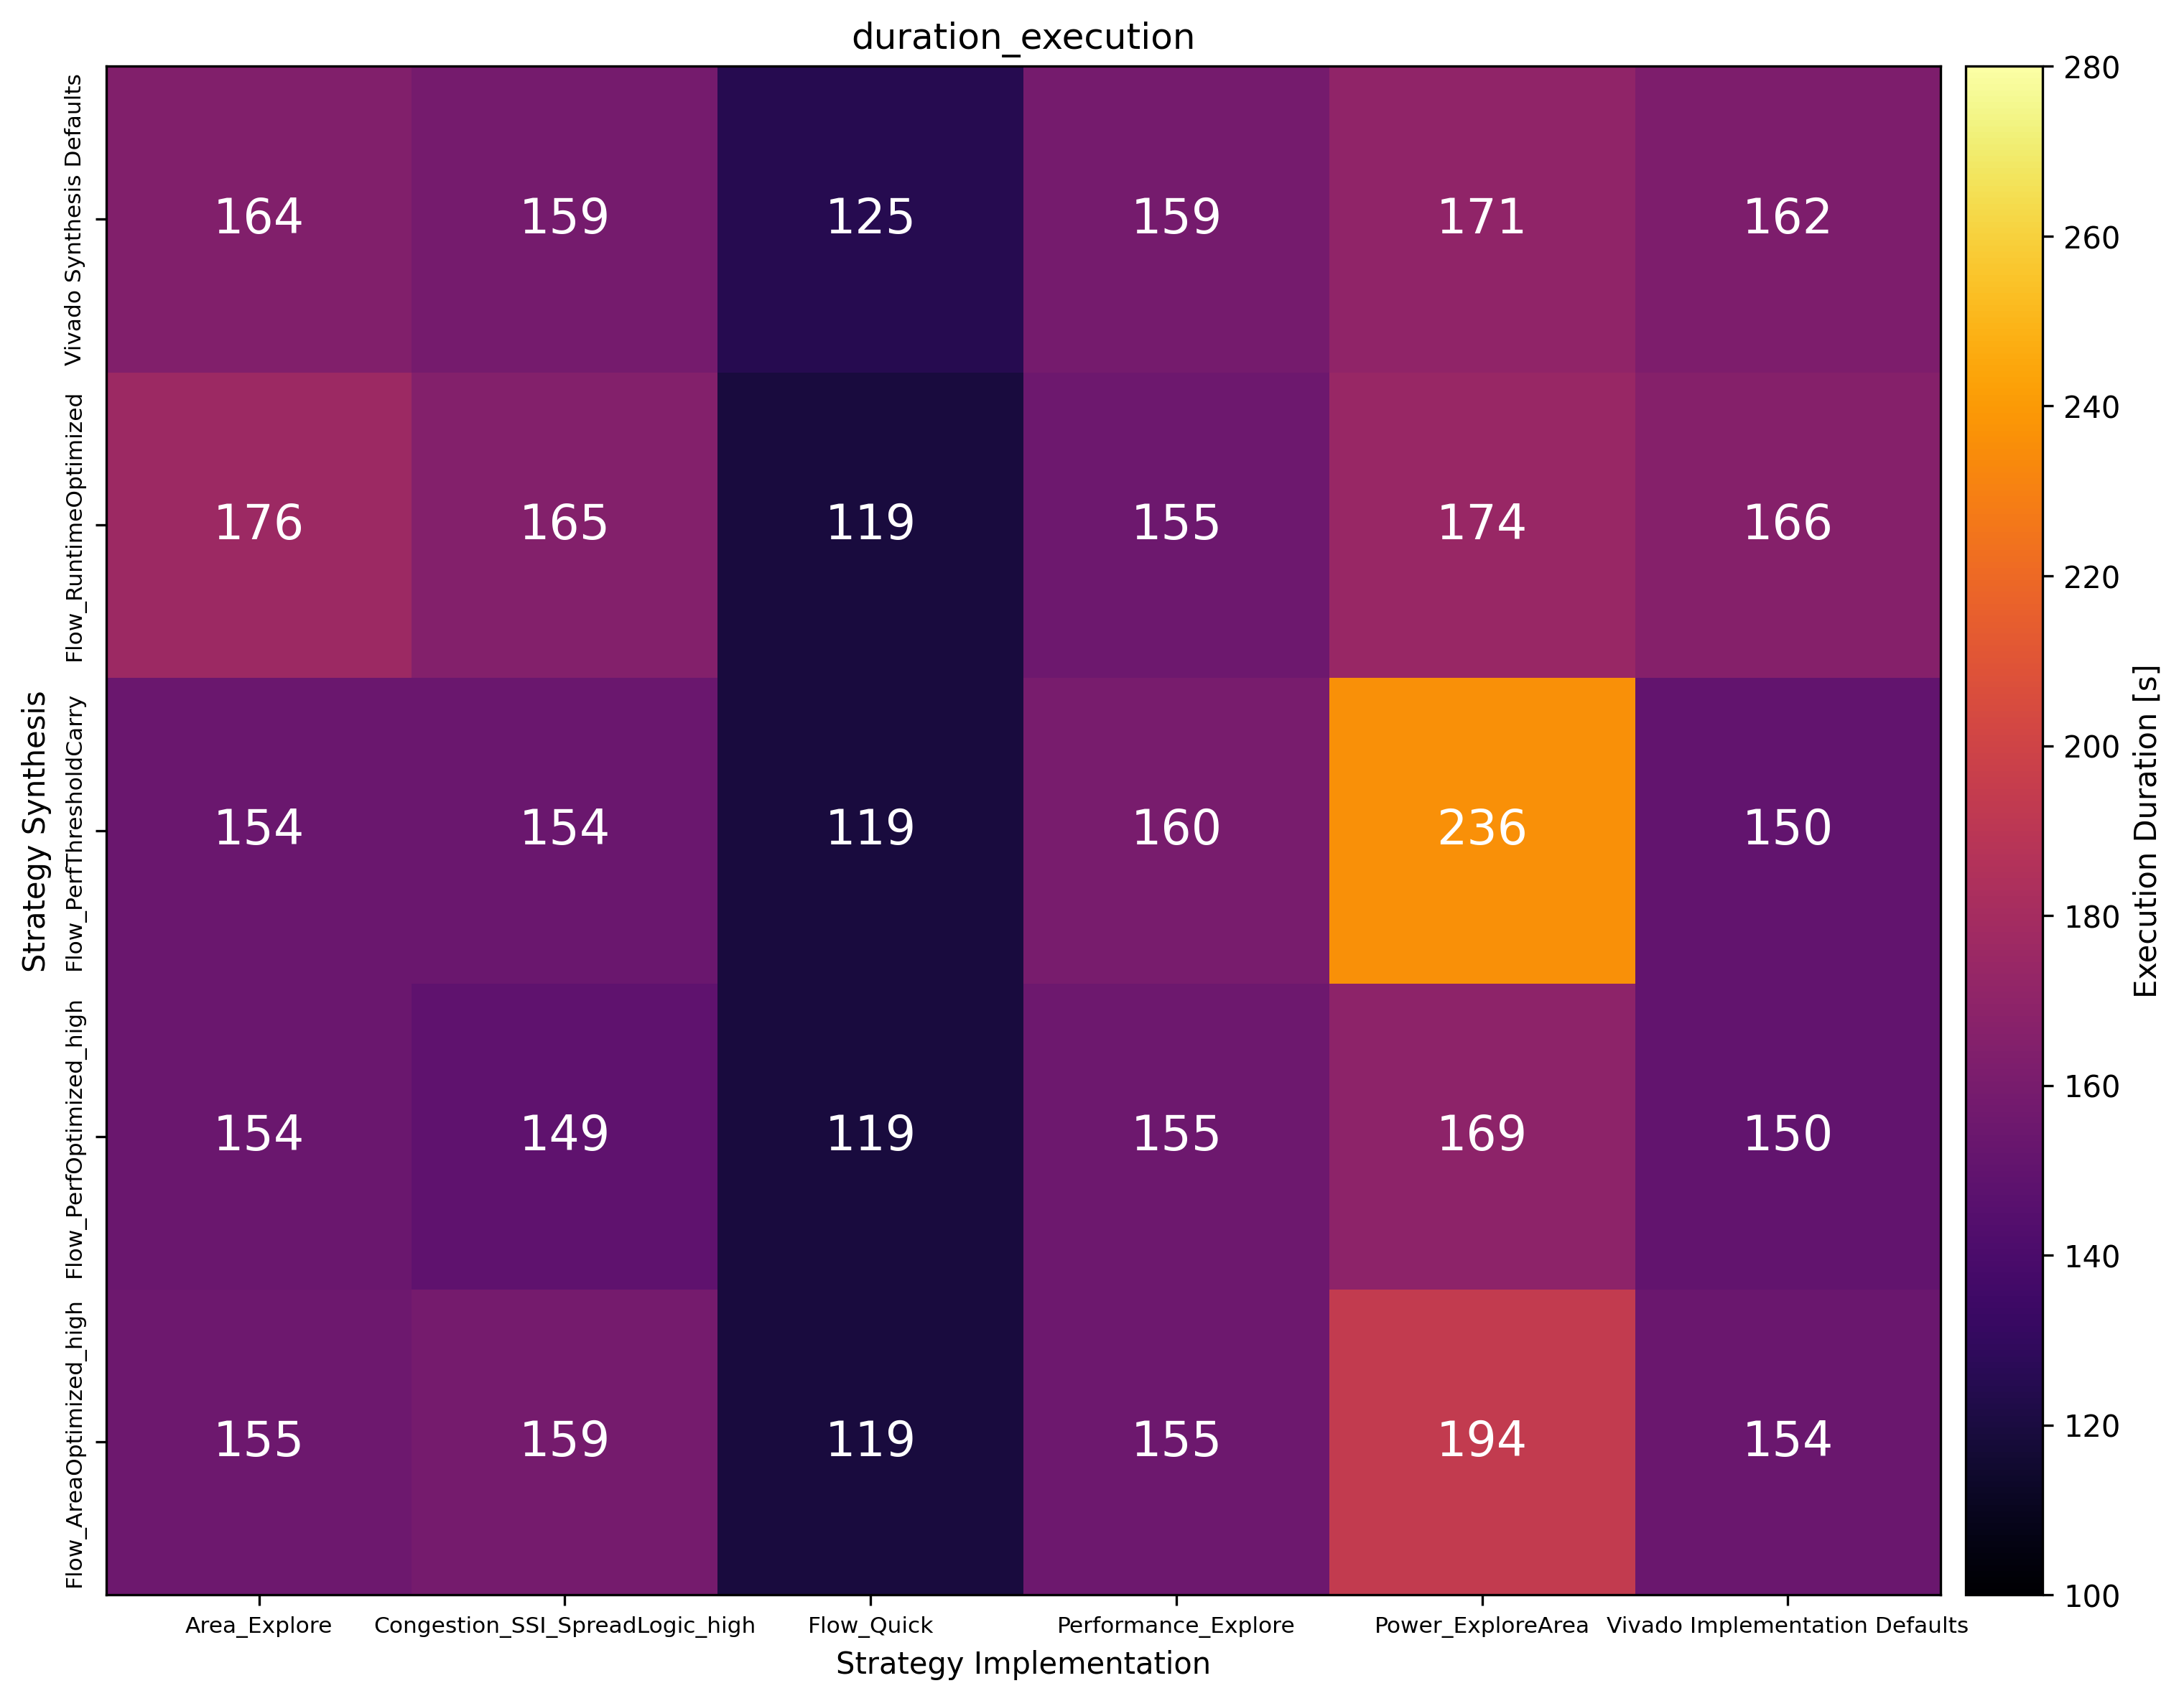
\includegraphics[width=\linewidth]{images/2_duration_execution.png}
        \caption{Duration Totale}
        \label{fig:duration_total_2}
    \end{subfigure}\hfill
	\begin{subfigure}[b]{0.30\textwidth}
        \centering
        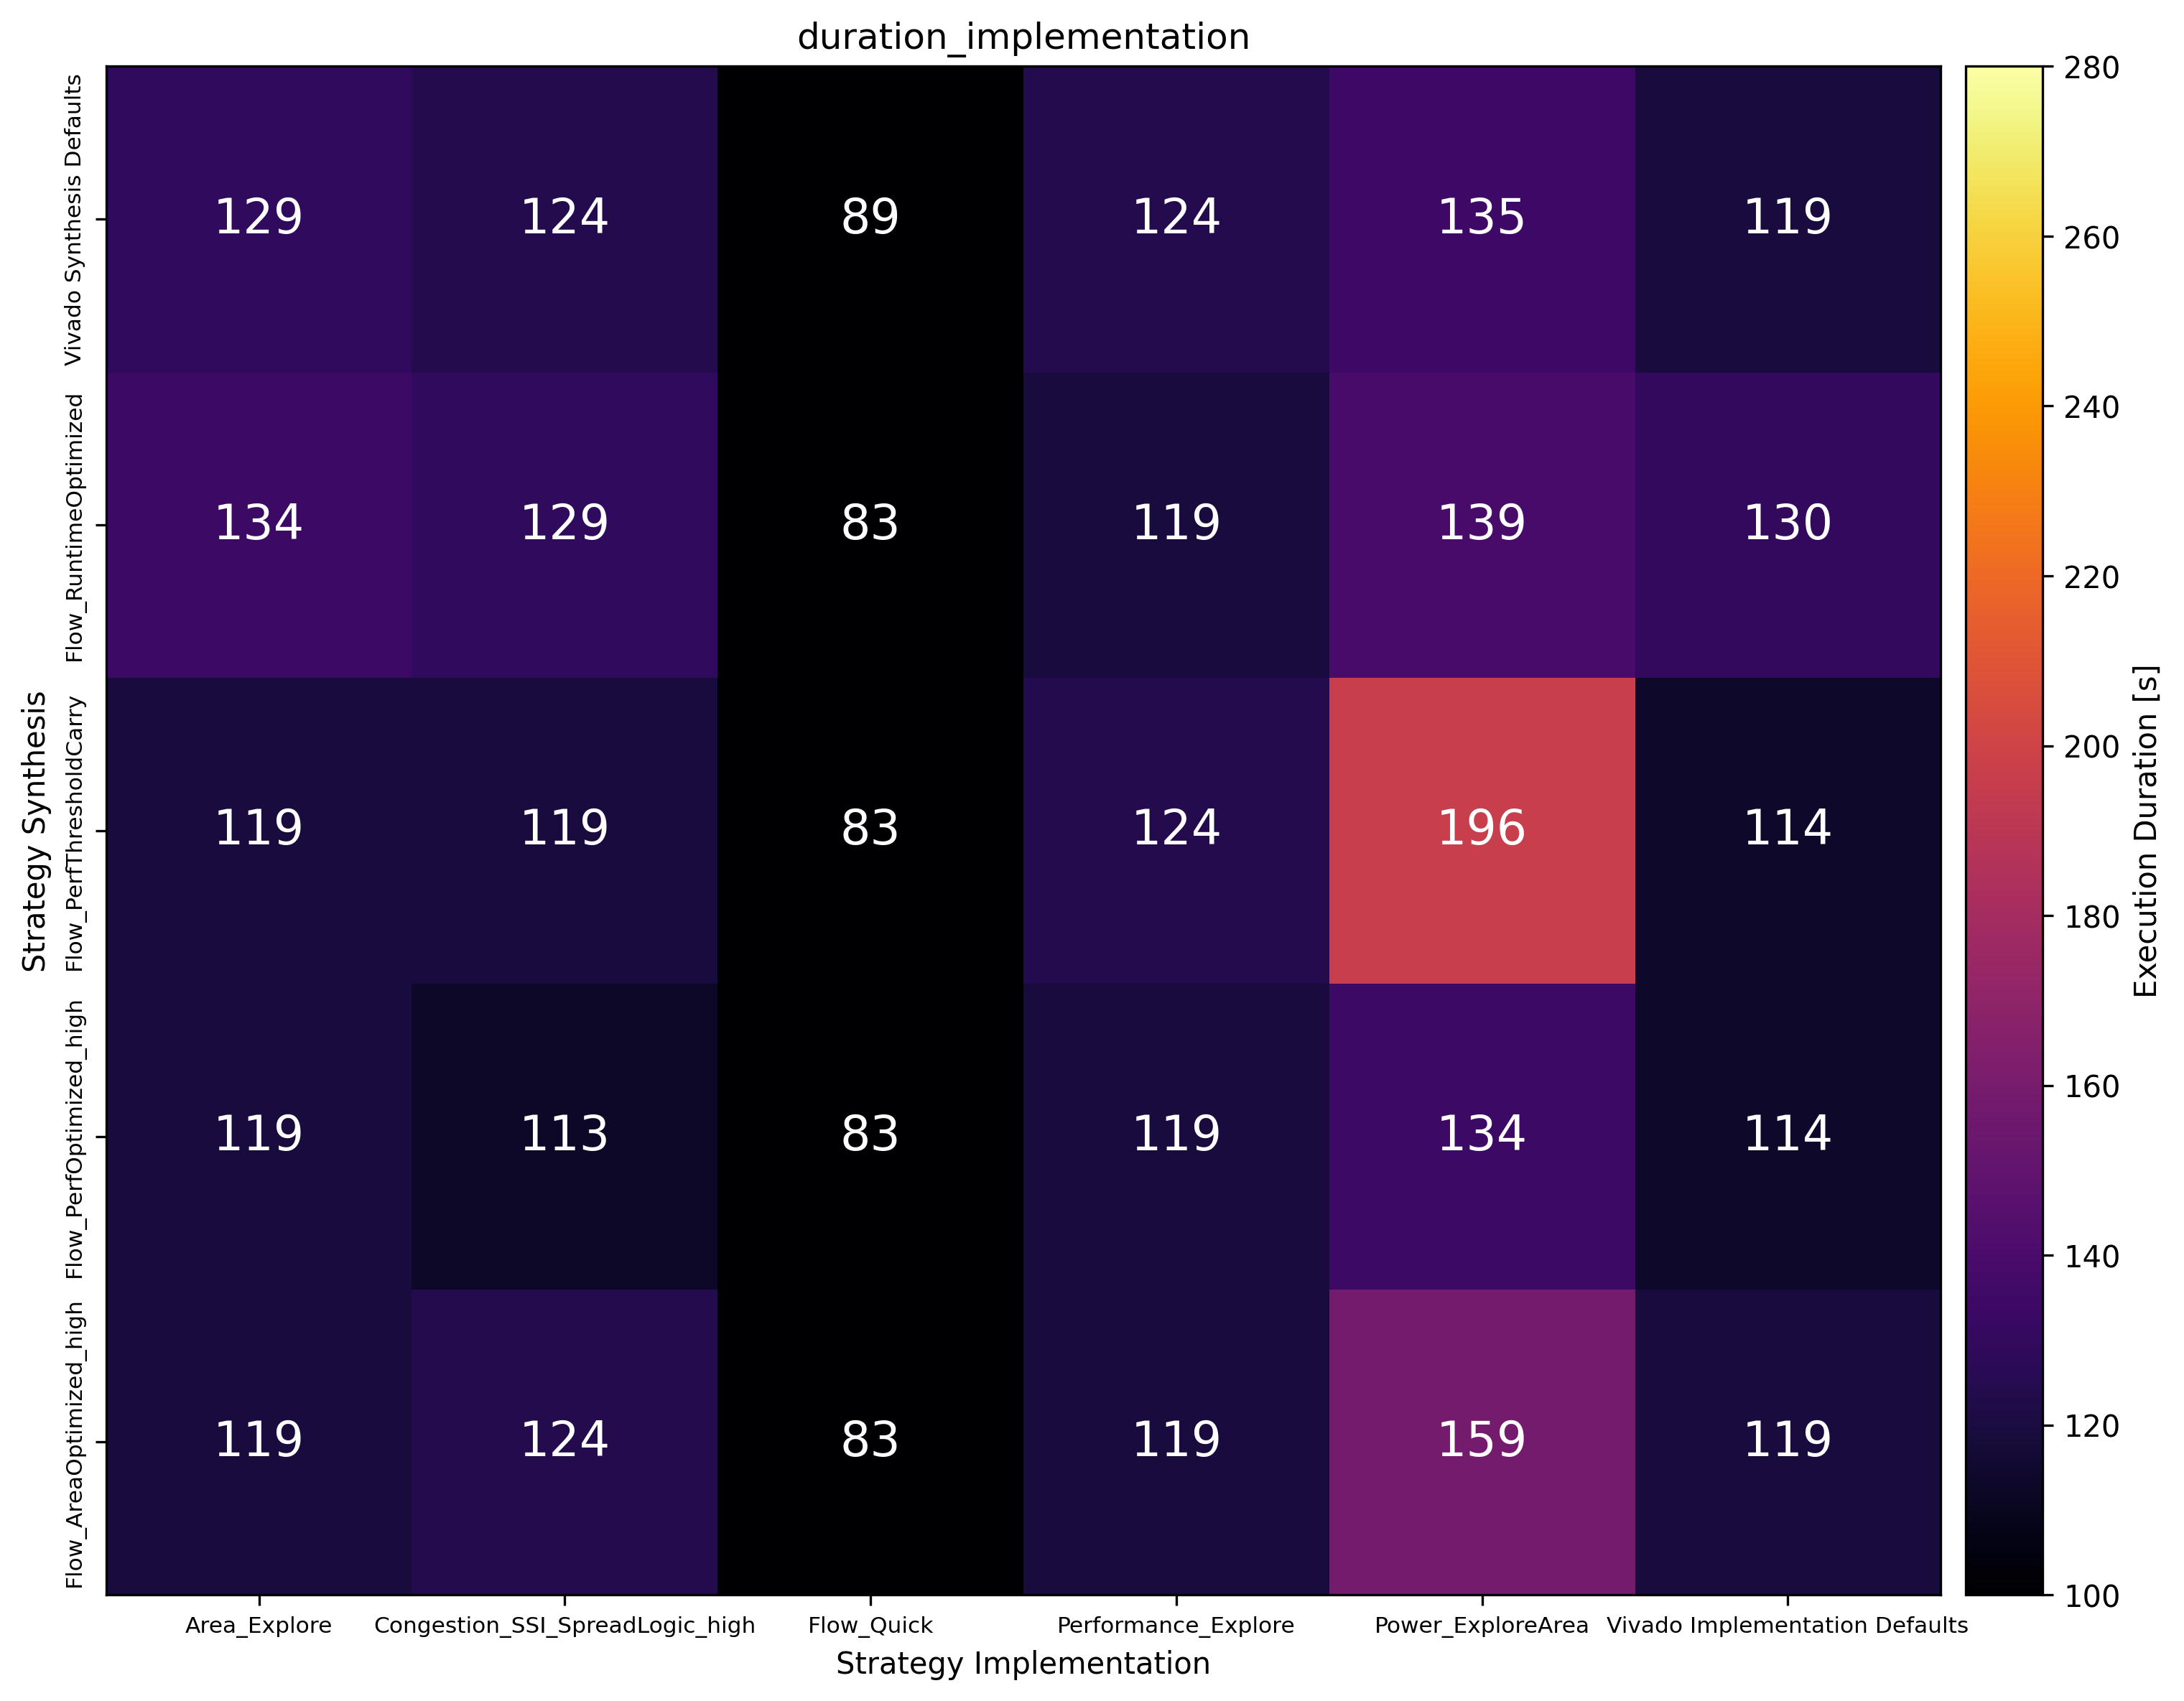
\includegraphics[width=\linewidth]{images/2_duration_implementation.png}
        \caption{Duration Implementation}
        \label{fig:duration_implementation_2}
    \end{subfigure}\hfill
    \begin{subfigure}[b]{0.30\textwidth}
        \centering
        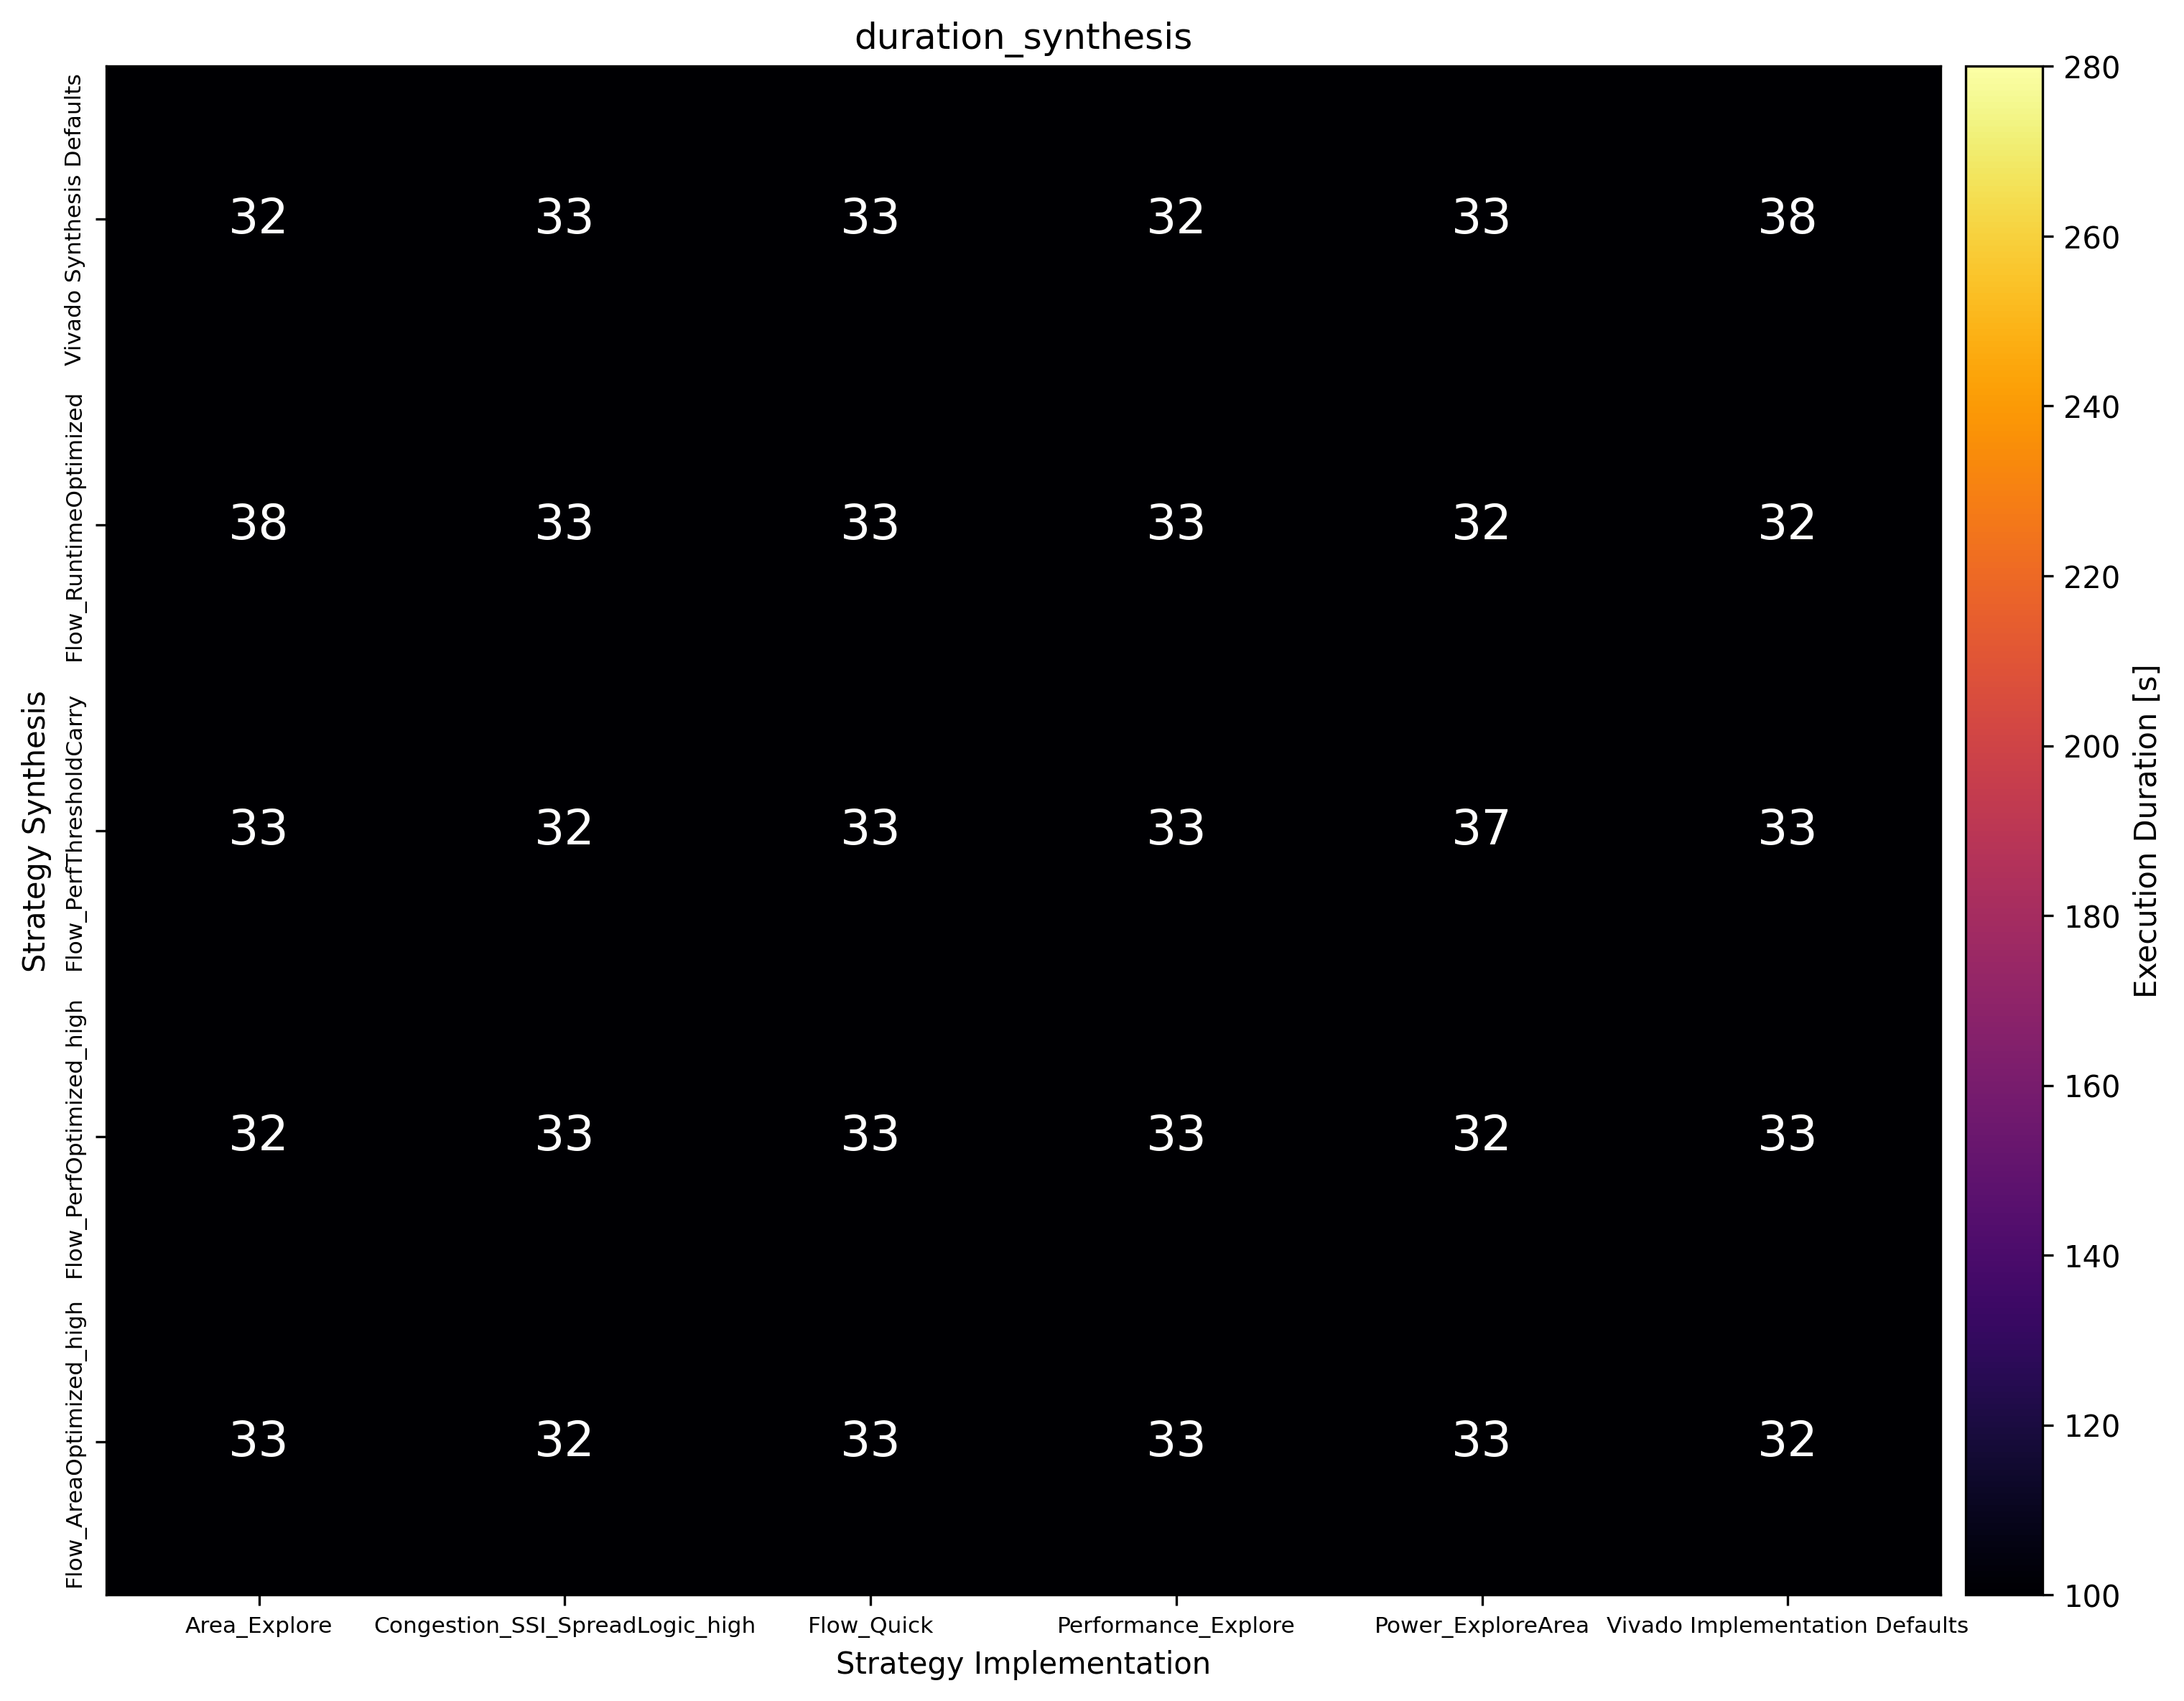
\includegraphics[width=\linewidth]{images/2_duration_synthesis.png}
        \caption{Duration Synthesis}
        \label{fig:duration_synthesis_2}
    \end{subfigure}
    \caption{Temps d'Éxécution de Simulation pour Synthèse et Implémentation}
    \label{fig:duration_2}
\end{figure}
\begin{remark}
    Il faut remarquer que le plus petit le valeur, le mieux.
\end{remark}
\begin{remark}
    Il faut remarquer que la Figure \ref{fig:duration_total_2} est égalé à la somme des Figures \ref{fig:duration_implementation_2} et \ref{fig:duration_synthesis_2}.
\end{remark}
\noindent Il est constaté qu'une stratégie d'implémentation présente systématiquement les temps d'exécution les plus courts, la "Flow\_Quick", qui, quel que soit le méthode de synthèse utilisée, affiche les temps les plus bas. Il est également à noter que la stratégie d'implémentation avec les temps d'exécution les plus élevés est la "Power\_ExploreArea", avec la méthode "Flow\_PathThresholdCarry" présentant une durée nettement plus longue que toutes les autres. Les autres combinaisons de méthodes ne montrent pas de résultats remarquables.\\

\noindent En analysant les graphiques indépendants des méthodes d'implémentation et de synthèse, on remarque que le principal facteur influençant le temps d'exécution est le temps d'implémentation, car les temps de synthèse sont essentiellement identiques pour toutes les combinaisons.


\subsubsection{Power}
\noindent Dans la séquence suivante, l'analyse porte sur les pertes de puissance simulées pour les circuits pour chaque combinaison de synthèse et d'implémentation, comme montré ci-dessous :
\begin{figure}[h]
    \centering
    \begin{subfigure}[b]{0.30\textwidth}
        \centering
        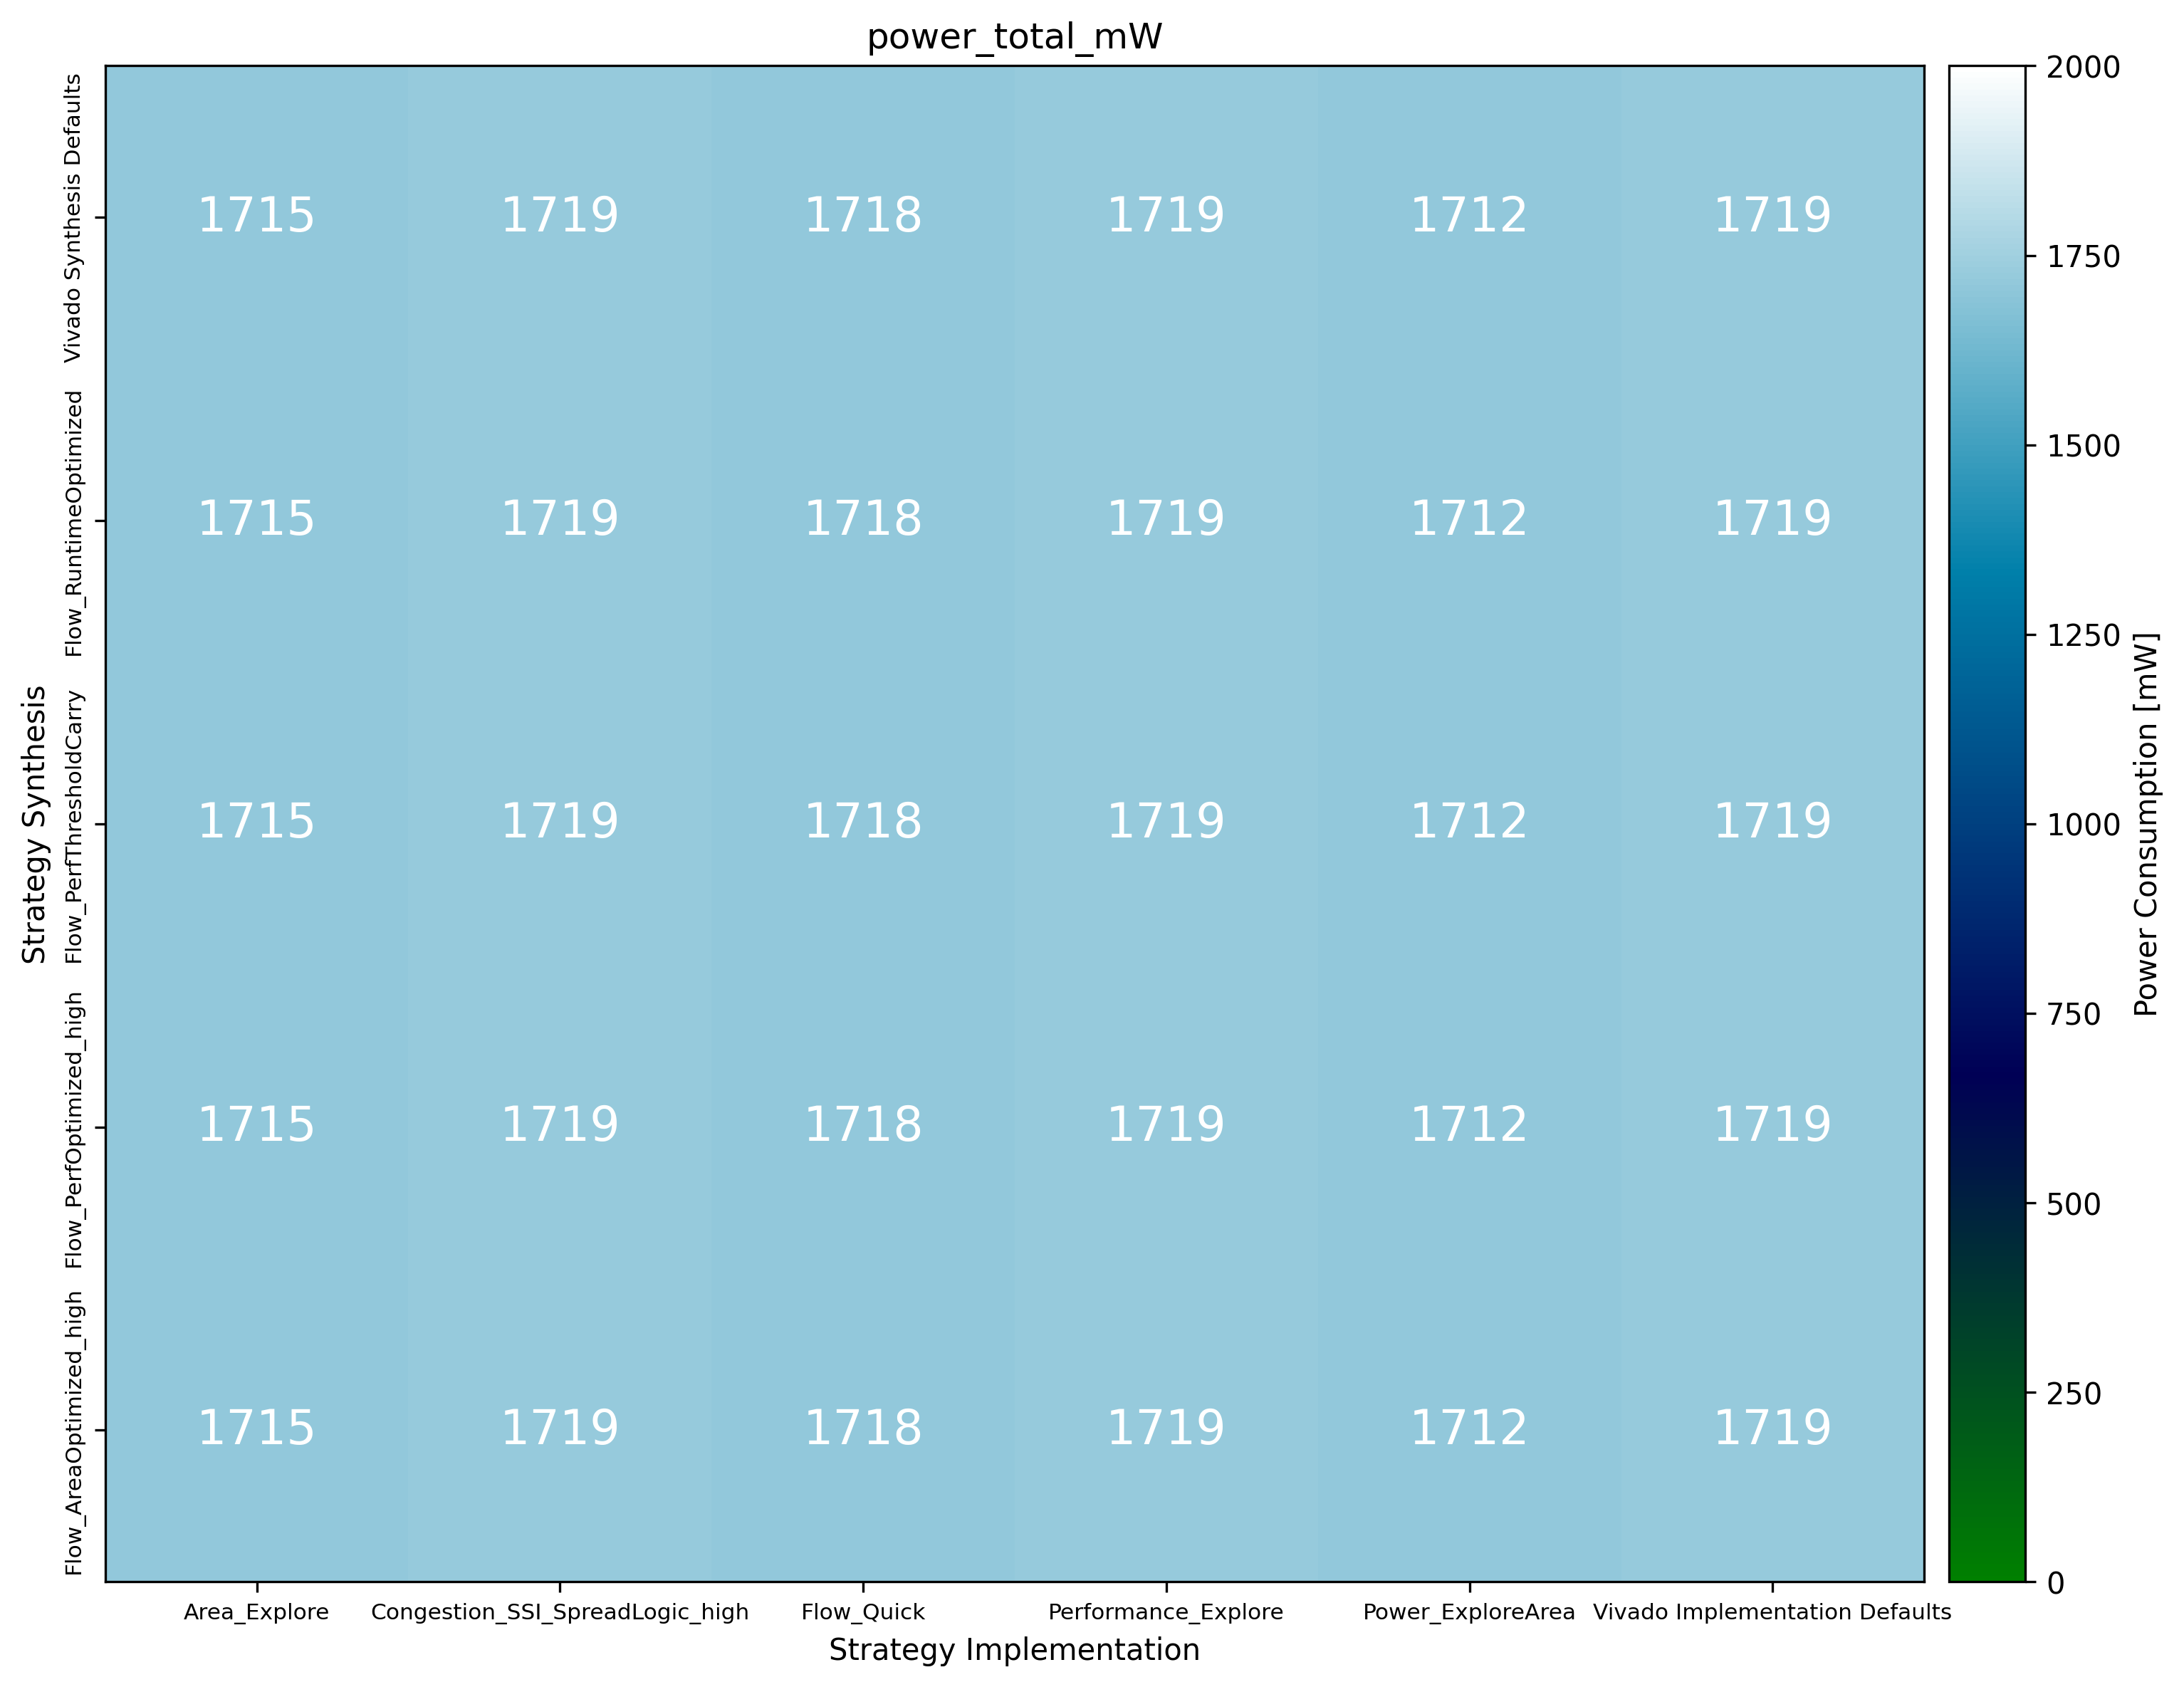
\includegraphics[width=\linewidth]{images/2_power_total_mW.png}
        \caption{Énergie Totale}
        \label{fig:power_total_2}
    \end{subfigure}\hfill
	\begin{subfigure}[b]{0.30\textwidth}
        \centering
        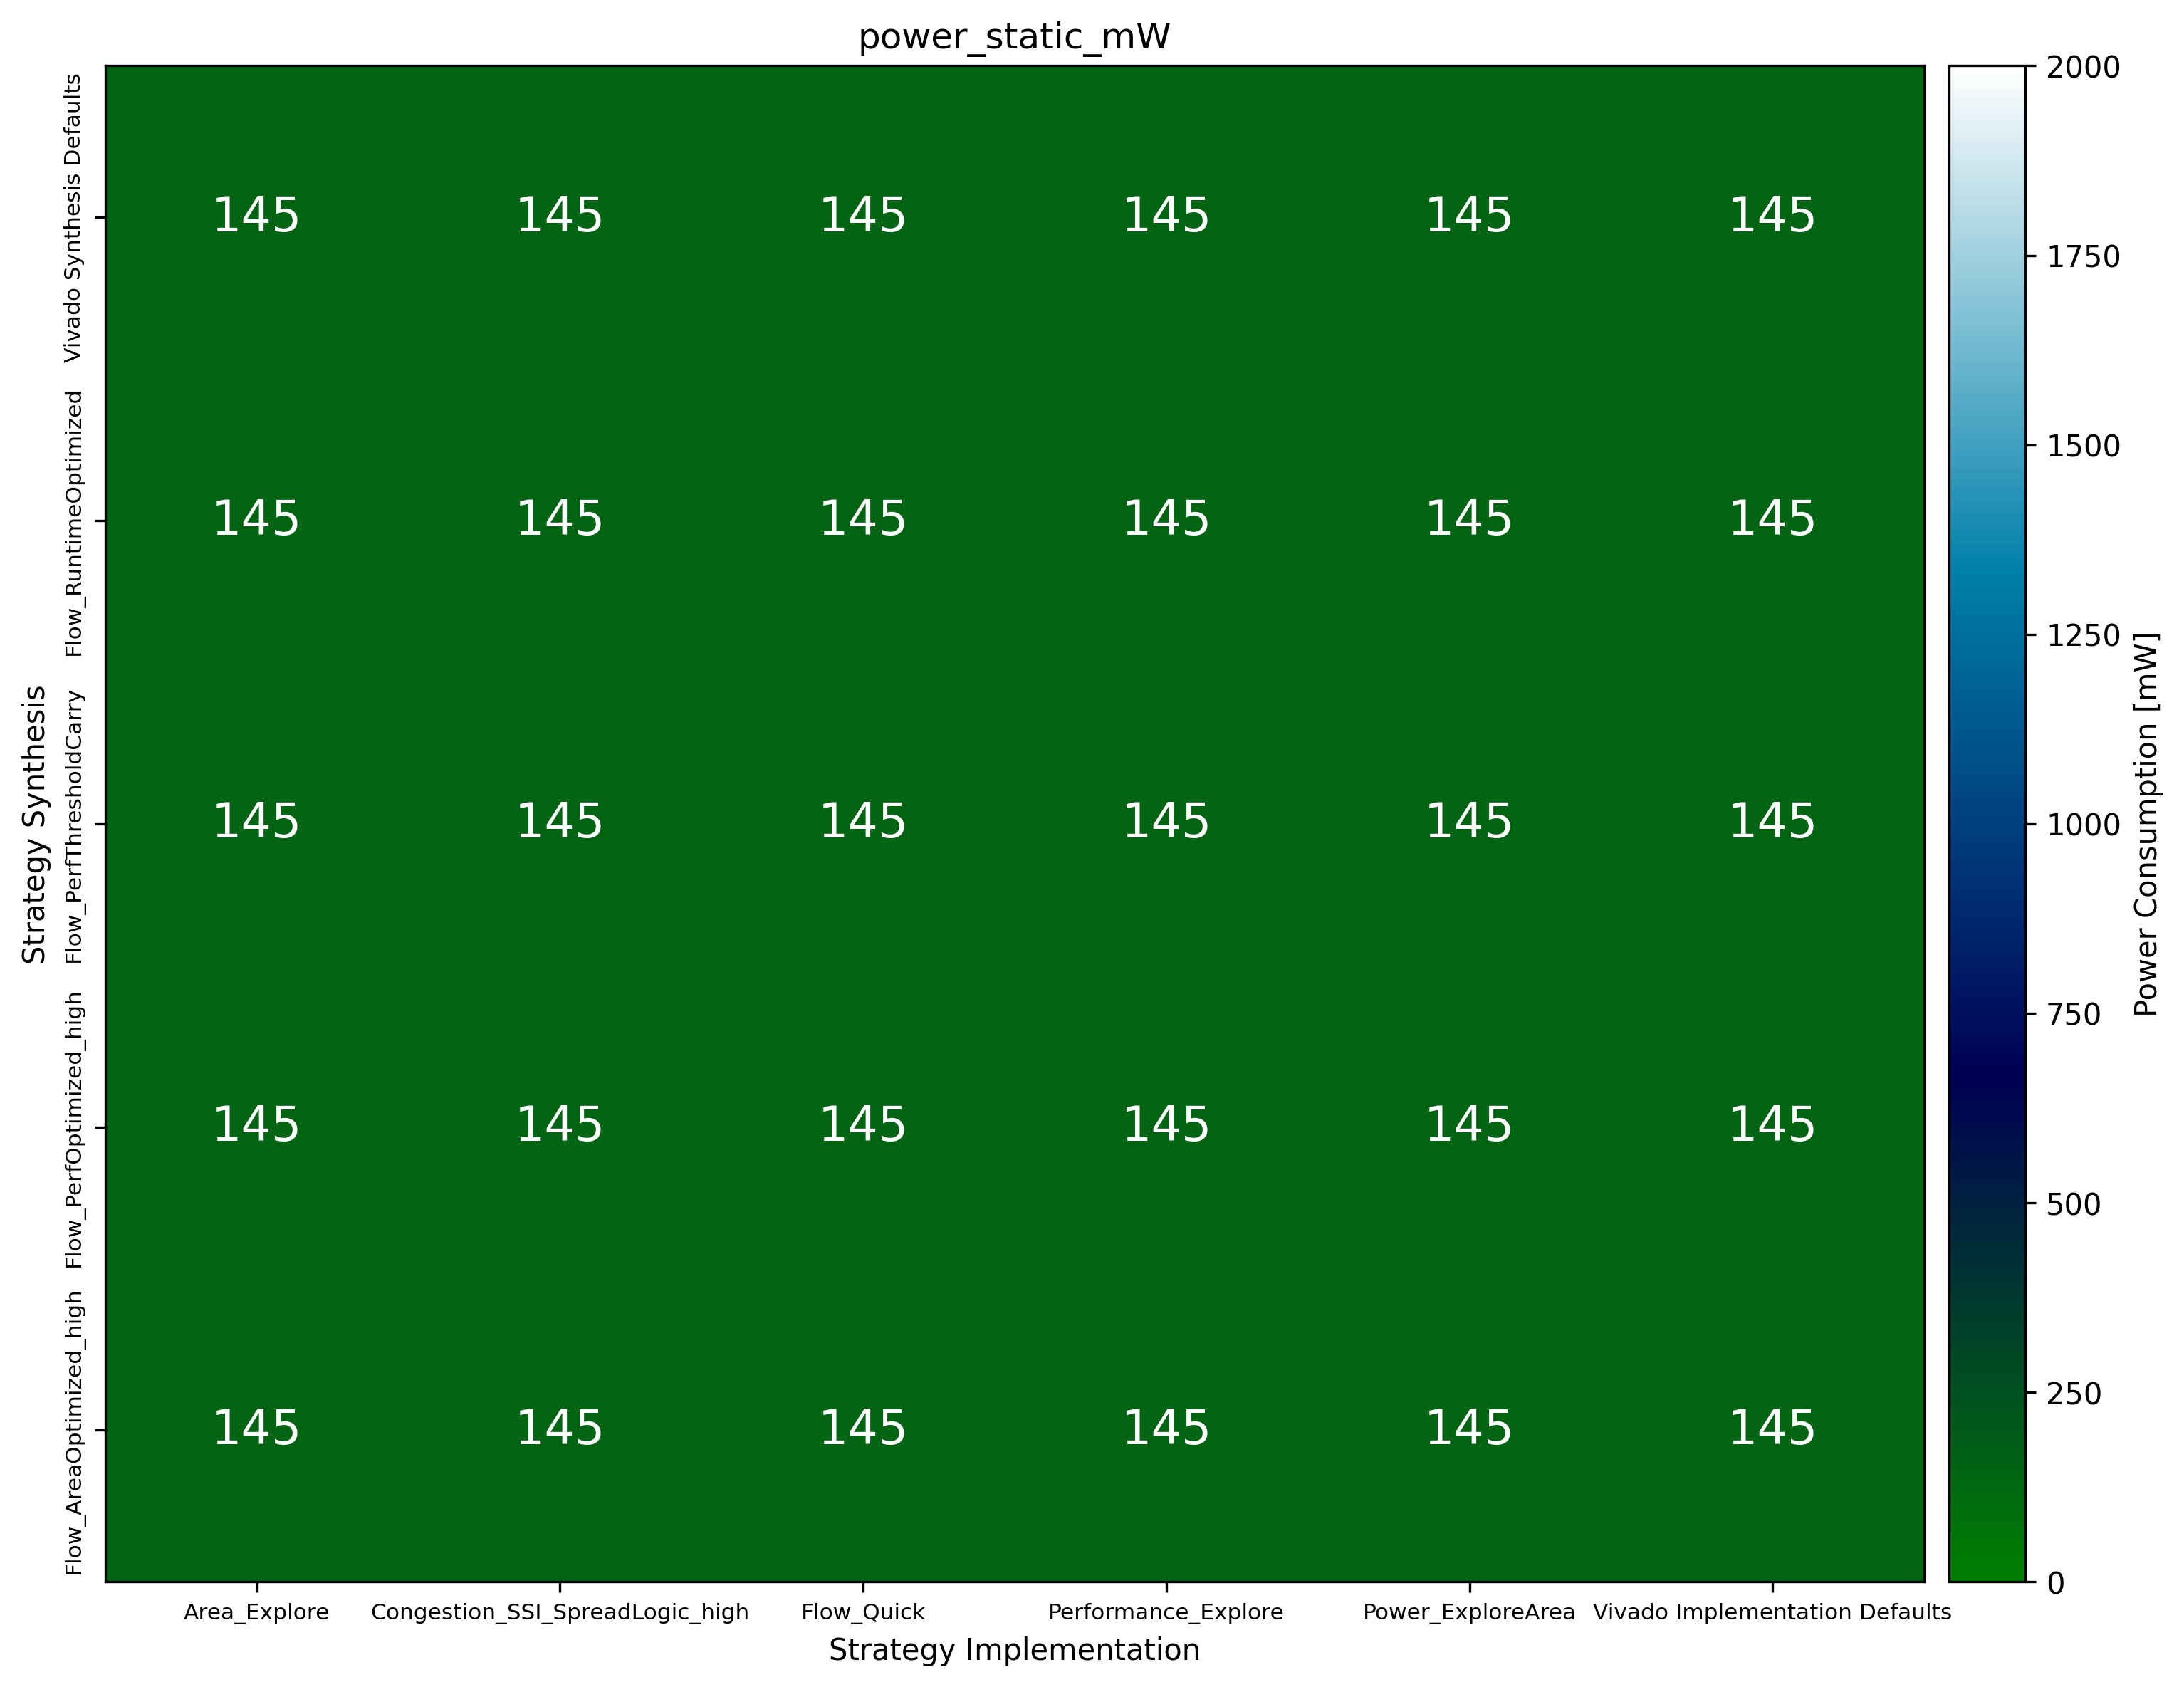
\includegraphics[width=\linewidth]{images/2_power_static_mW.png}
        \caption{Énergie Statique}
        \label{fig:power_static_2}
    \end{subfigure}\hfill
    \begin{subfigure}[b]{0.30\textwidth}
        \centering
        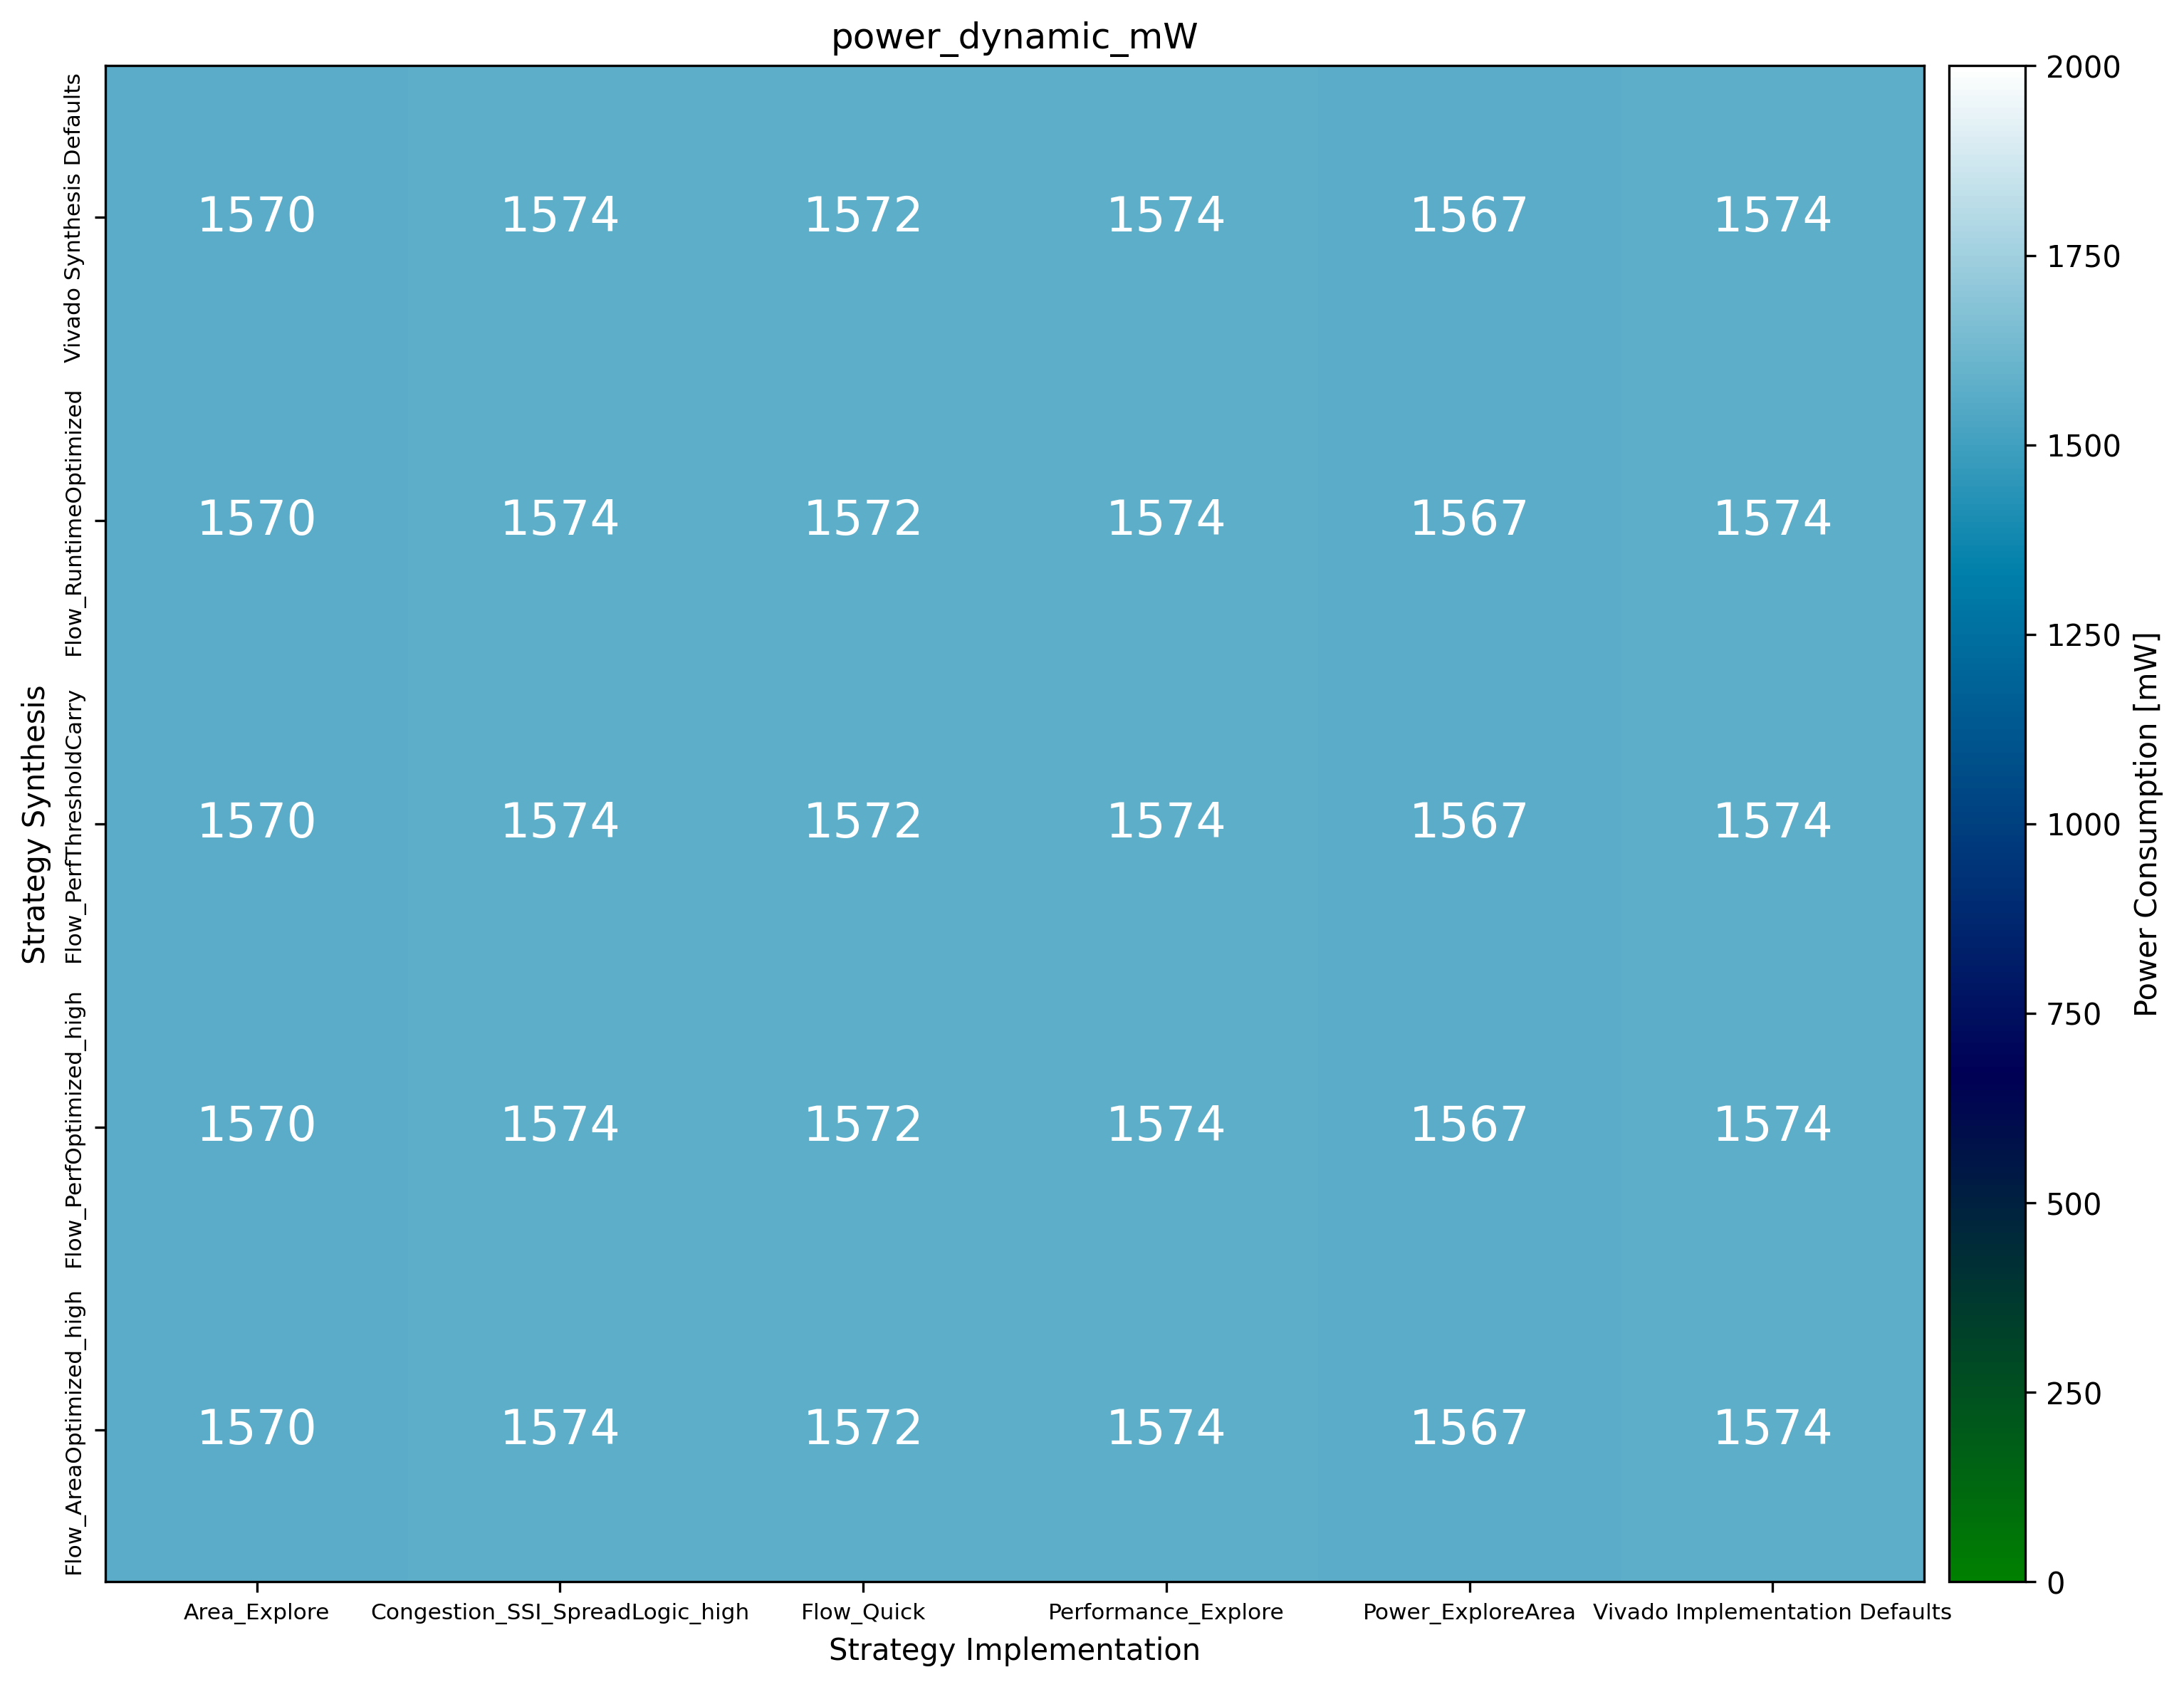
\includegraphics[width=\linewidth]{images/2_power_dynamic_mW.png}
        \caption{Énergie Dynamique}
        \label{fig:power_dynamic_2}
    \end{subfigure}
    \caption{Dissipacition d'Énergie de Simulation pour Synthèse et Implémentation}
    \label{fig:power_2}
\end{figure}
\begin{remark}
    Il faut remarquer que le plus petit le valeur, le mieux.
\end{remark}
\begin{remark}
    Il faut remarquer que la Figure \ref{fig:power_total_2} est égalé à la somme des Figures \ref{fig:power_static_2} et \ref{fig:power_dynamic_2}.
\end{remark}
\noindent Il est à noter que, globalement, les valeurs sont pratiquement identiques et qu'il n'y a pas de grande variabilité entre les différentes valeurs.\\

\noindent Ainsi, une analyse plus détaillée a été effectuée sur les configurations qui ont donné les meilleurs et les pires résultats en termes de temps d'exécution :
\begin{figure}[H]
    \centering
    \begin{subfigure}[b]{0.475\textwidth}
        \centering
        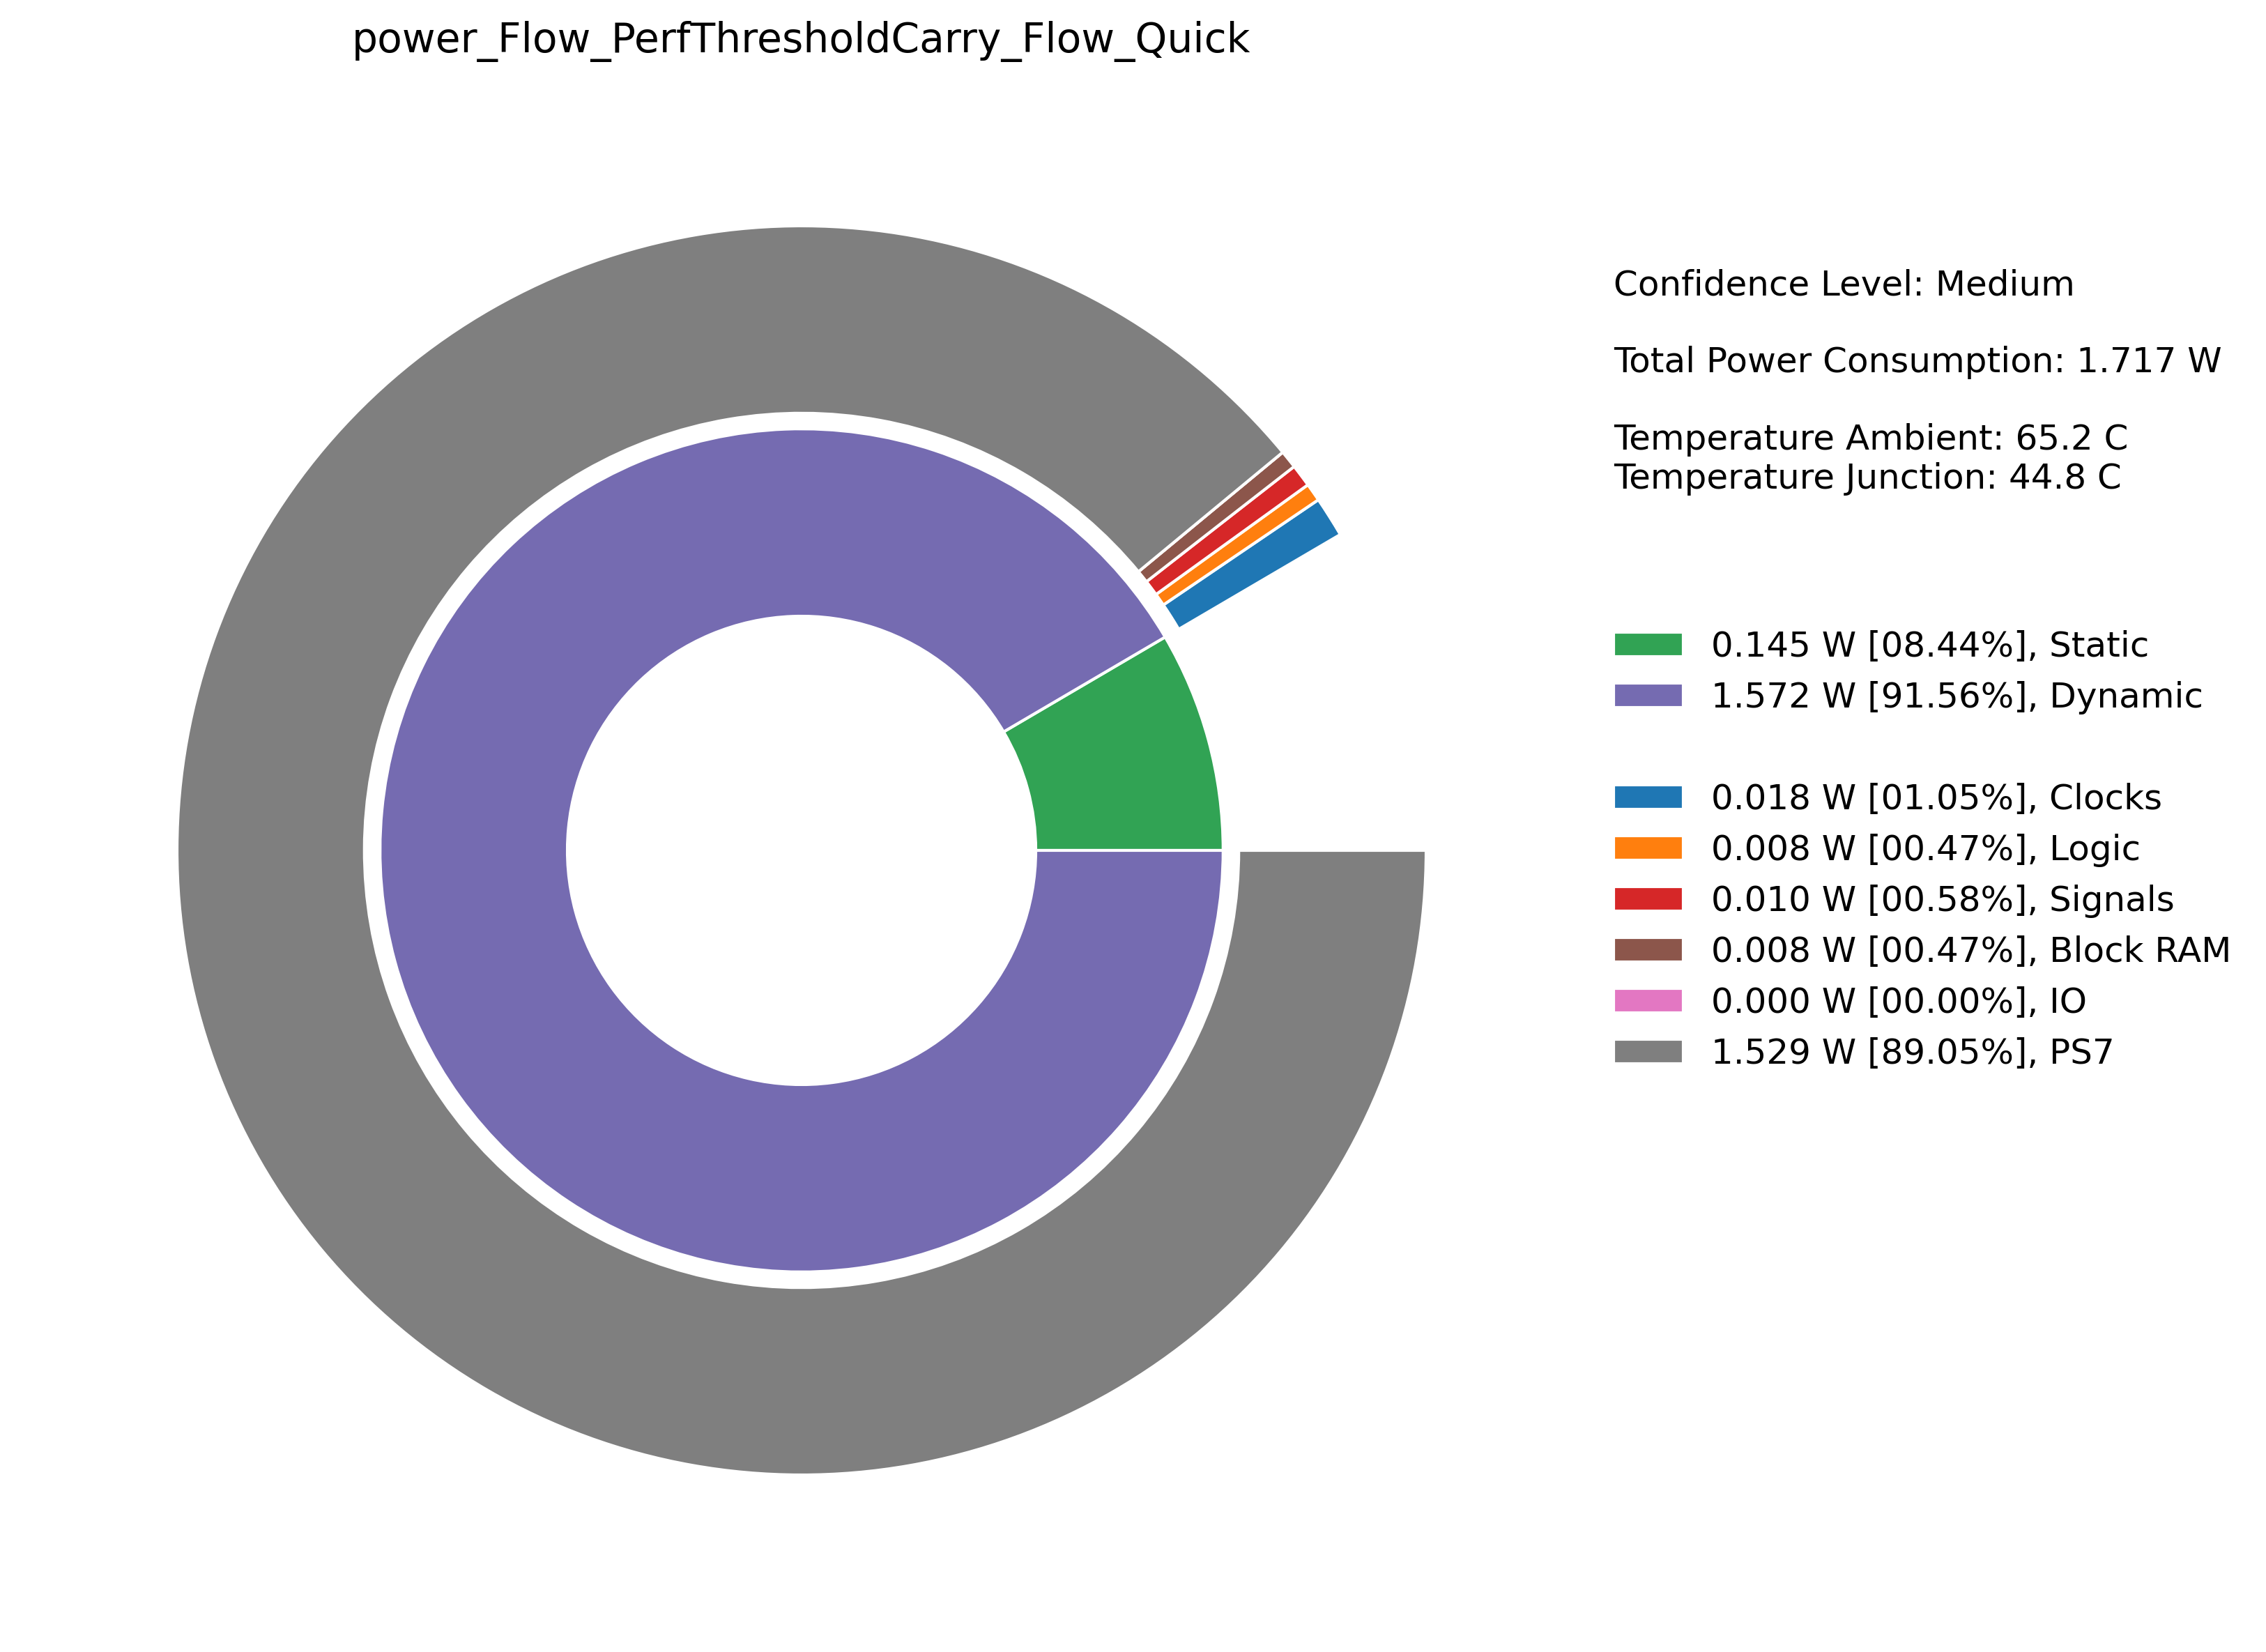
\includegraphics[width=\linewidth]{images/2_power_Flow_PerfThresholdCarry_Flow_Quick.png}
        \caption{\texttt{Flow\_PerfThresholdCarry} et \texttt{Flow\_Quick}}
    \end{subfigure}\hfill
    \begin{subfigure}[b]{0.475\textwidth}
        \centering
        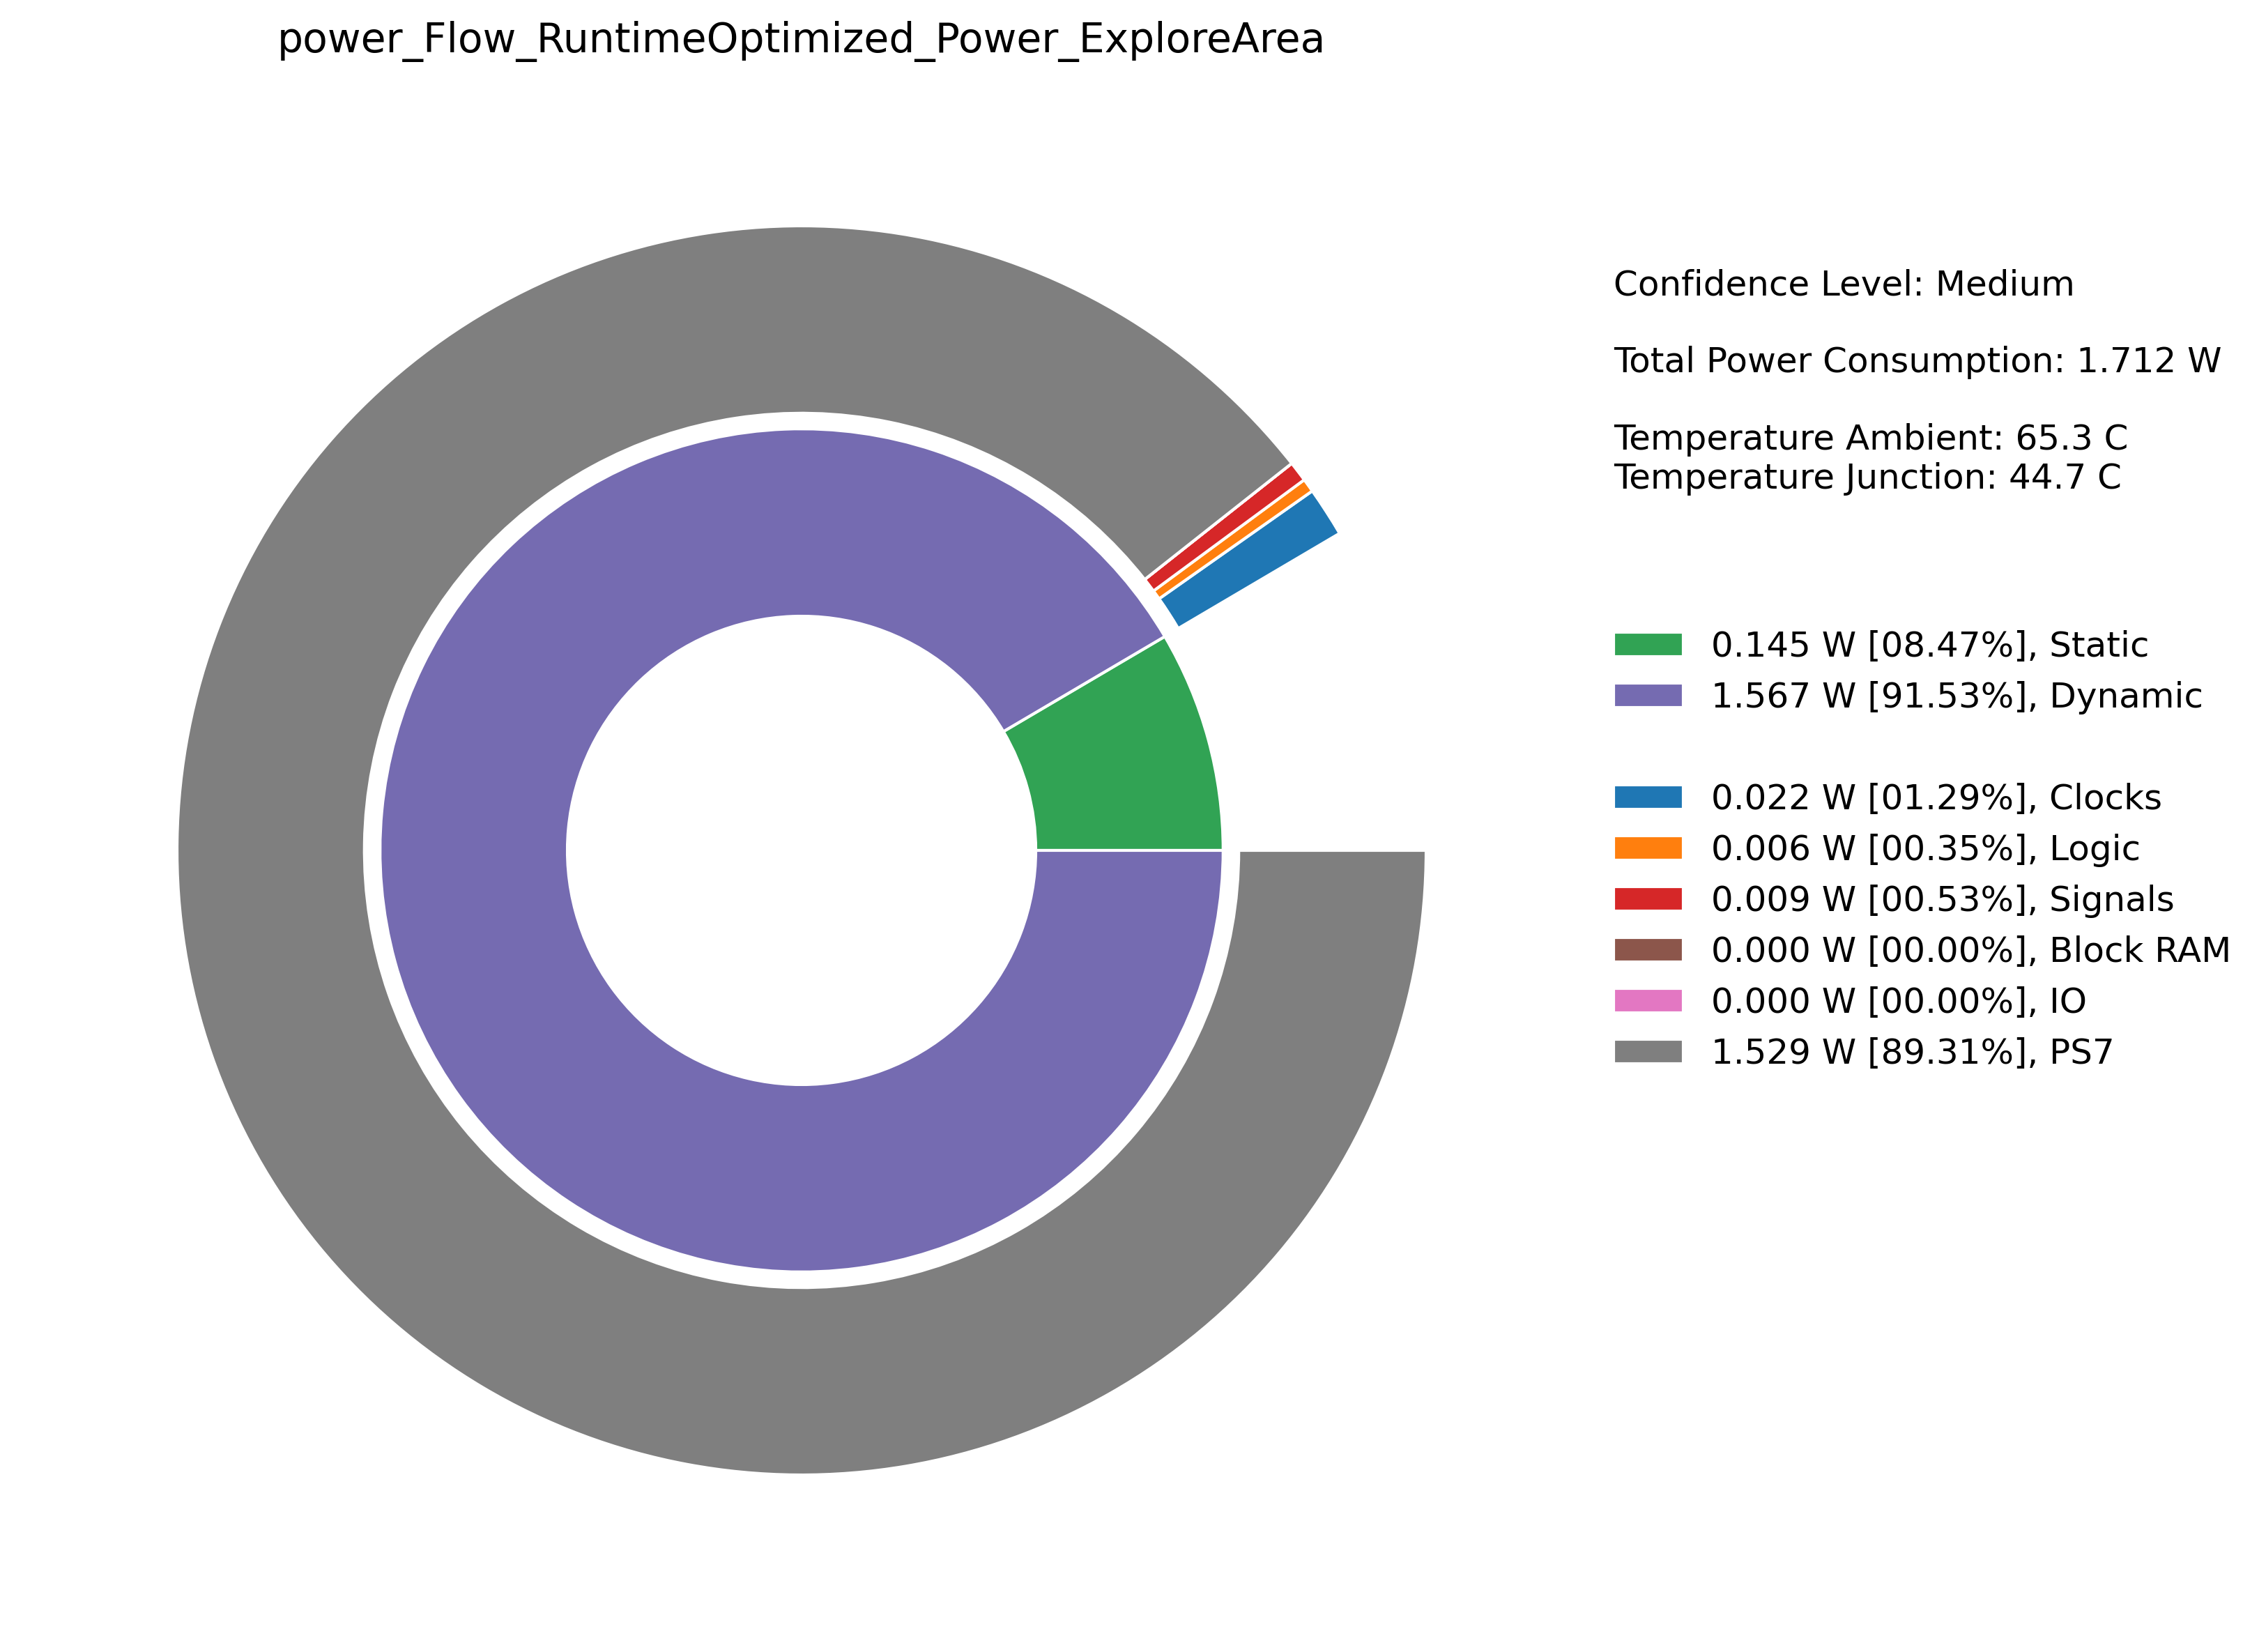
\includegraphics[width=\linewidth]{images/2_power_Flow_RuntimeOptimized_Power_ExploreArea.png}
        \caption{\texttt{Flow\_RuntimeOptimized} et \texttt{Power\_ExploreArea}}
    \end{subfigure}
    \caption{Détail de Dissicipation d'Énergie}
    \label{fig:power_detail_2}
\end{figure}
\noindent Il n'y a pas de grande variabilité entre les différentes combinaisons et, de ce fait, on conclut que la puissance dissipée est peu influencée par les méthodes d'implémentation ou de synthèse utilisées.

\subsubsection{WNS}
\noindent On passe maintenant à l'analyse du "Worst Negative Slack (WNS)" pour les différentes combinaisons de synthèse et d'implémentation, comme démontré ci-dessous :
\begin{figure}[H]
	\centering
	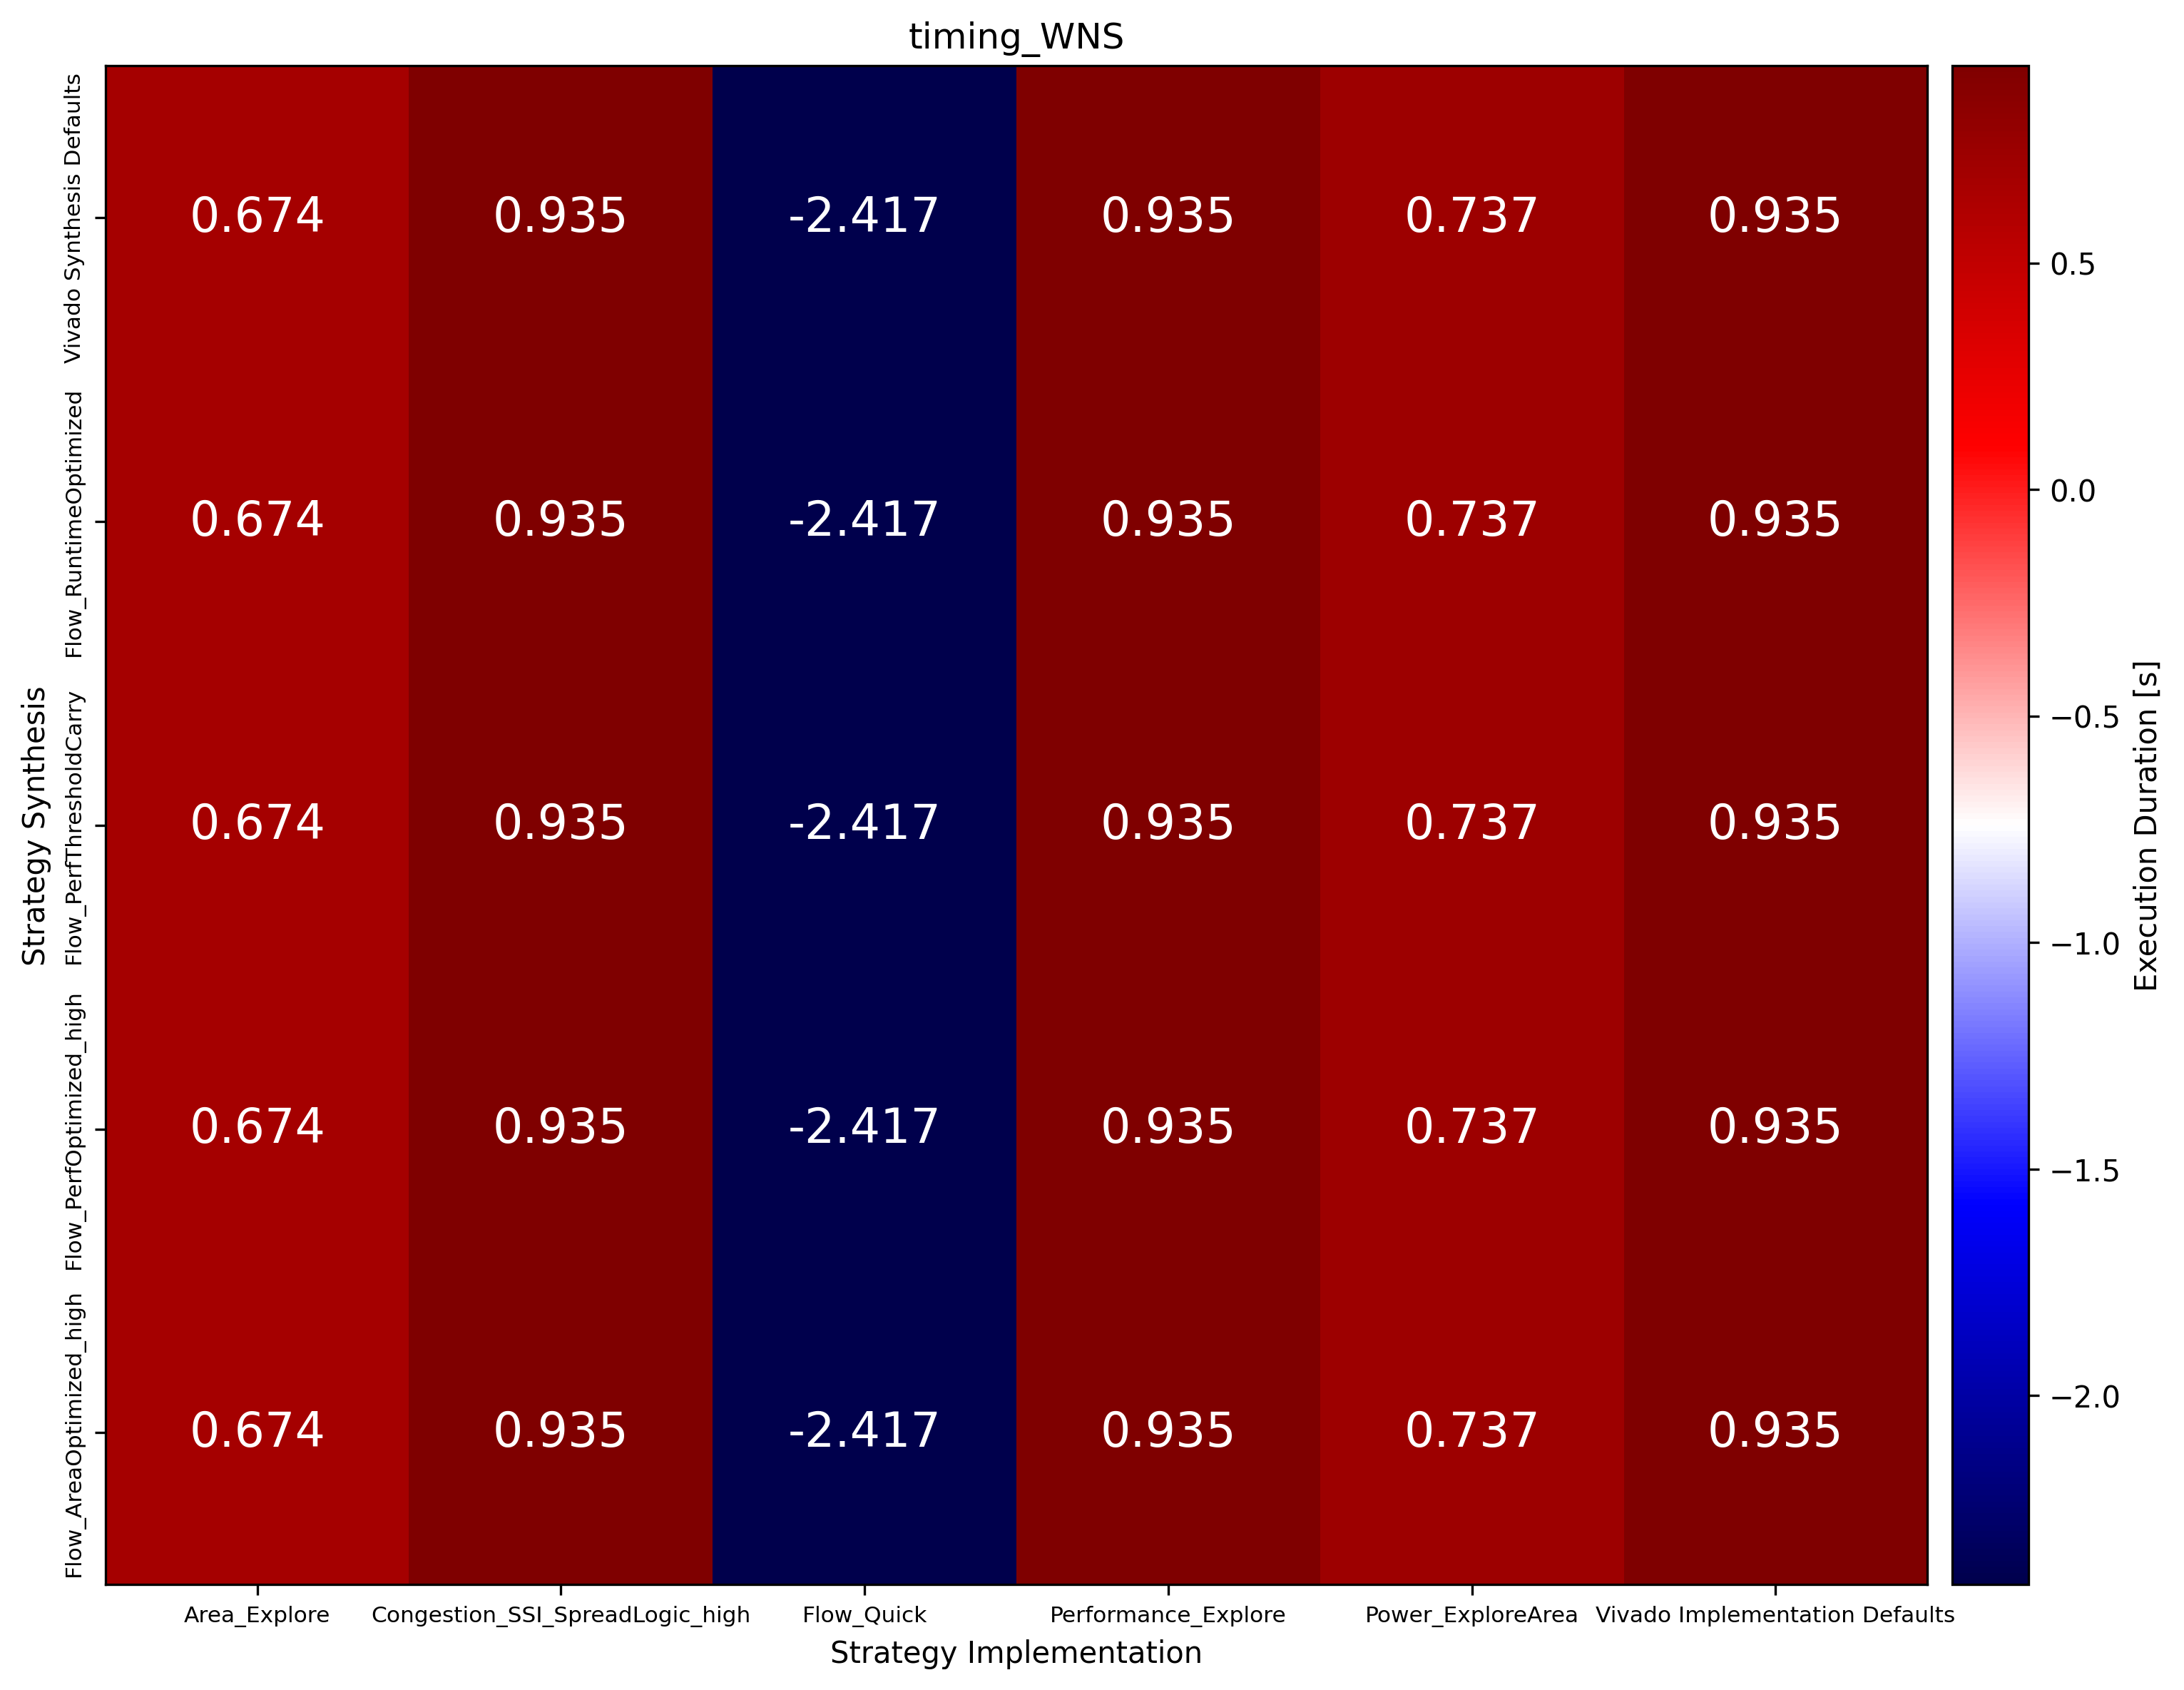
\includegraphics[width=0.5\linewidth]{images/2_timing_WNS.png}
	\caption{WNS Timing pour Synthèse et Implémentation}
	\label{fig:wns_2}
\end{figure}
\begin{remark}
    Il faut remarquer que le plus proche de zéro, le mieux. En cas négatif, sous-optimale.
\end{remark}
\noindent Ici, il devient évident que le compromis est fait entre le temps d'exécution et le WNS. La combinaison de "Flow\_PerfThresholdCarry" et "Power\_ExploreArea" présente la deuxième meilleure performance de WNS, tandis que la combinaison de "Flow\_RuntimeOptimized" et "Flow\_Quick" présente la pire performance de WNS, ce qui démontre que l'exécution a été plus courte car une solution n'a pas été trouvée.\\

\noindent Il est important de souligner que le choix de la stratégie de synthèse n'a pas influencé le résultat du WNS, étant donné que la stratégie d'implémentation est le principal facteur déterminant du résultat.


\subsubsection{Ressources}
\noindent Enfin, l'analyse de l'utilisation des ressources pour les différentes combinaisons de synthèse et d'implémentation est effectuée comme démontré ci-dessous :
\begin{figure}[H]
	\centering
	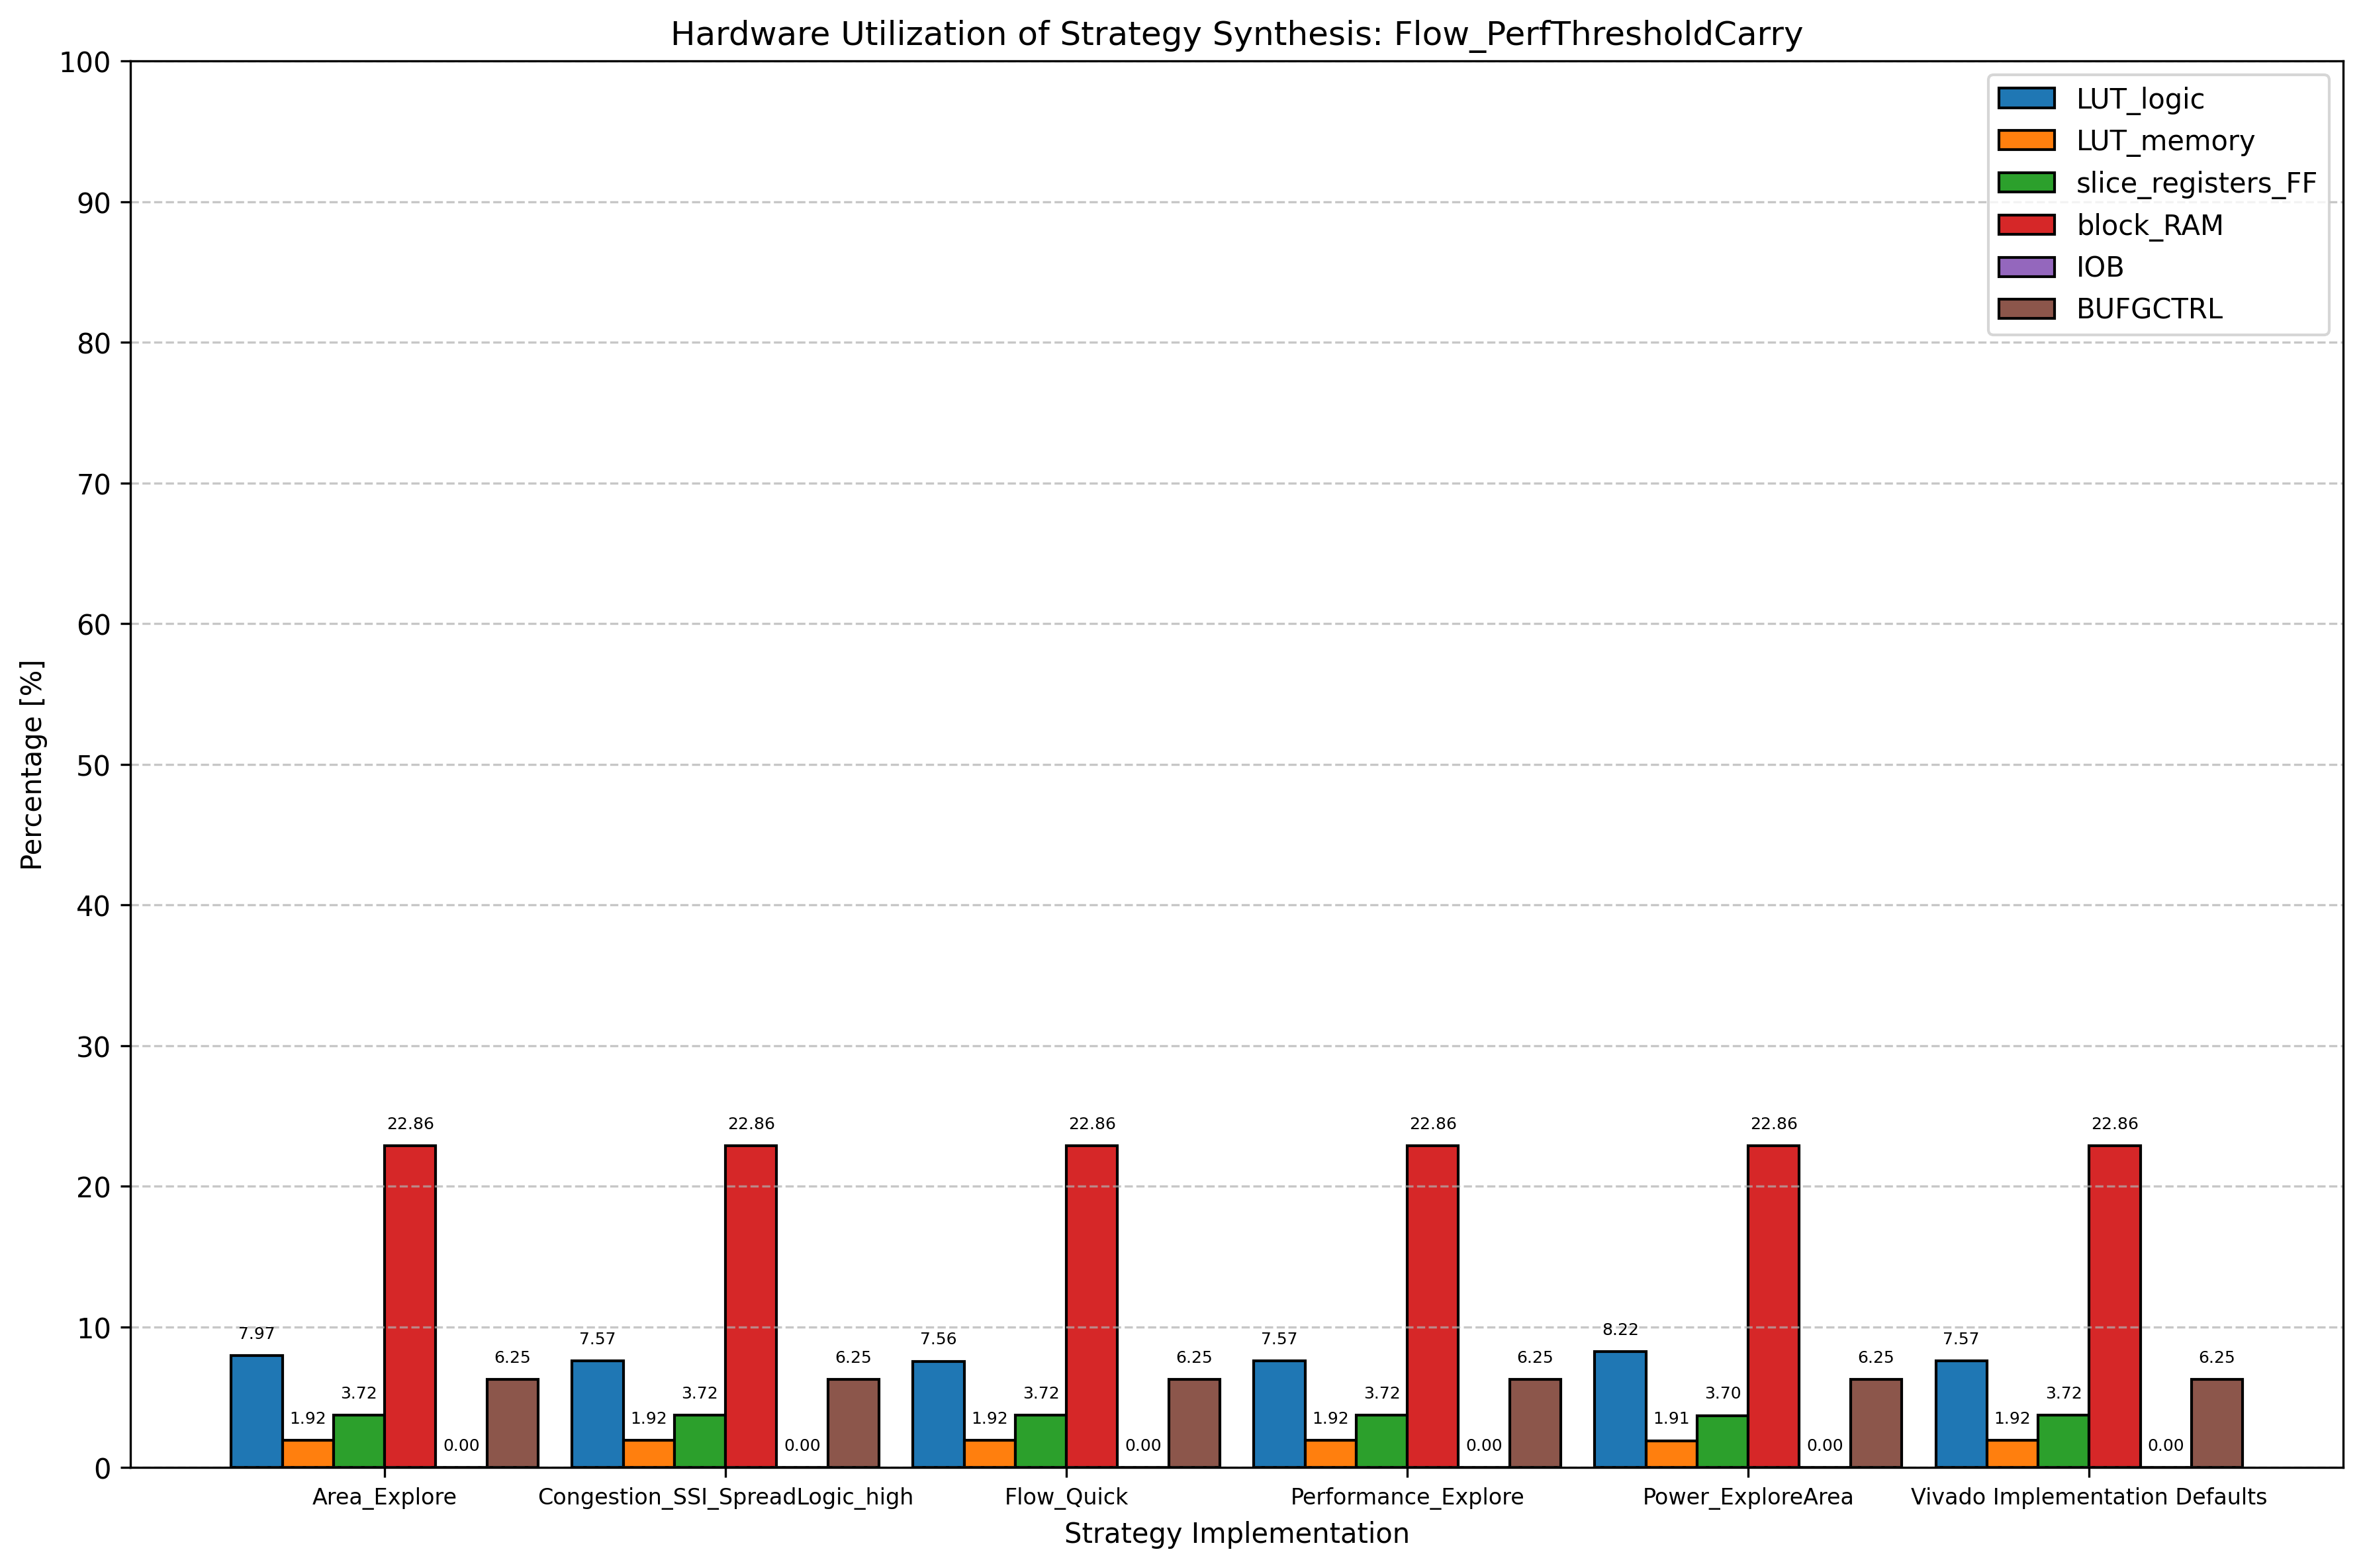
\includegraphics[width=0.5\linewidth]{images/2_utilization_Flow_PerfThresholdCarry.png}
	\caption{Utilization de Ressources pour \texttt{Flow\_PerfThresholdCarry}}
	\label{fig:ressouces_2}
\end{figure}
\begin{remark}
    Il faut remarquer que le plus petit, le mieux.
\end{remark}
\noindent Il n'y a pas de variations significatives dans l'utilisation des ressources matérielles entre les différentes configurations d'implémentation.



\subsection{Résultats Q3}
\subsubsection{Duration}
\noindent L'analyse commence par les temps d'exécution pour chaque combinaison de synthèse et d'implémentation, comme indiqué ci-dessous :
\begin{figure}[h]
    \centering
    \begin{subfigure}[b]{0.30\textwidth}
        \centering
        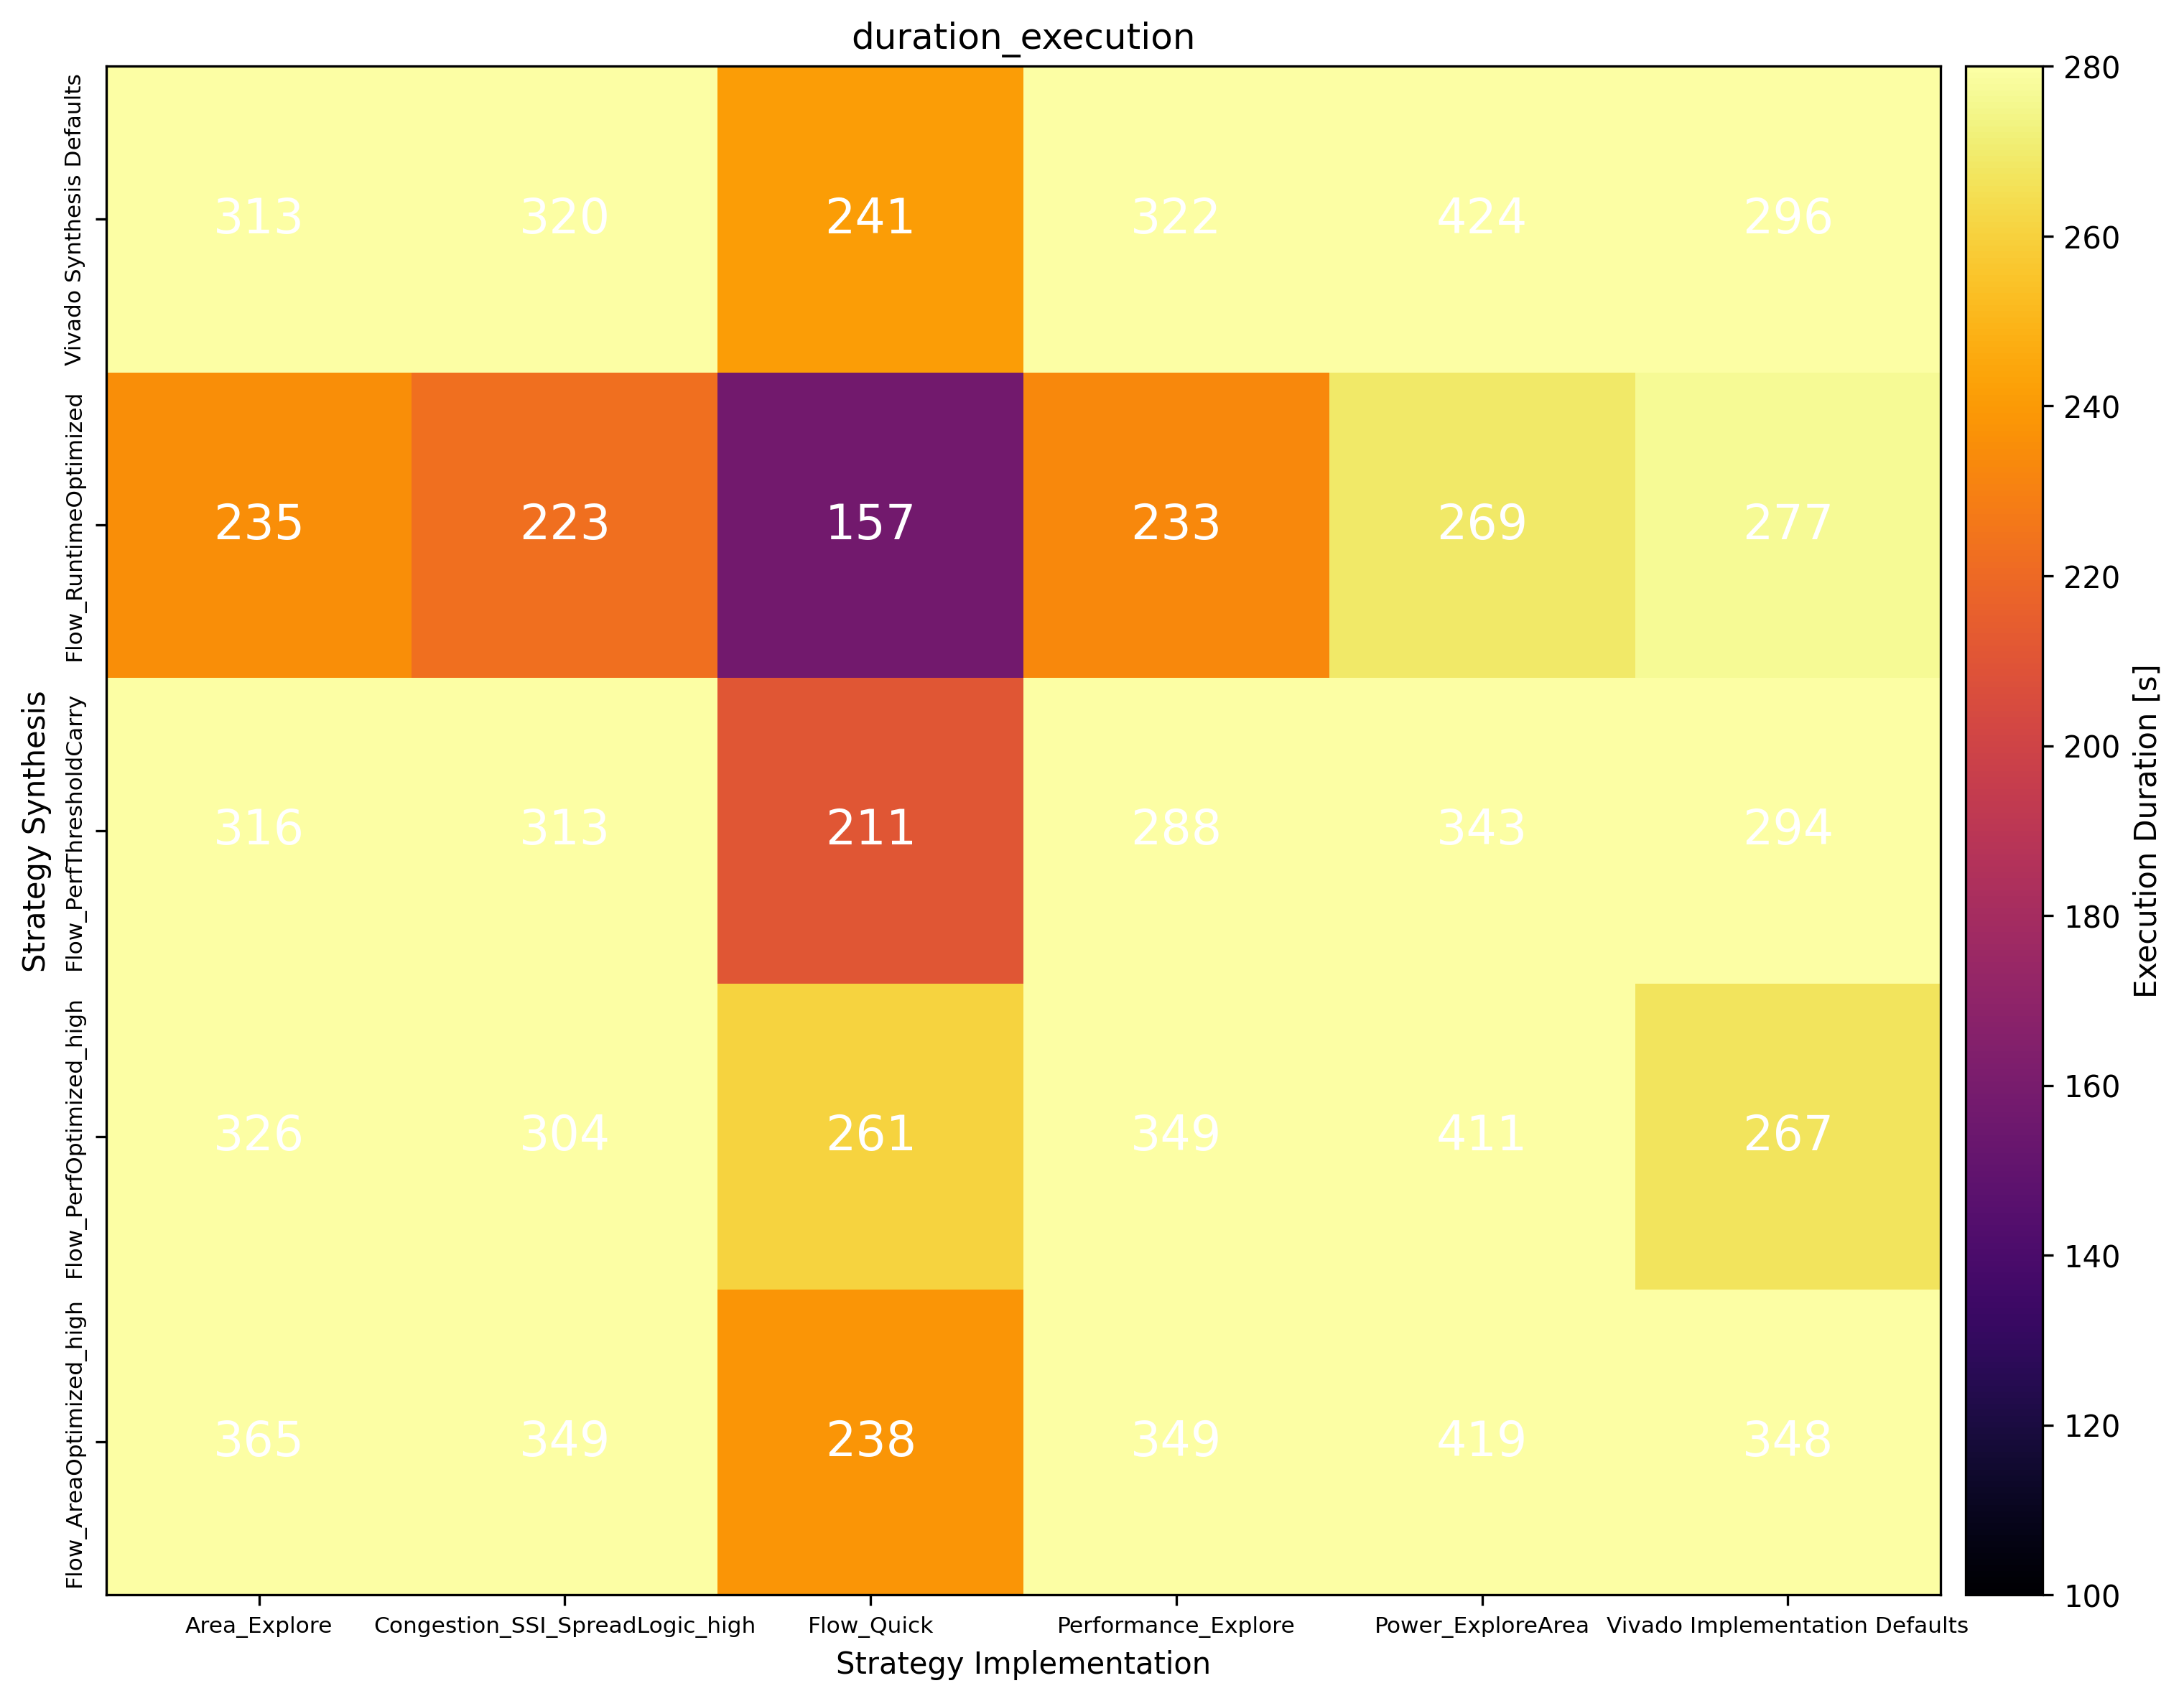
\includegraphics[width=\linewidth]{images/3_duration_execution.png}
        \caption{Duration Totale}
        \label{fig:duration_total_3}
    \end{subfigure}\hfill
	\begin{subfigure}[b]{0.30\textwidth}
        \centering
        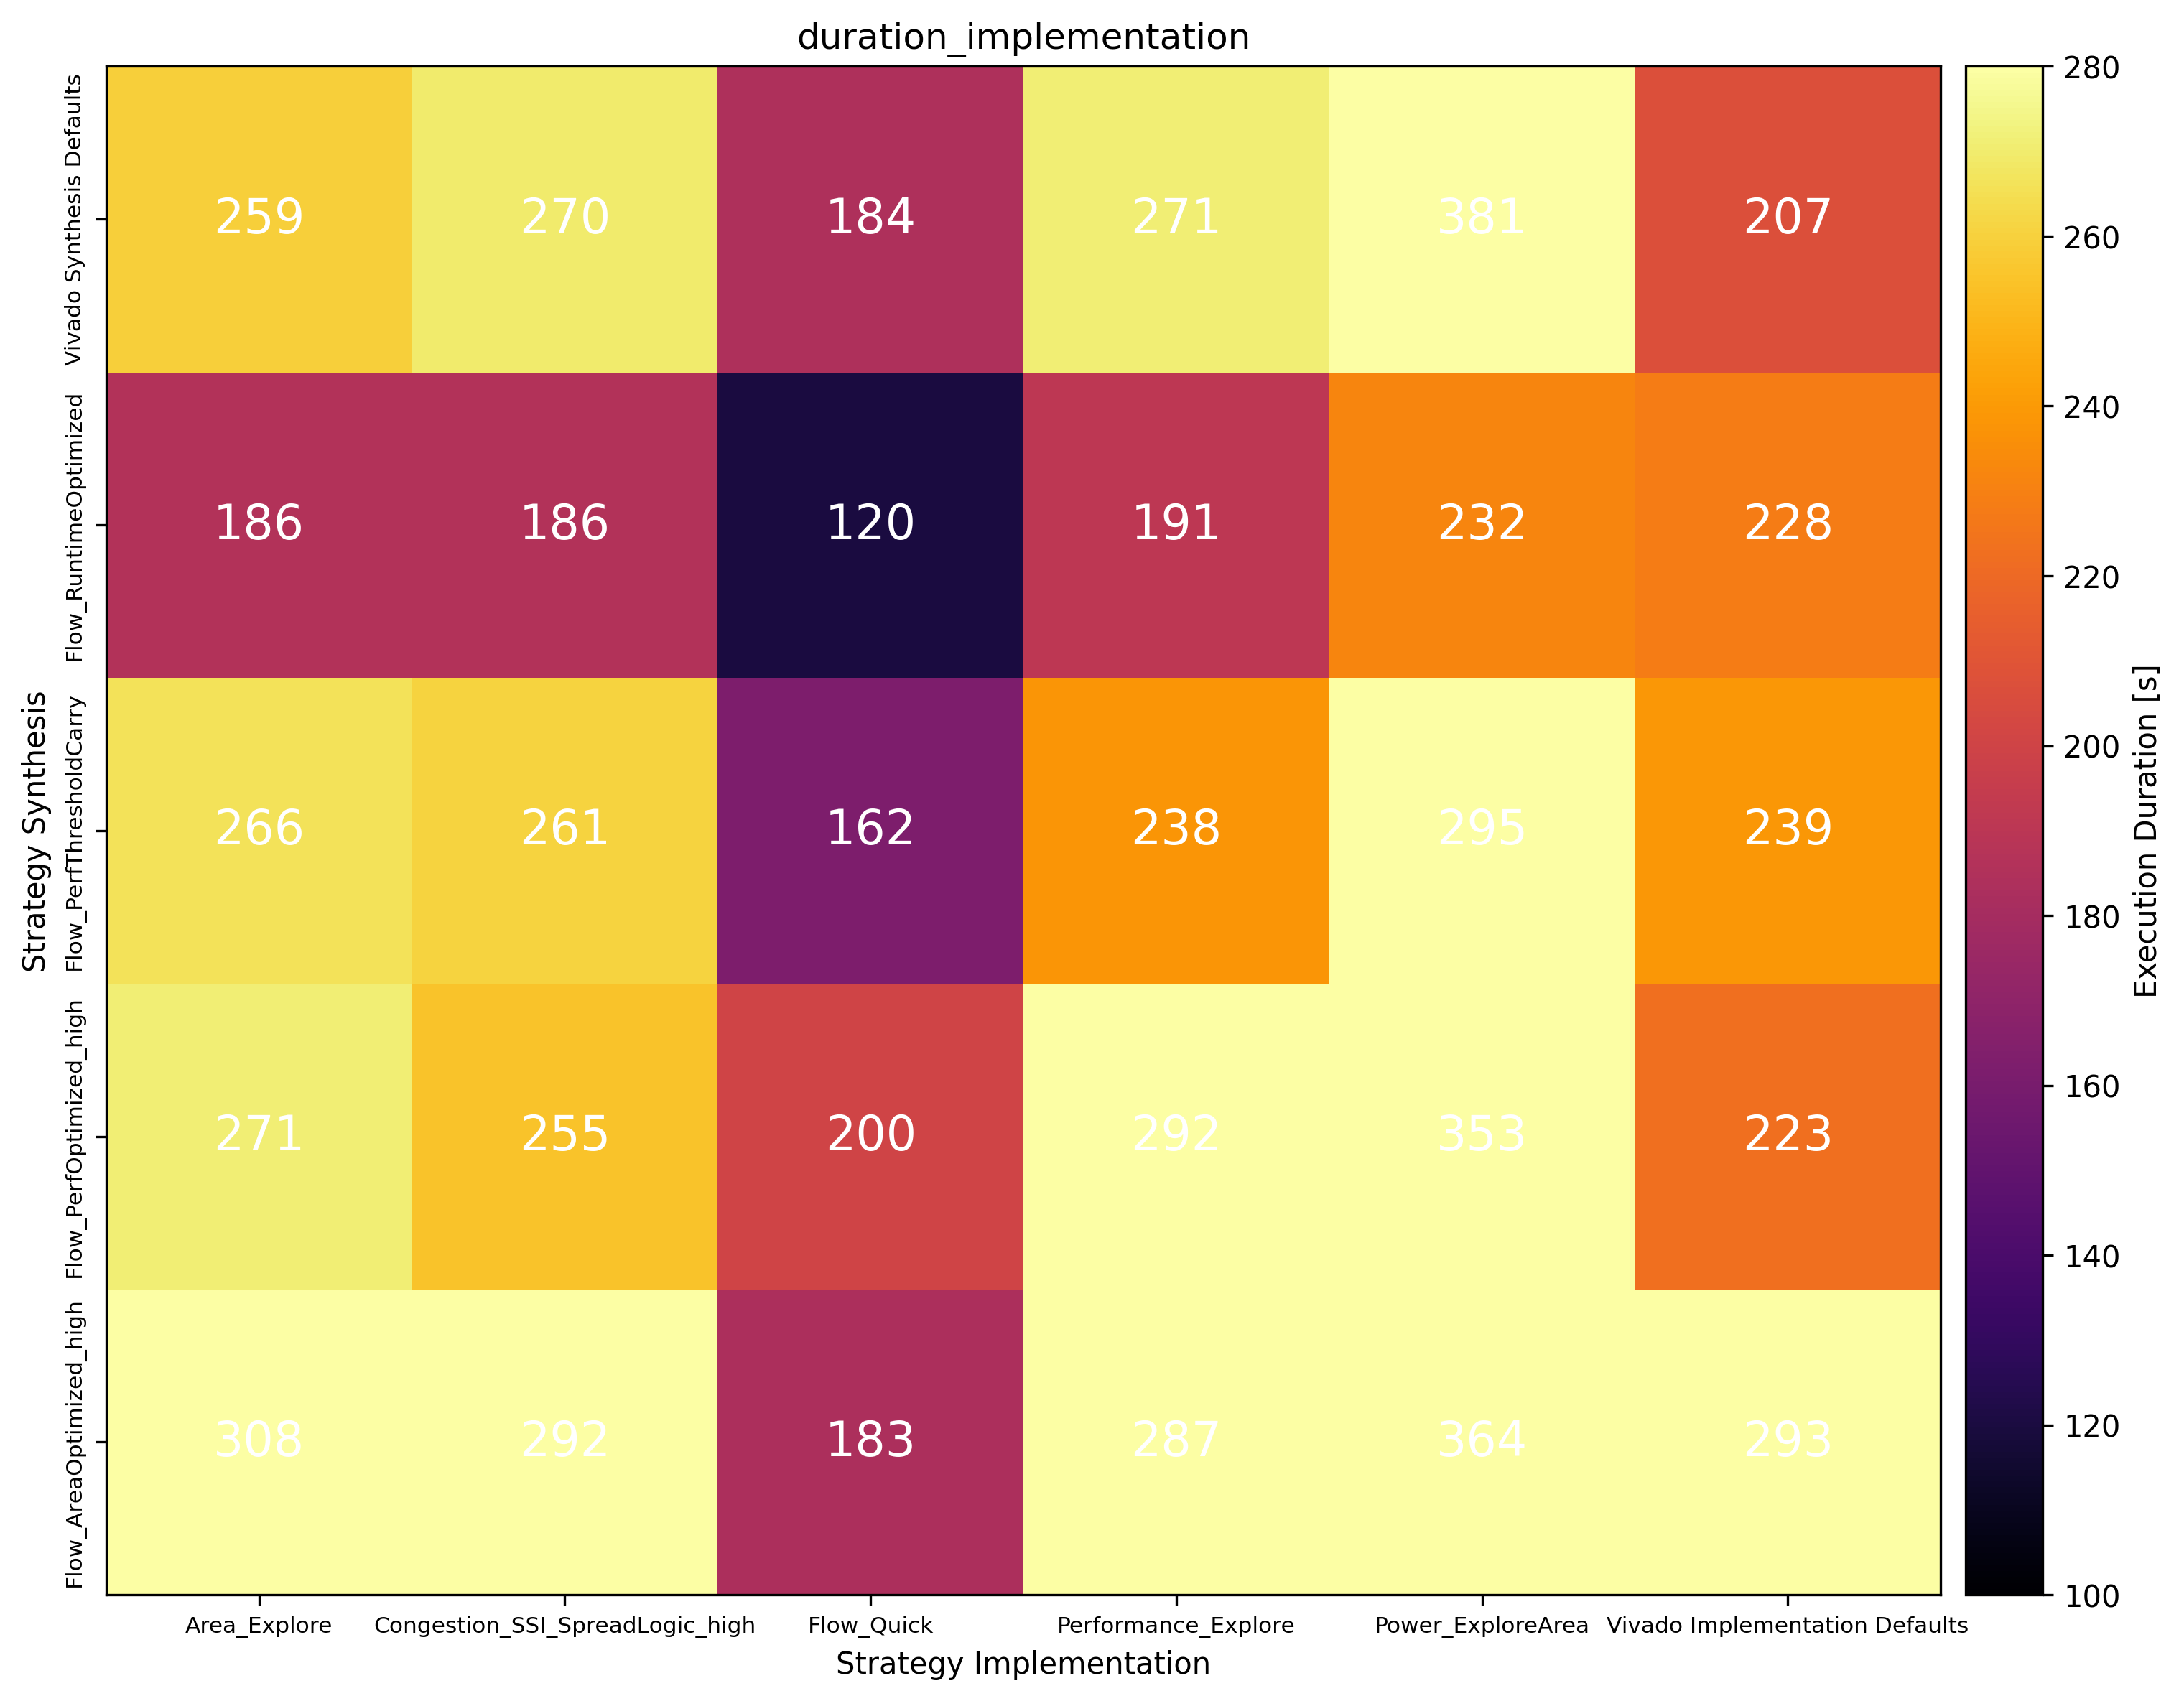
\includegraphics[width=\linewidth]{images/3_duration_implementation.png}
        \caption{Duration Implementation}
        \label{fig:duration_implementation_3}
    \end{subfigure}\hfill
    \begin{subfigure}[b]{0.30\textwidth}
        \centering
        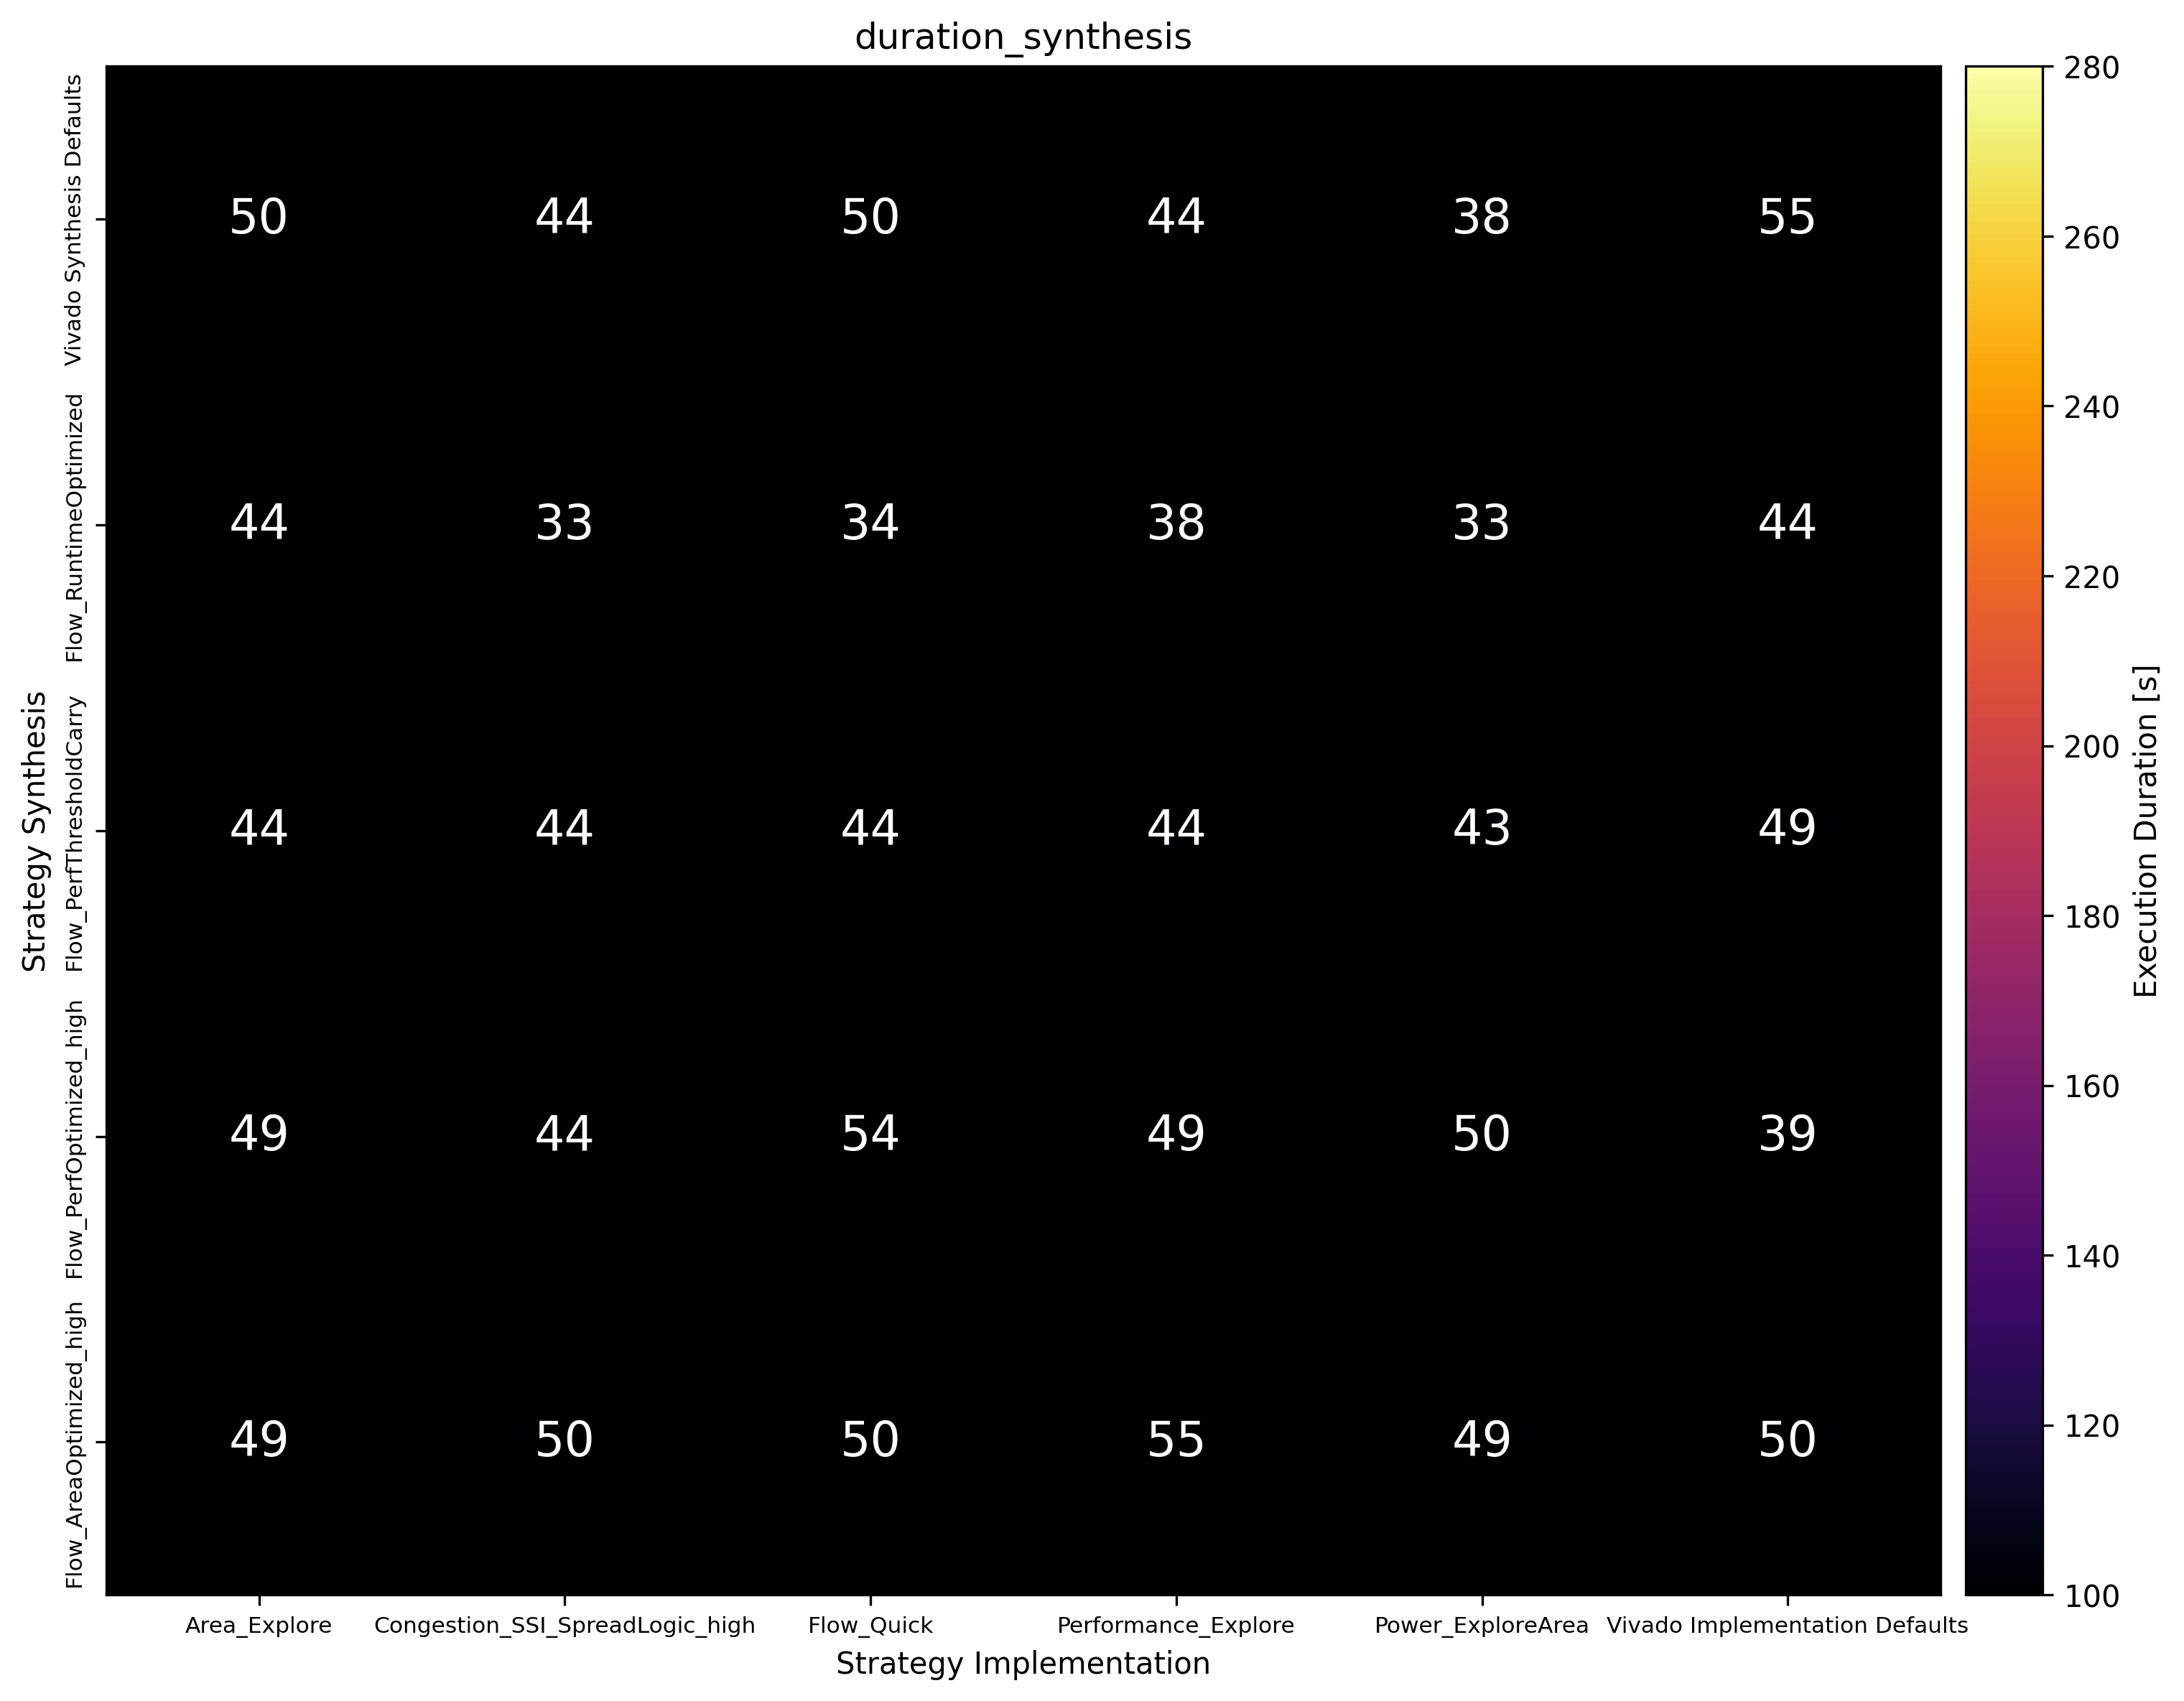
\includegraphics[width=\linewidth]{images/3_duration_synthesis.png}
        \caption{Duration Synthesis}
        \label{fig:duration_synthesis_3}
    \end{subfigure}
    \caption{Temps d'Éxécution de Simulation pour Synthèse et Implémentation}
    \label{fig:duration_3}
\end{figure}
\begin{remark}
    Il faut remarquer que le plus petit le valeur, le mieux.
\end{remark}
\begin{remark}
    Il faut remarquer que la Figure \ref{fig:duration_total_3} est égalé à la somme des Figures \ref{fig:duration_implementation_3} et \ref{fig:duration_synthesis_3}.
\end{remark}
\noindent Il est à noter que, comme expliqué pour la question Q2, la stratégie d'implémentation "Flow\_Quick" présente les temps d'exécution les plus bas, tandis que la stratégie de synthèse "Flow\_RuntimeOptimized" donne des résultats légèrement supérieurs.\\

\noindent On observe également que la stratégie d'implémentation avec les temps d'exécution les plus élevés est "Power\_ExploreArea", avec la méthode "Flow\_RuntimeOptimized" affichant une durée significativement plus longue que toutes les autres. Les autres combinaisons de méthodes ne montrent pas de résultats remarquables.\\

\noindent Comme la même échelle a été utilisée pour les deux cas, il est évident que les temps d'exécution sont généralement plus élevés dans ce cas-ci, ce qui est attendu, étant donné que ce circuit présente une architecture nettement plus sophistiquée.


\subsubsection{Power}
\noindent Ensuite, l'analyse porte sur la puissance dissipée simulée pour les circuits, en fonction de chaque combinaison de synthèse et d'implémentation, comme indiqué ci-dessous :
\begin{figure}[h]
    \centering
    \begin{subfigure}[b]{0.30\textwidth}
        \centering
        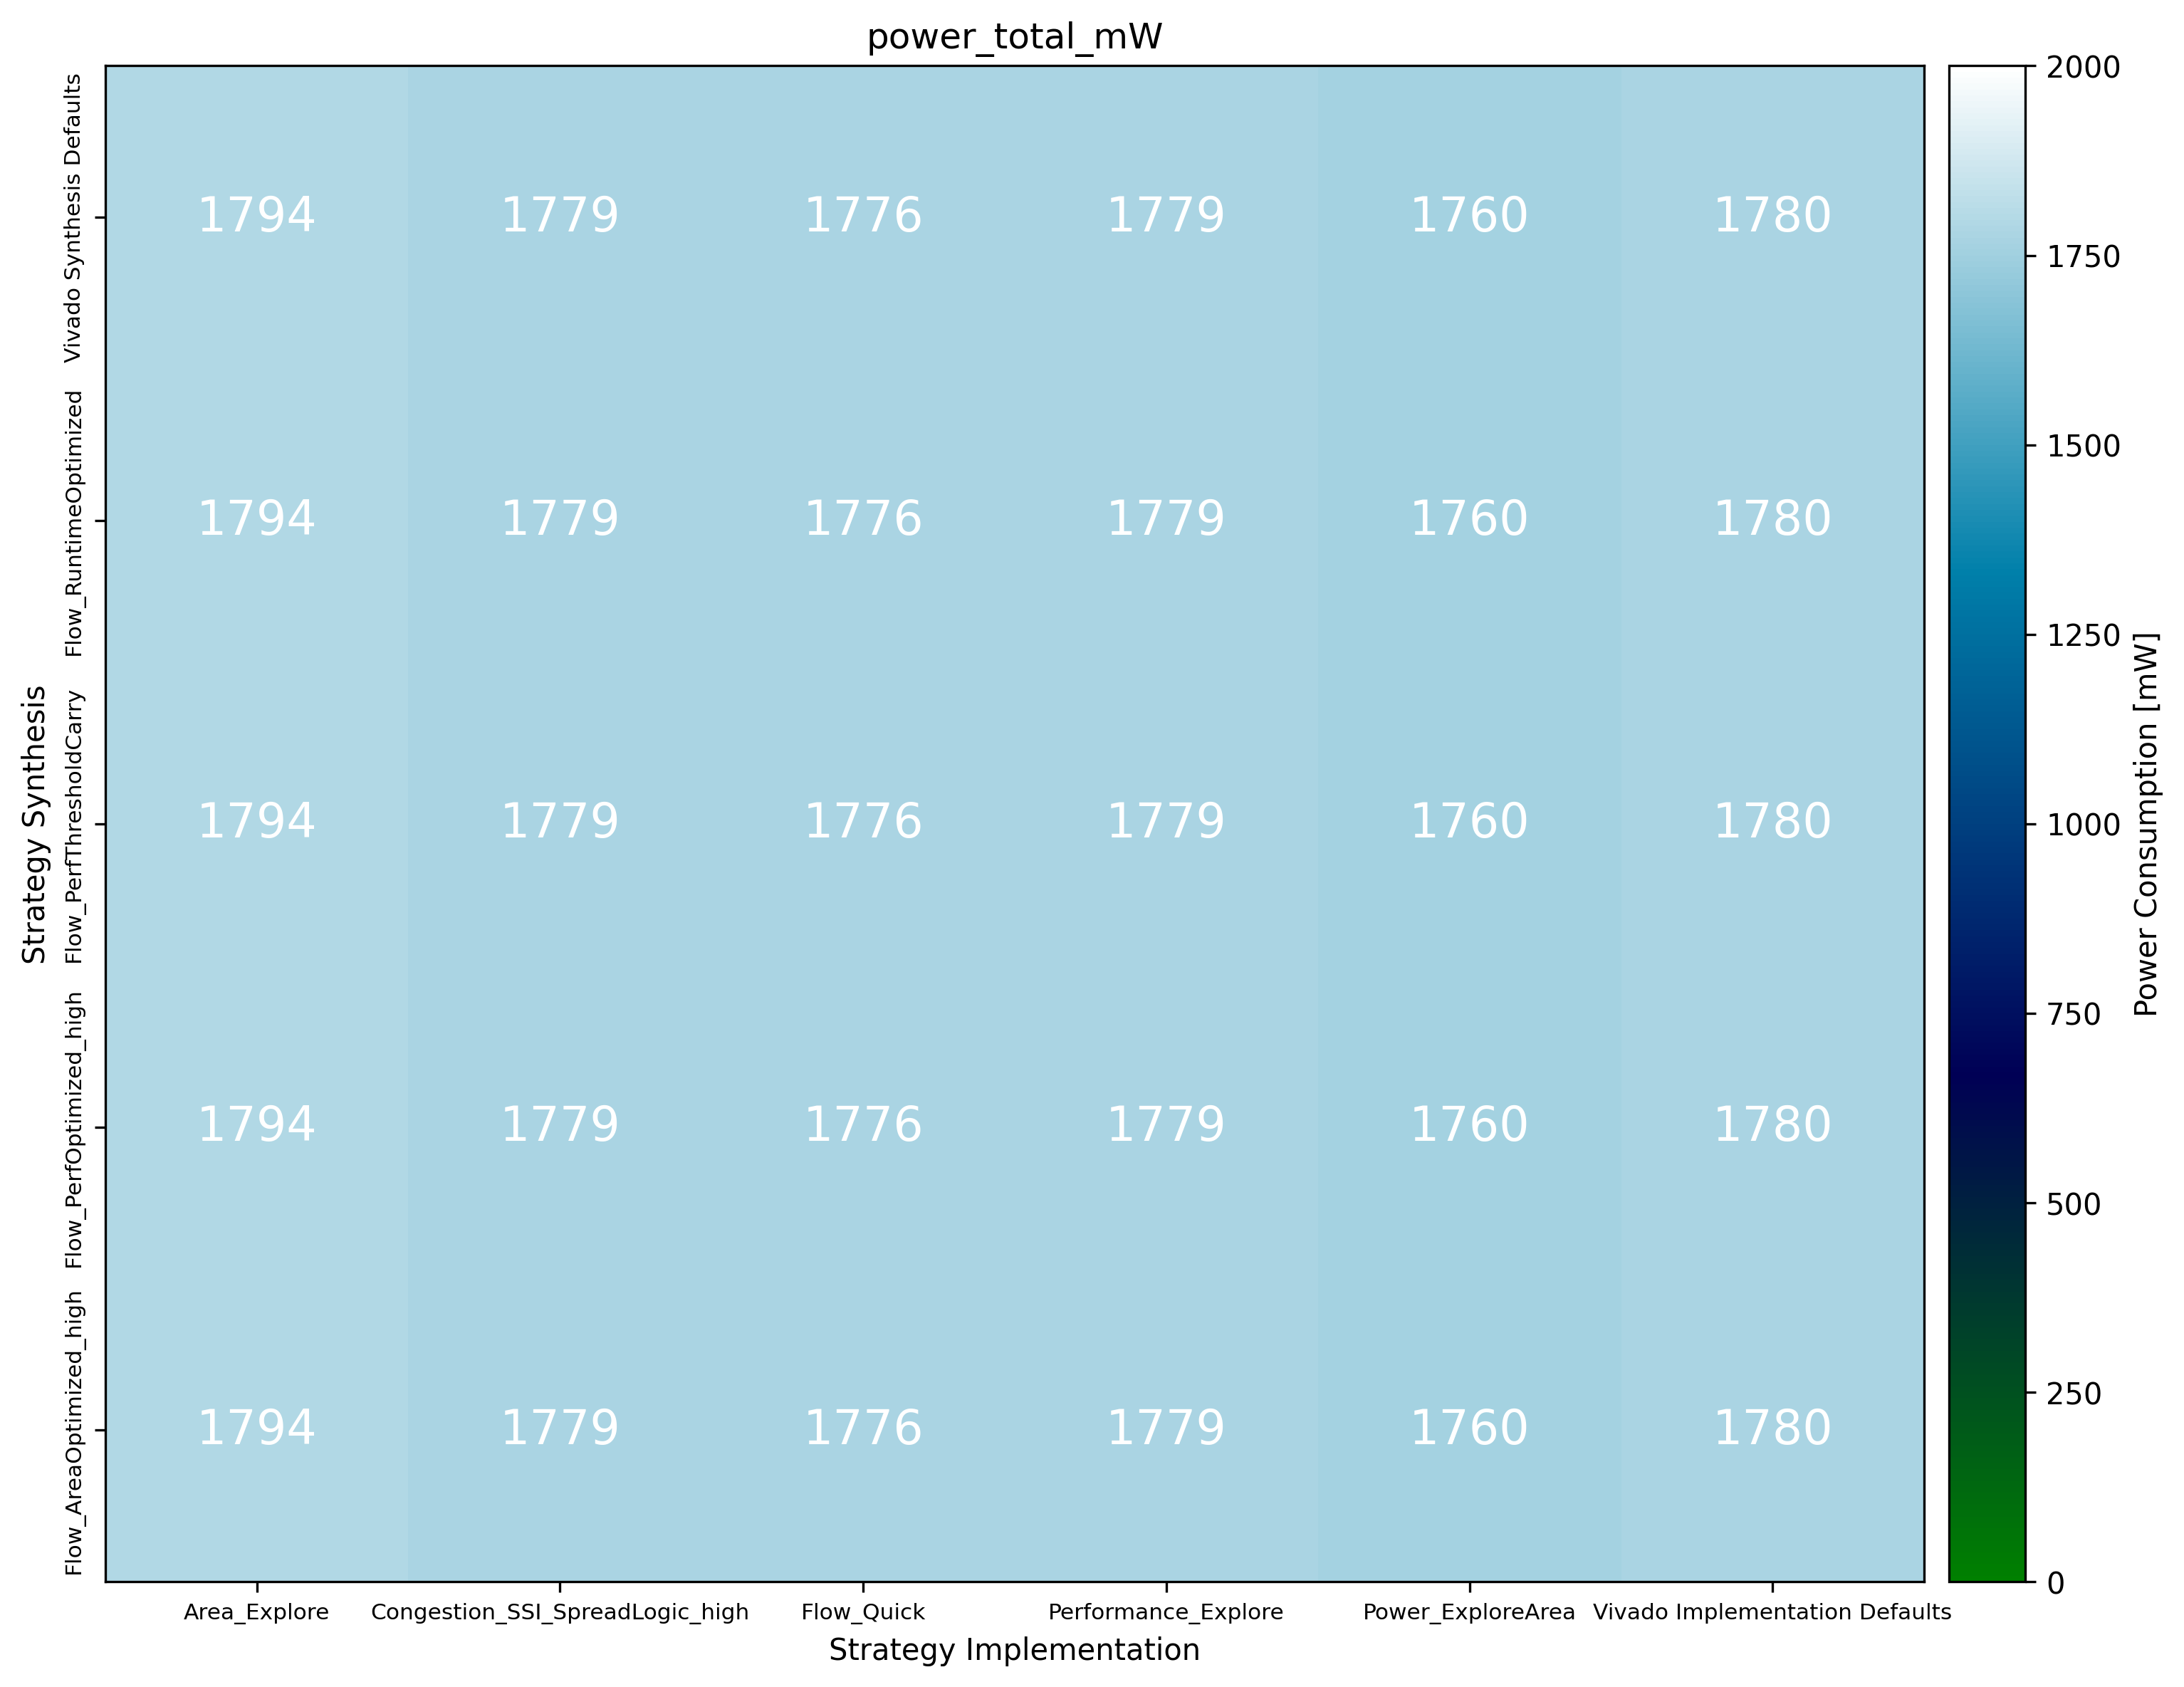
\includegraphics[width=\linewidth]{images/3_power_total_mW.png}
        \caption{Énergie Totale}
        \label{fig:power_total_3}
    \end{subfigure}\hfill
	\begin{subfigure}[b]{0.30\textwidth}
        \centering
        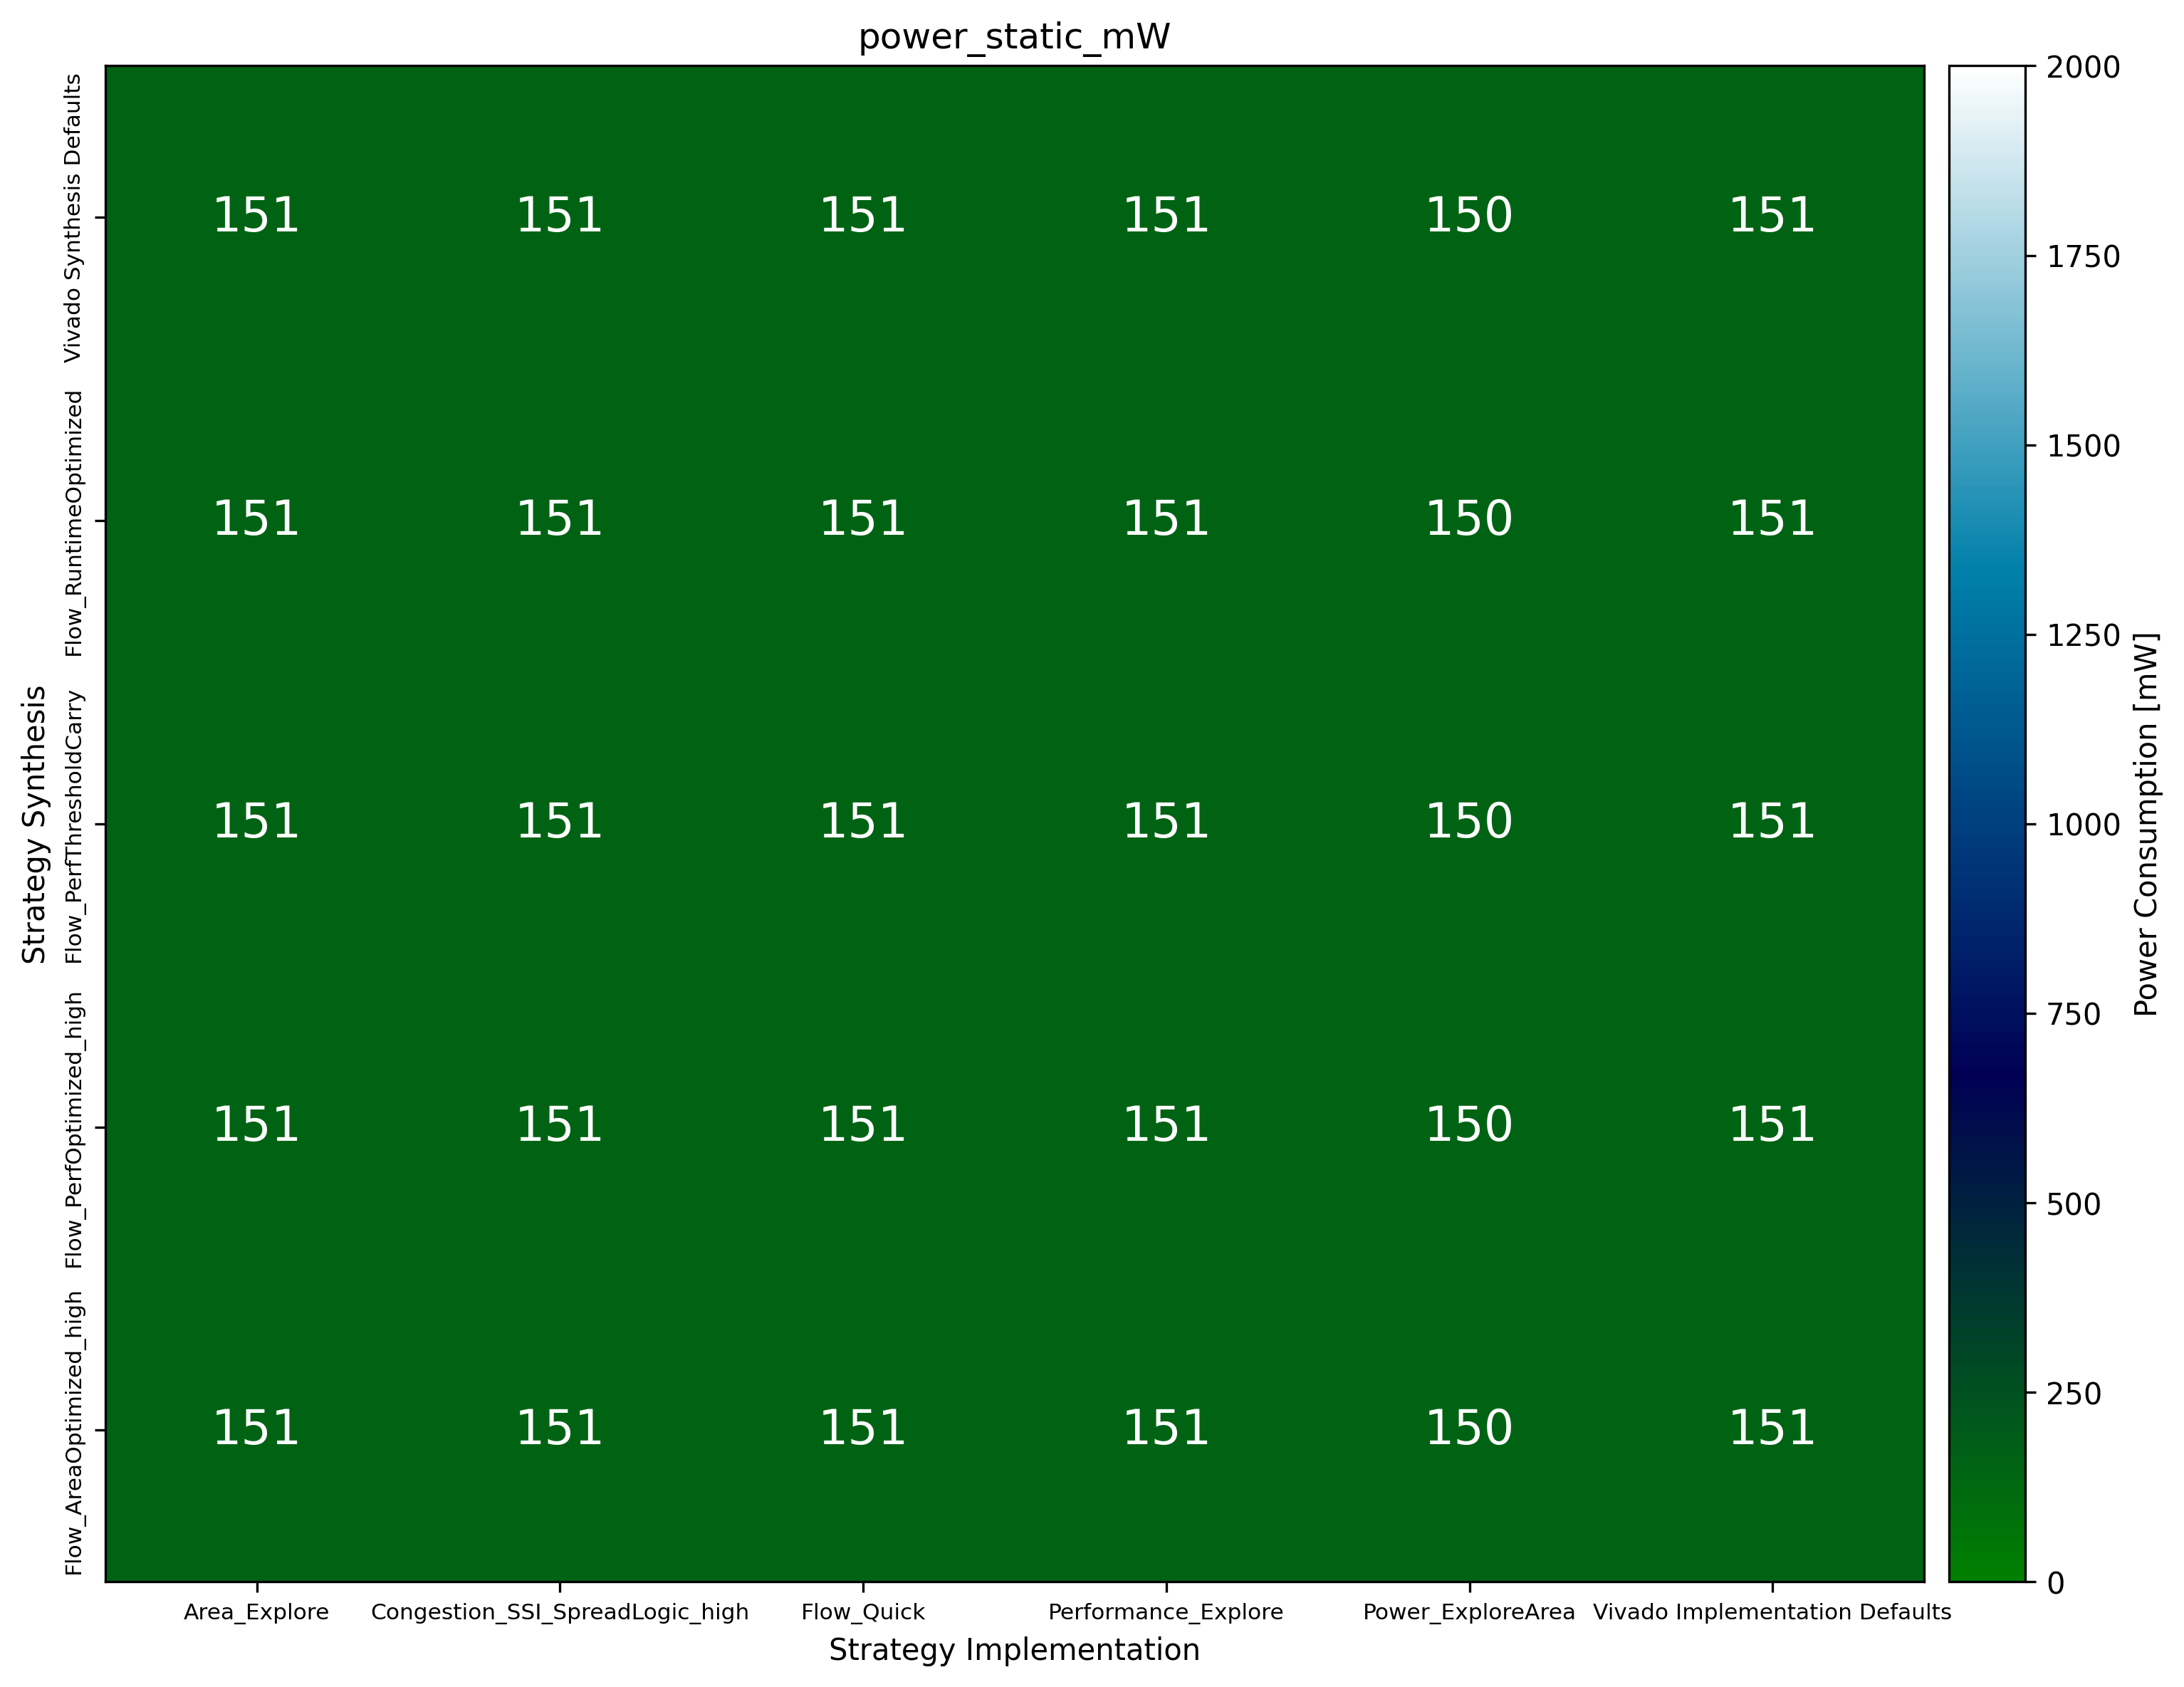
\includegraphics[width=\linewidth]{images/3_power_static_mW.png}
        \caption{Énergie Statique}
        \label{fig:power_static_3}
    \end{subfigure}\hfill
    \begin{subfigure}[b]{0.30\textwidth}
        \centering
        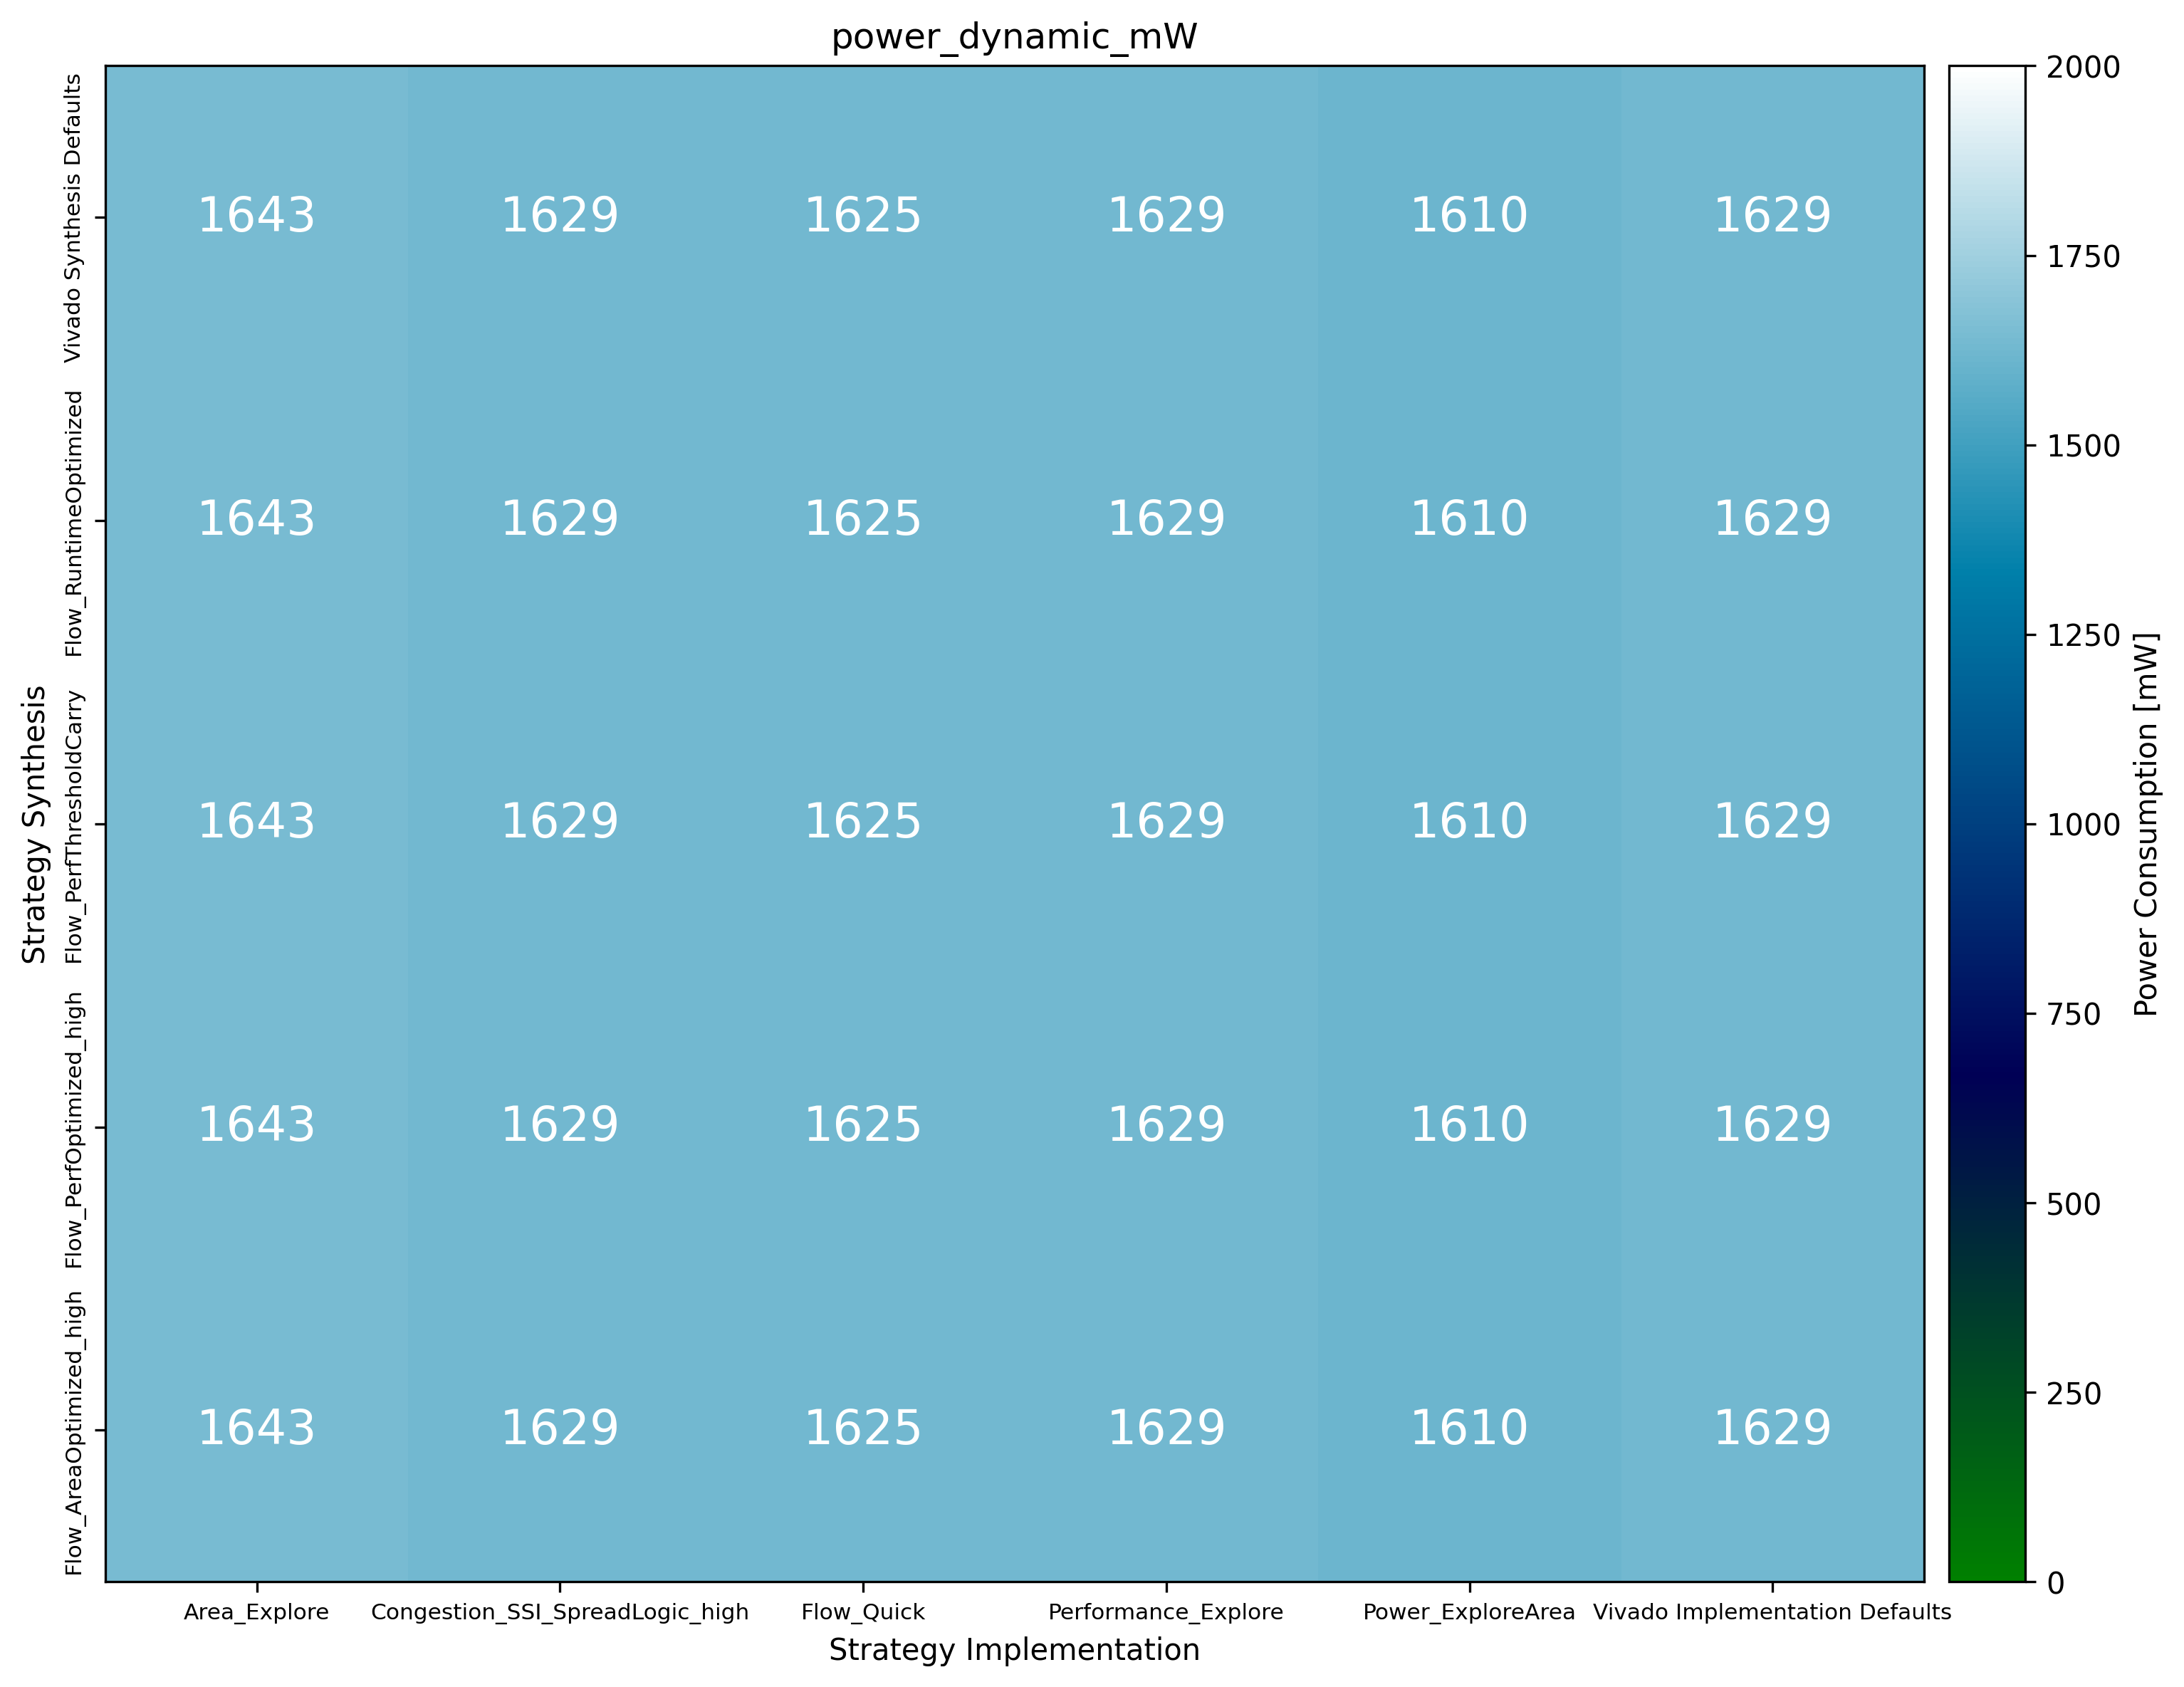
\includegraphics[width=\linewidth]{images/3_power_dynamic_mW.png}
        \caption{Énergie Dynamique}
        \label{fig:power_dynamic_3}
    \end{subfigure}
    \caption{Dissipacition d'Énergie de Simulation pour Synthèse et Implémentation}
    \label{fig:power_3}
\end{figure}
\begin{remark}
    Il faut remarquer que le plus petit le valeur, le mieux.
\end{remark}
\begin{remark}
    Il faut remarquer que la Figure \ref{fig:power_total_3} est égalé à la somme des Figures \ref{fig:power_static_3} et \ref{fig:power_dynamic_3}.
\end{remark}
\noindent Il est à noter que, comme pour la question Q2, les valeurs sont pratiquement identiques et qu'il n'y a pas de grande variabilité entre les différentes valeurs.\\

\noindent Ainsi, une analyse plus détaillée a été effectuée sur les configurations qui ont donné les meilleurs et les pires résultats en termes de temps d'exécution :
\begin{figure}[H]
    \centering
    \begin{subfigure}[b]{0.475\textwidth}
        \centering
        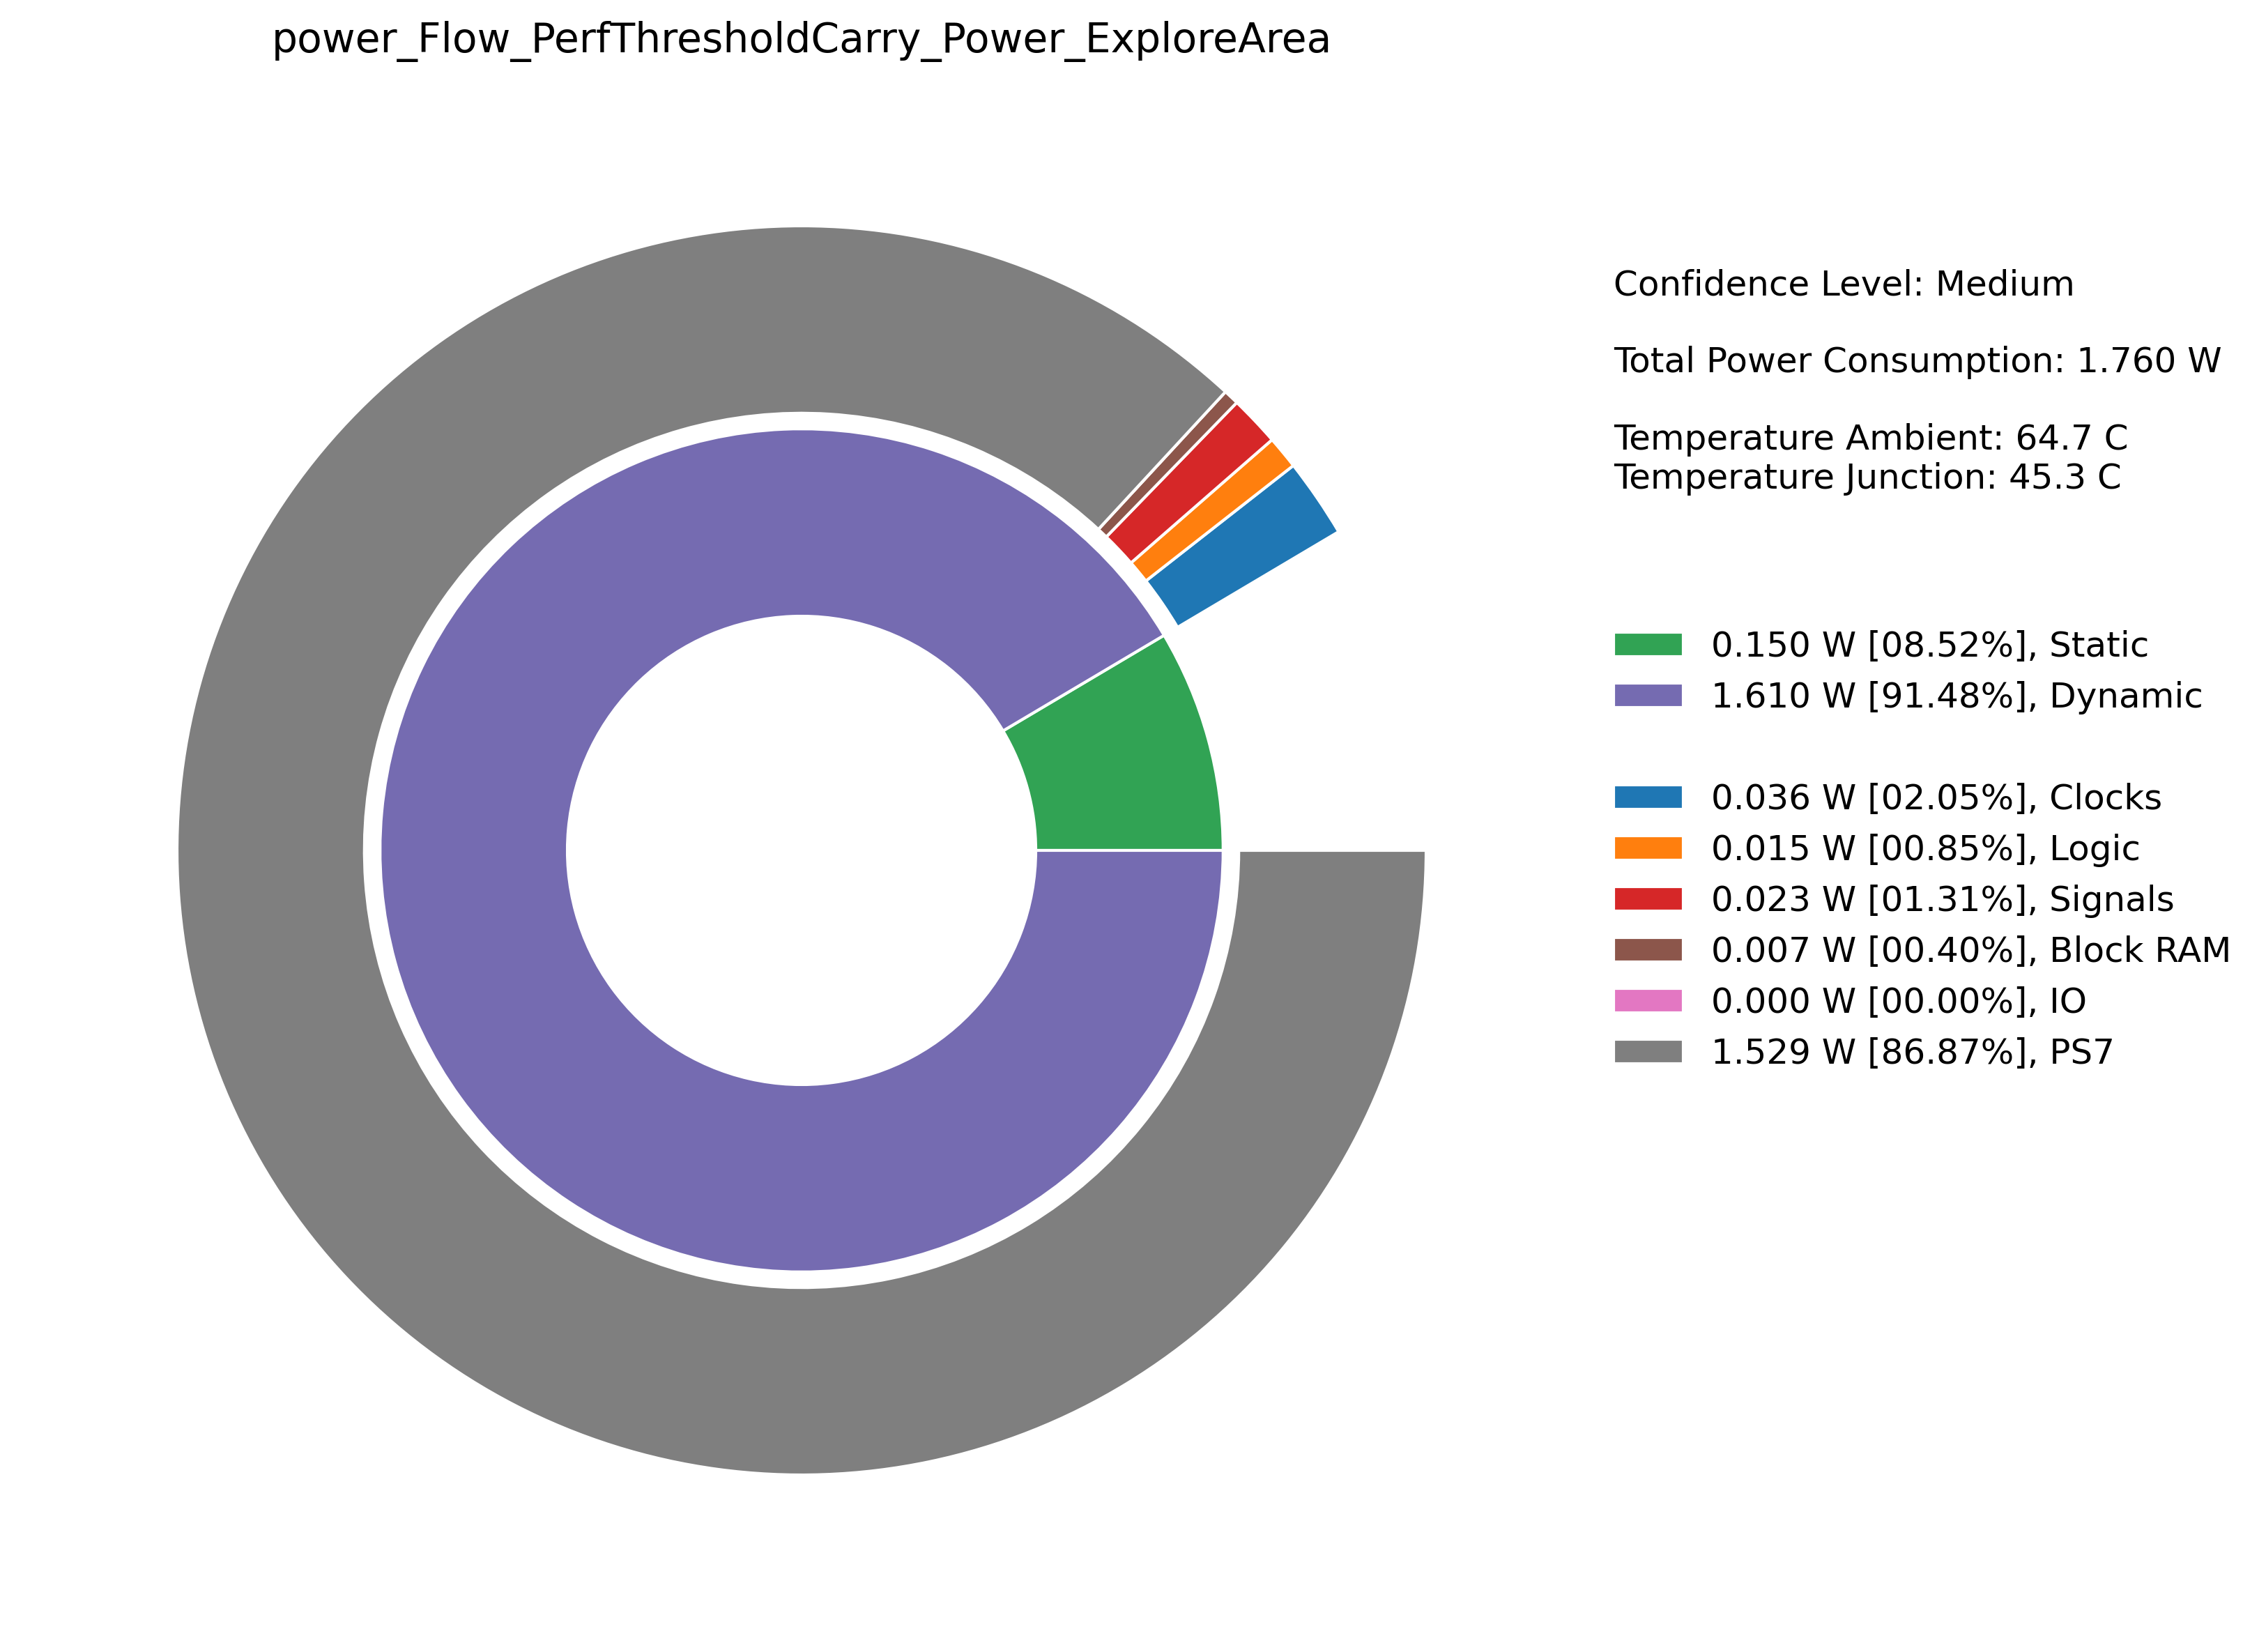
\includegraphics[width=\linewidth]{images/3_power_Flow_PerfThresholdCarry_Power_ExploreArea.png}
        \caption{\texttt{Flow\_PerfThresholdCarry} et \texttt{Power\_ExploreArea}}
    \end{subfigure}\hfill
    \begin{subfigure}[b]{0.475\textwidth}
        \centering
        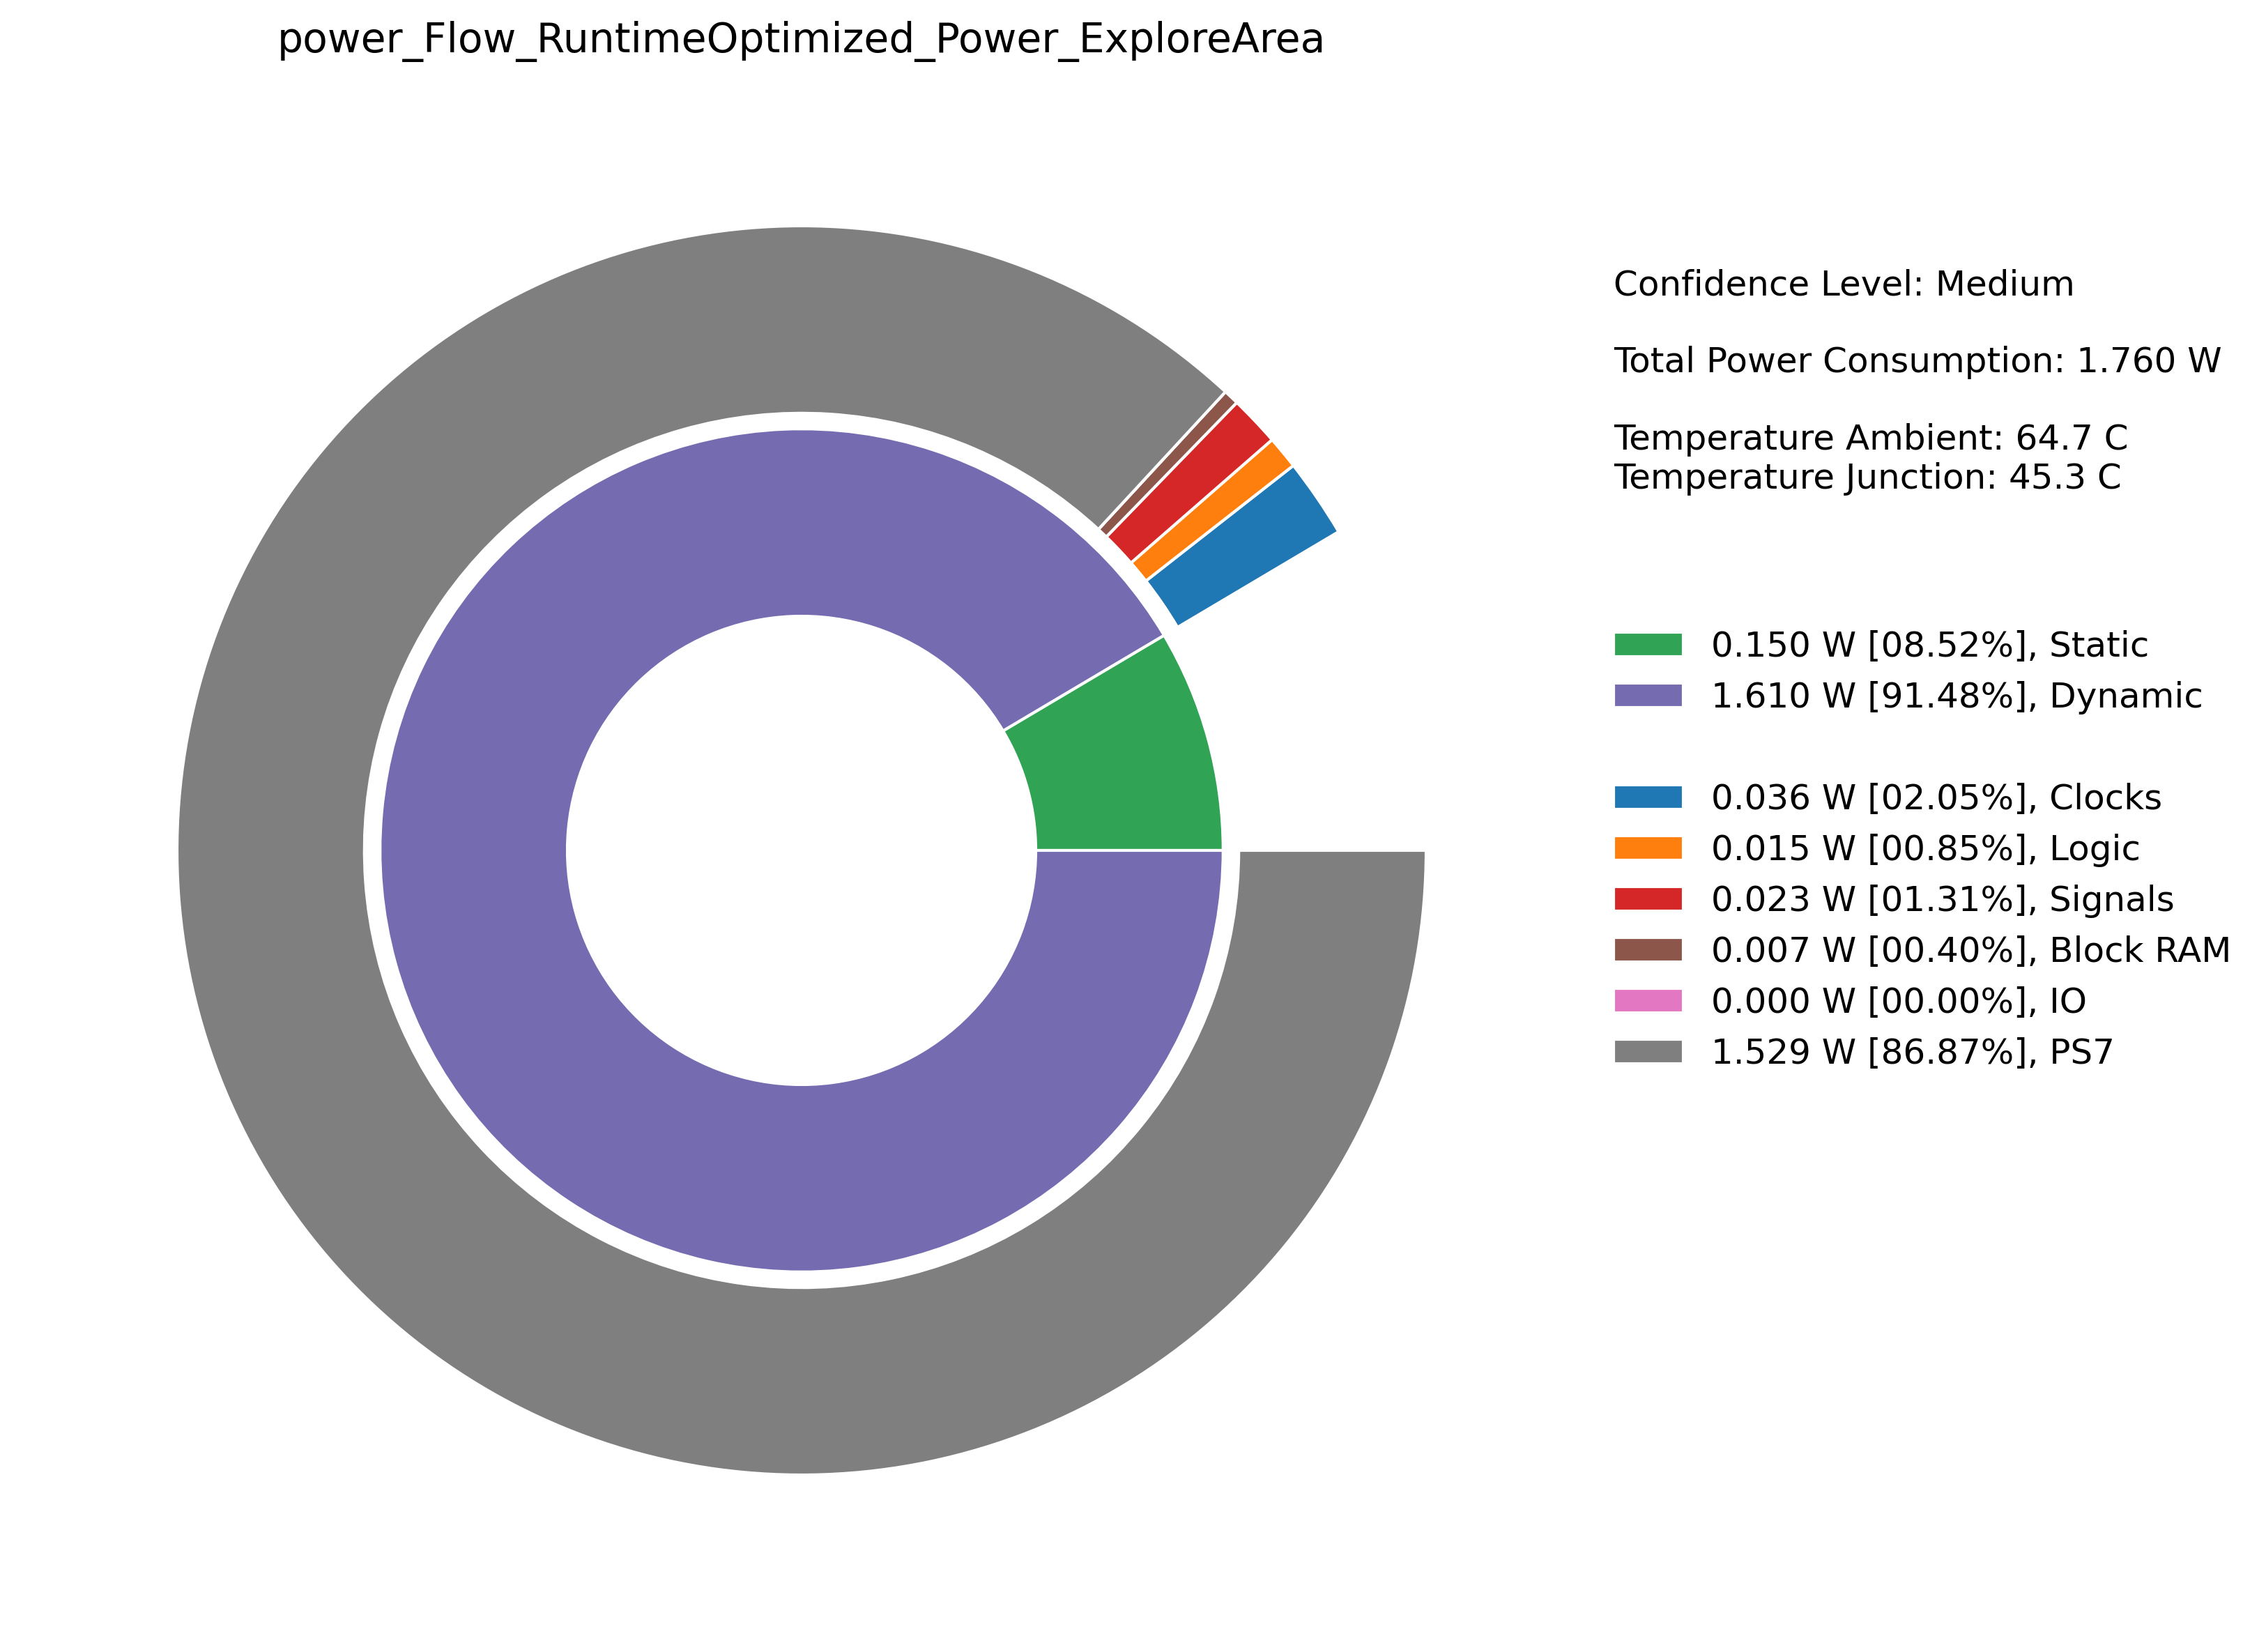
\includegraphics[width=\linewidth]{images/3_power_Flow_RuntimeOptimized_Power_ExploreArea.png}
        \caption{\texttt{Flow\_RuntimeOptimized} et \texttt{Power\_ExploreArea}}
    \end{subfigure}
    \caption{Détail de Dissicipation d'Énergie}
    \label{fig:power_detail_3}
\end{figure}
\noindent Il n'y a pas de grande variabilité entre les différentes combinaisons, et ainsi, il est conclu que la puissance dissipée est peu influencée par les méthodes d'implémentation ou de synthèse utilisées.


\subsubsection{WNS}
\noindent Nous passons maintenant à l'analyse du Worst Negative Slack (WNS) pour les différentes combinaisons de synthèse et d'implémentation, comme démontré ci-dessous :
\begin{figure}[H]
	\centering
	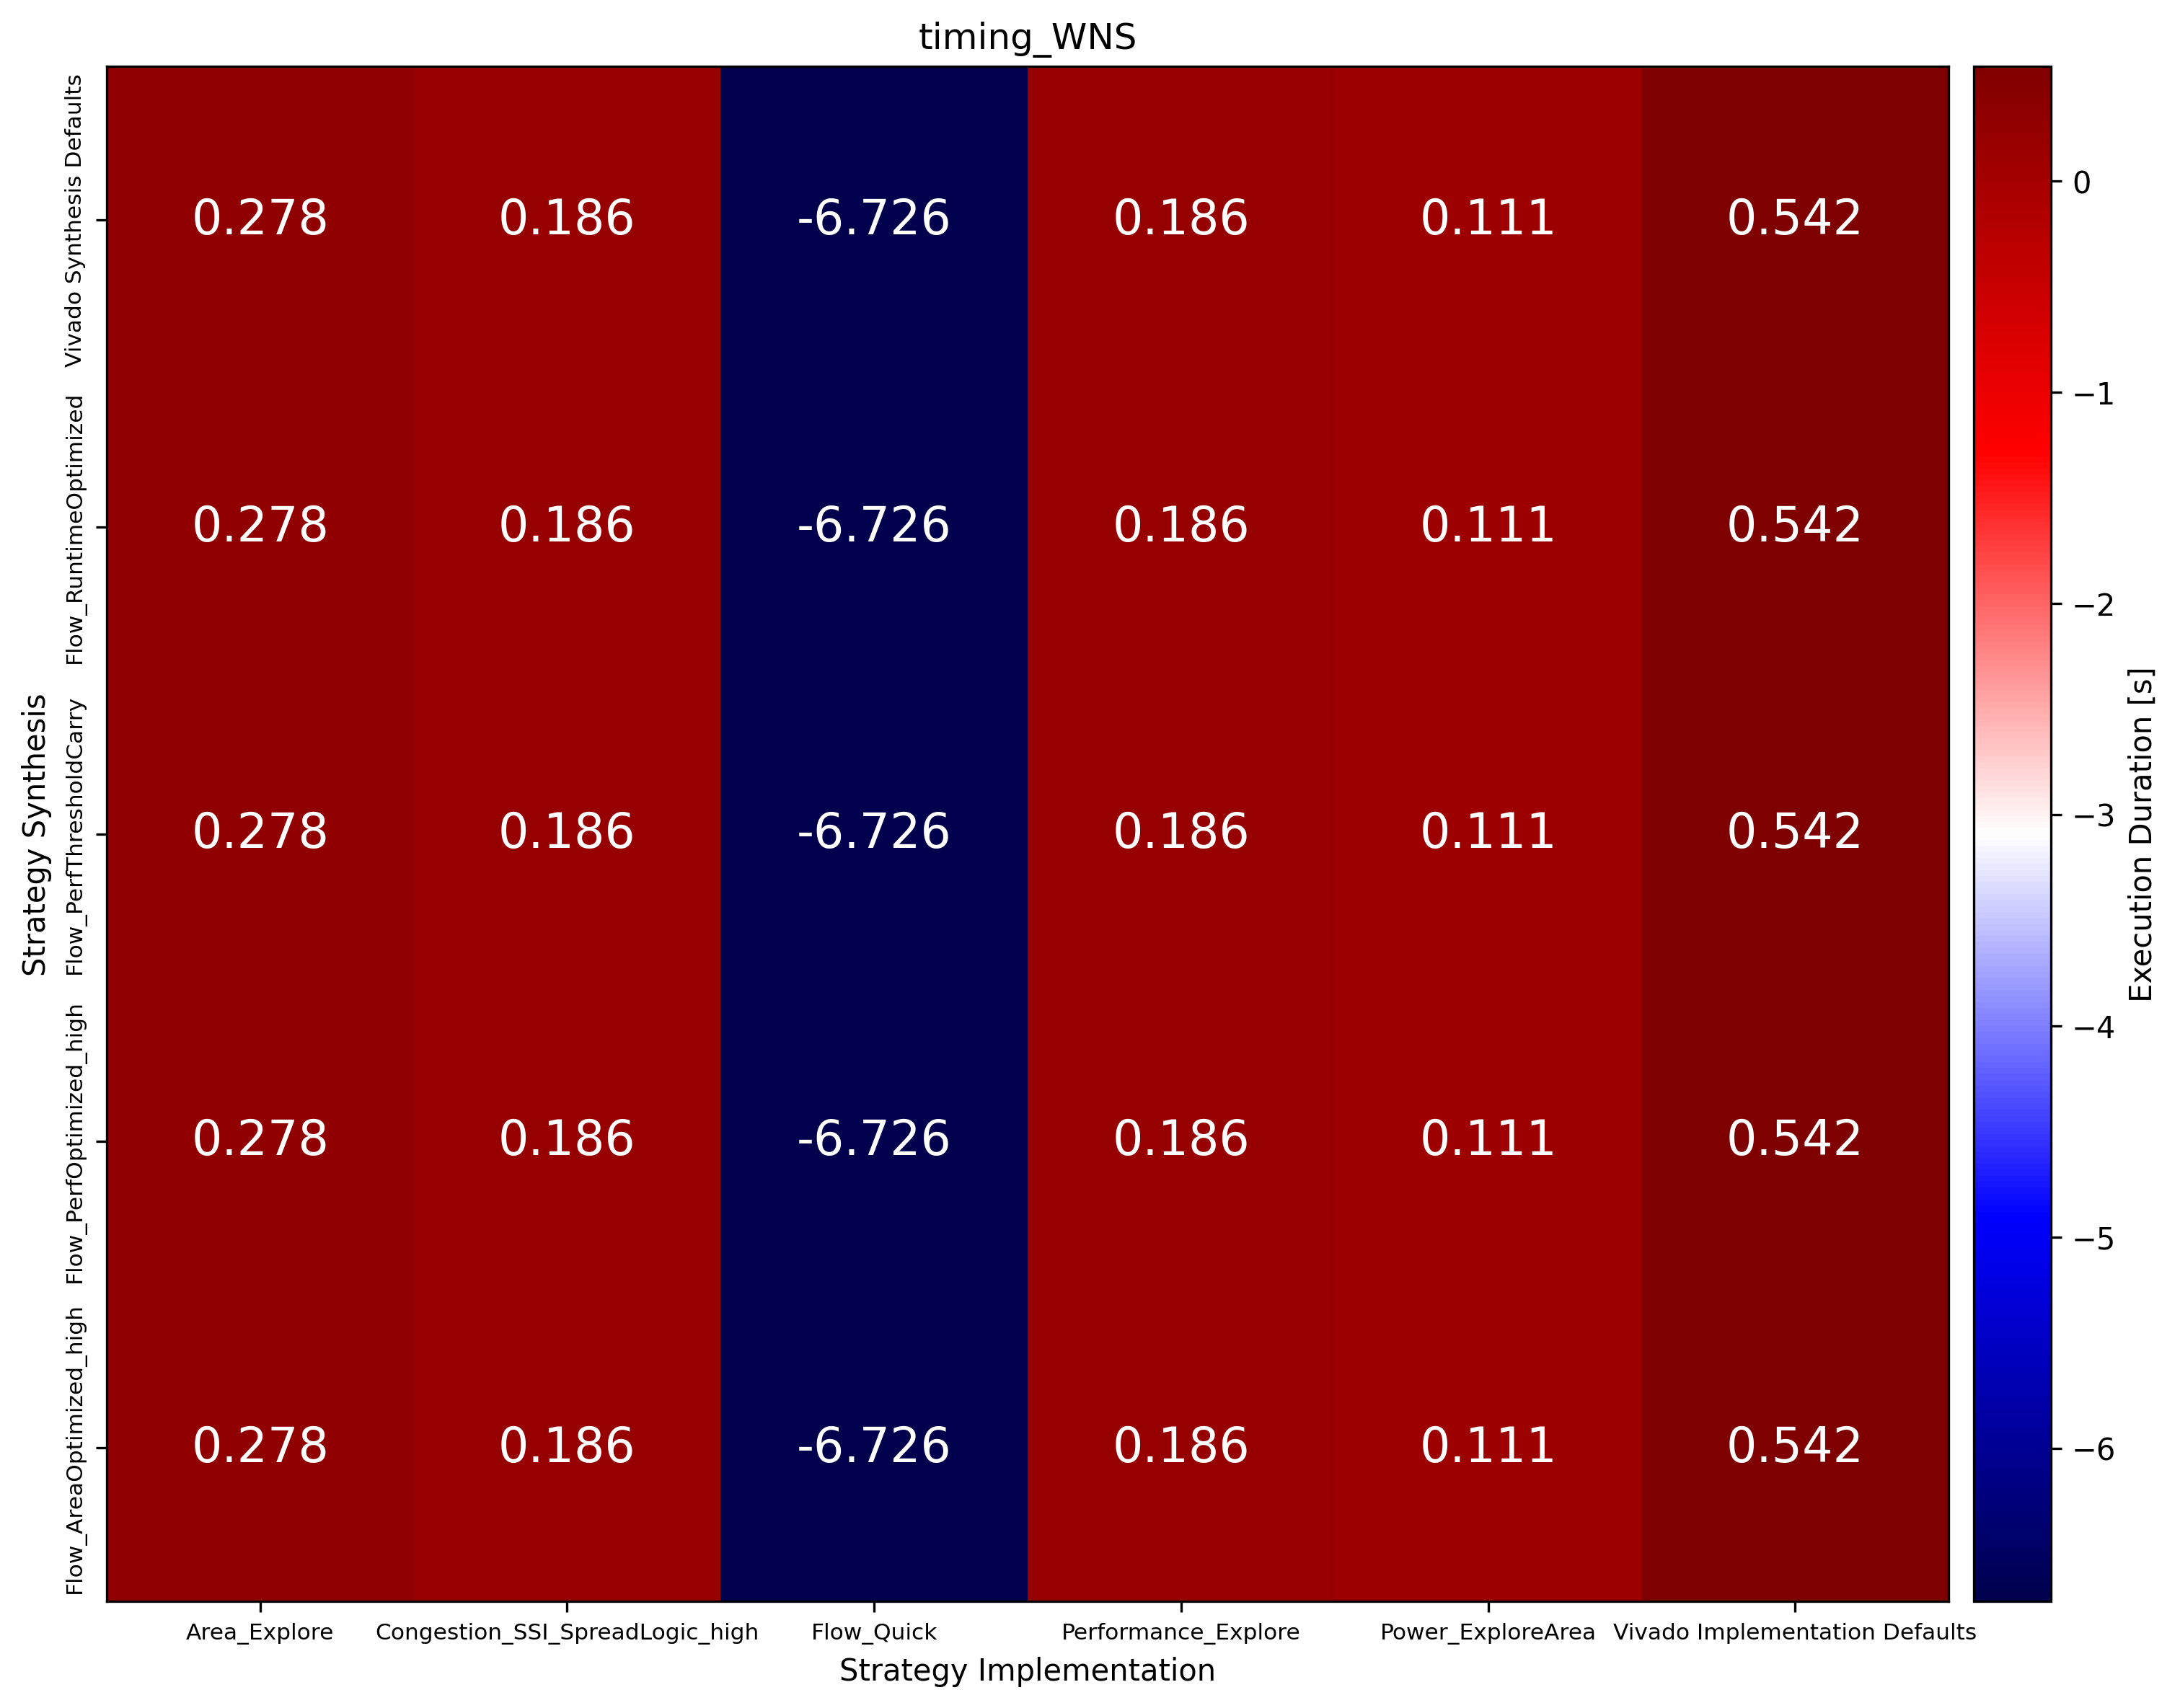
\includegraphics[width=0.5\linewidth]{images/3_timing_WNS.png}
	\caption{WNS Timing pour Synthèse et Implémentation}
	\label{fig:wns_3}
\end{figure}
\begin{remark}
    Il faut remarquer que le plus proche de zéro, le mieux. En cas négatif, sous-optimale.
\end{remark}
\noindent Comme observé pour Q2, le pire résultat est obtenu avec la stratégie d'implémentation "Flow\_Quick" et le meilleur avec "Power\_ExploreArea". La différence entre les résultats est plus significative dans ce cas que dans le précédent, ce qui indique que la complexité de l'architecture implémentée a un impact important sur les gains, ou non, des méthodes d'optimisation.


\subsubsection{Ressources}
\noindent Enfin, l'analyse de l'utilisation des ressources pour les différentes combinaisons de synthèse et d'implémentation est présentée ci-dessous :
\begin{figure}[H]
	\centering
	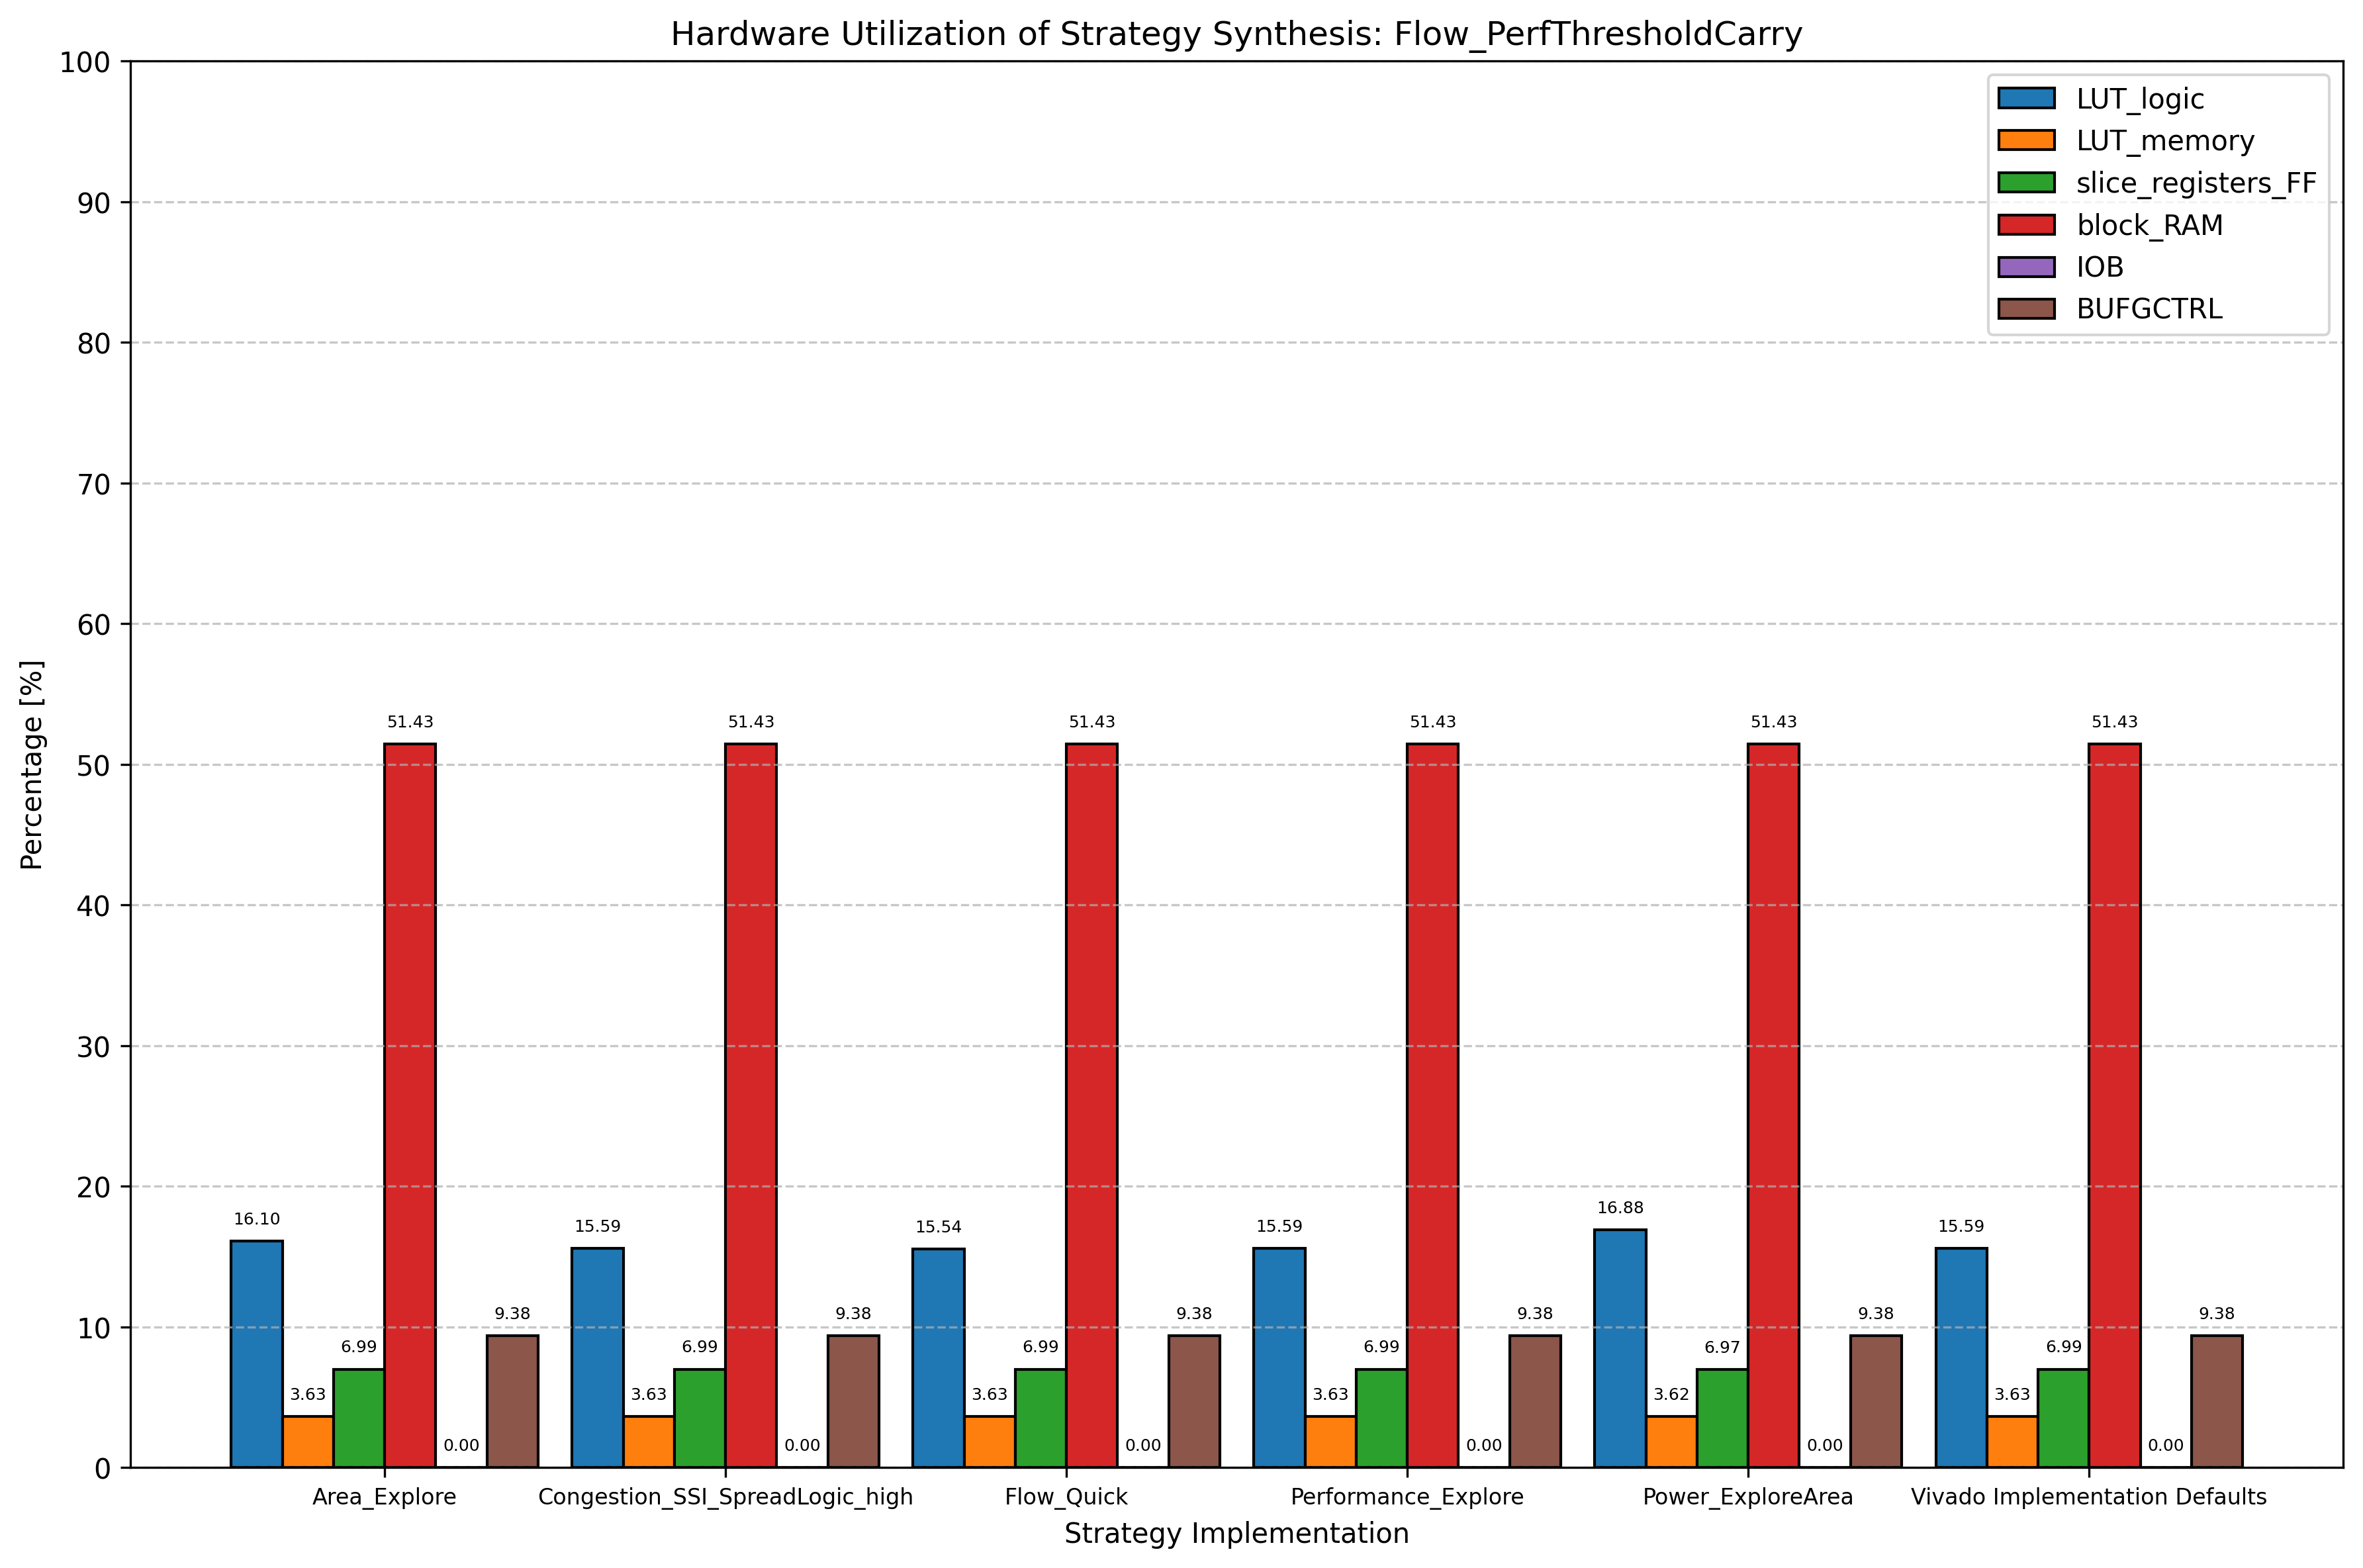
\includegraphics[width=0.5\linewidth]{images/3_utilization_Flow_PerfThresholdCarry.png}
	\caption{Utilization de Ressources pour \texttt{Flow\_PerfThresholdCarry}}
	\label{fig:ressouces_3}
\end{figure}
\begin{remark}
    Il faut remarquer que le plus petit, le mieux.
\end{remark}
\noindent Encore une fois, on remarque qu'il n'y a pas de grande variabilité entre les différentes options d'implémentation. Cependant, toutes les parties du matériel sont plus sollicitées dans ce cas que dans le cas précédent.

\subsection{Résultats Généraux}
\noindent En résumé, on peut observer que les résultats obtenus expérimentalement subissent de petites modifications lorsque l'on manipule des stratégies et des algorithmes d'optimisation. Bien que de petits gains puissent être obtenus en utilisant les outils disponibles dans Vivado, la capacité à concevoir une architecture efficace et optimisée influence beaucoup plus fortement le résultat final.\\

\noindent Ainsi, il est important de souligner l'importance de travailler avec soin lors de la conception des différentes parties du matériel et du logiciel afin d'obtenir les meilleurs résultats possibles avec le matériel disponible, car l'optimisation du logiciel et du matériel ne peut compenser une architecture mal conçue.
\end{document}
